\documentclass{llncs}

\usepackage{graphicx}
\usepackage{makeidx}
\usepackage{todonotes}
\usepackage{amsmath}
\usepackage{algorithmic}
\usepackage[margin=1in]{geometry}

\begin{document}

\mainmatter
\title{Modeling Heterogeneous Traffic Performance \\ with the 802.11 DCF Access Scheme}
\author{Tamir Husain and Christopher A. Wood}
\maketitle

\begin{abstract}
We study the random behavior of the 802.11 DCF protocol for wireless LANs that serve heterogeneous traffic. Our study is based on a novel paramterized Markov model, which can be tuned according to the packet interarrival time, packet buffer arrival probability, packet length, and interarrival wait probability associated with any type of application traffic. Using these parameterized model templates, we instantiate individual instances with parameters drawn from realistic statistical characterizations of modern application traffic, such as web browsing, file downloads, and multimedia traffic. Assuming a fixed network-wide conditional collision probability, we then emulate the behavior of the DCF access scheme within the context of a single node. Following this, we combine these individual model instances to study the performance of the DCF function with respect to heterogeneous traffic in a true multi-node system. Our experimental results provide evidence that the deterministic nature of multimedia (e.g., store-and-forward) traffic streams leads to higher performance (i.e., higher throughput) than more nondeteministic (elastic) traffic. Furthermore, our results show that large interarrival time between traffic packets benefits the coexistence of heterogeneous traffic streams. 
\end{abstract}

\section{Introduction}
Wireless networks have become pervasive in modern computer and communication systems. The widespread adoption of mobile and personal computing devices, such as smartphones and tablets, continues to drive commercial investment in high performance wireless networking technologies. Concurrently, the type of traffic traversing these networks has also evolved -- divergently -- an increasing rate. Every kind of information from textual data to video stream segments now traverses wireless networks. Society's dependence on WLAN technologies such as the 802.11 protocol suites have cultivated a massive amount of analytical and experimental research studying their performance. 

To date, a major portion of this research has focused on the 802.11 random access control protocol -- the distributed control function (DCF). This work was pioneered by Bianchi's original Markov model for the DCF function \cite{bianchi1996performance}, which stimulated several advancements to his simplistic model \cite{bianchi1998ieee} and numerous applications in the field \cite{crow1996performance,chhaya1997performance}. Many of these models and empirical studies represent a network of nodes by a single collision parameter. In particular, there is a lack of work combining these models together beyond a single parameter. Furthermore, many of these works study the performance of the DCF function (with respect to individual and average system throughput) for single types of traffic. True multi-node models that study the interaction of different traffic models have not been studied.

The goal of this work is to determine if the random behavior of the DCF protocol is best suited for all types of traffic, or if the DCF should in some way be tailored to the \emph{type} of underlying traffic being served by the DCF access scheme. To this end, we first present a series of extensions to Bianchi's original DCF Markov model to emulate arbitrary types of traffic. In particular, we provide extensions to support arbitrary packet length and variable packet inter-arrival time. We then instantiate individual instances of these Markov models that emulate the behavior of the DCF access scheme by tailoring each of these parameters, e.g., packet length and interarrival time, using realistic values drawn distributions representative of modern application traffic. Following this, we combine these model instances to study the performance of the DCF function with respect to heterogeneous traffic in a true multi-node system. 

Our experimental results provide evidence that the deterministic nature of multimedia (e.g., store-and-forward) traffic streams leads to higher performance (i.e., higher throughput) than more nondeteministic (elastic) traffic. Furthermore, our results show that large interarrival time between traffic packets benefits the coexistence of heterogeneous traffic streams. 

\section{Heterogeneous Traffic Models}
Today's computer and communication networks are being used to transfer increasingly heterogeneous traffic between parties. In particular, file downloads, standard web browsing, video streaming, and client-server video game traffic are four very common types of traffic that dominate the Internet traffic today. In this section, we describe the characteristics of each of these traffic types. We use a variety of parameters to describe these types of traffic. Specifically, we focus on packet size, interrival time, traffic saturation, and burstiness. \\

\noindent
\textbf{File Download Traffic:} File downloads are elastic, meaning that they must be reliable but are also tolerant to random delays. Applications that \emph{generate} file download traffic usually do so with long bursts of packet arrivals and long interarrival times \cite{kumar2004communication}. File downloads are sufficiently random that we do not consider a fixed distribution for any parameters. Rather, we choose these at random by our own free will. \\

\noindent
\textbf{Web Browsing Traffic:} Web browsing traffic is quite diverse in packet size, interrarival time, and burstiness. Mah \cite{mah1997empirical} studied various web browsing traces to develop statistics for these characteristics. In particular, it was found that these characteristics, such as content request and reply lengths (packet size) follow a Zipf disribution (see Figure \ref{fig:histogram1}).For simplicity, we assume that web browsing traffic has random packet sizes sample from a Zipf distribution, deterministic interarrival time, and probabilistic packet arrival in the buffer. This enables us to use a slightly modified version of the nonsaturated DCF model (described in Section \ref{sec:nonsaturated}) to study this traffic. \\

\begin{figure*}
\begin{center}
\begin{tabular}{cc}
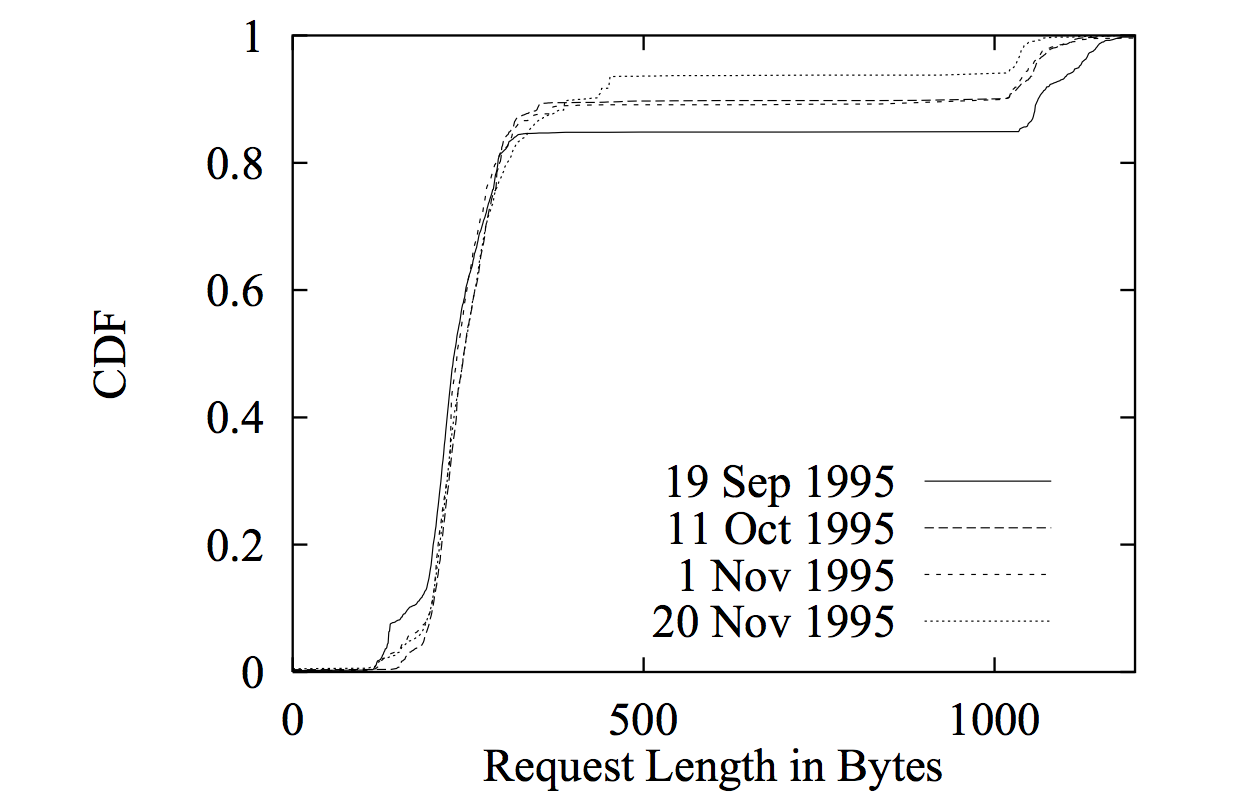
\includegraphics[scale=0.3]{histogram1.png} & 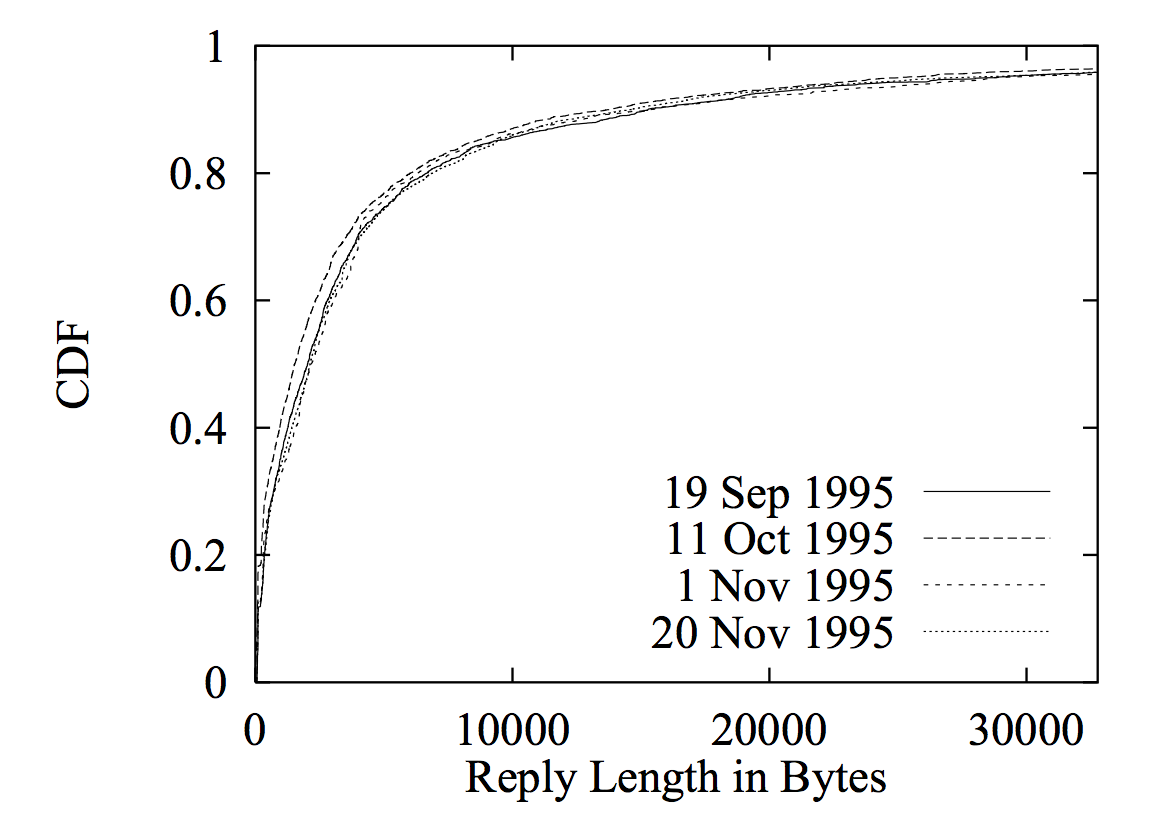
\includegraphics[scale=0.3]{histogram2.png} \\
\multicolumn{2}{c}{Distribution of web traffic request and reply sizes, respectively \cite{mah1997empirical}.}
\end{tabular}
\end{center}
\label{fig:histogram1}
\end{figure*}

\noindent
\textbf{Video Streaming Traffic:} Video streaming traffic as described in \cite{badia2010markov} is composed of two types of packets -- I and D packets -- each of which are tightly correlated and with different characteristics. Video segments are sent in sets of I and D packets, wherein multiple small D packets carrying video data are dependent on a single I packet with metadata necessary to decode the video stream. The length of each I and D packet is correlated to past packet lengths. For example, let $\lambda_j(t|s)$ denote the probability that a packet of type $j \in \{I ,D \}$ is $t$ time slots long given that the previous packet of type $j$ was $s$ packets long. The size of both I and D packets are bounded within a finite range so as to make the analytical model tractable. 

In this work we consider a more specific type of multimedia encoding scheme, namely, MPEG. MPEG video traffic streams consist of I, P, and B packets \cite{sony-demo}. In this case, a single I frame is transmitted, is an intraframe and is heavily coded (thus, larger) to ensure it can be correctly decoded by all receivers. P frames follow the I frame, and are used to transmit actual multimedia data. These rely on the previous I frame and P frames to be decoded correctly. B frames -- bidirectional frames -- are transmitted in between I and P frames and naturally serve to relay information in both directions. 

\begin{figure*}
\begin{center}
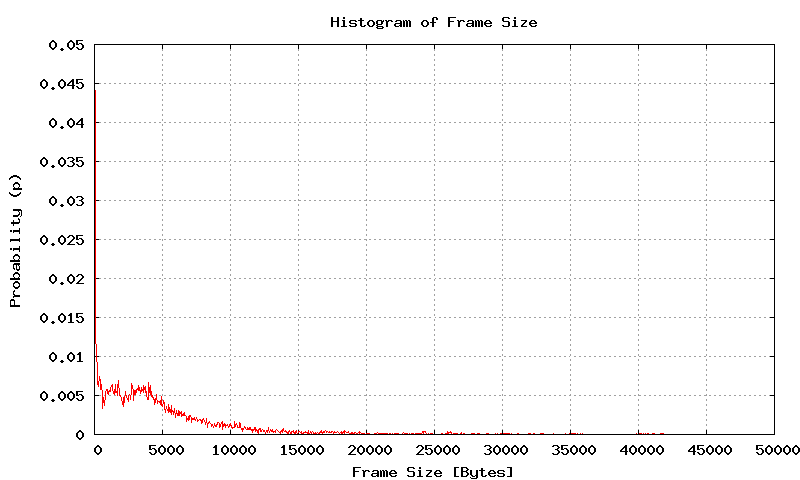
\includegraphics[scale=0.35]{frame.png}
\caption{Distribution of multimedia frame sizes \cite{sony-demo}.}
\label{fig:frame}
\end{center}
\end{figure*}

\begin{figure*}
\begin{center}
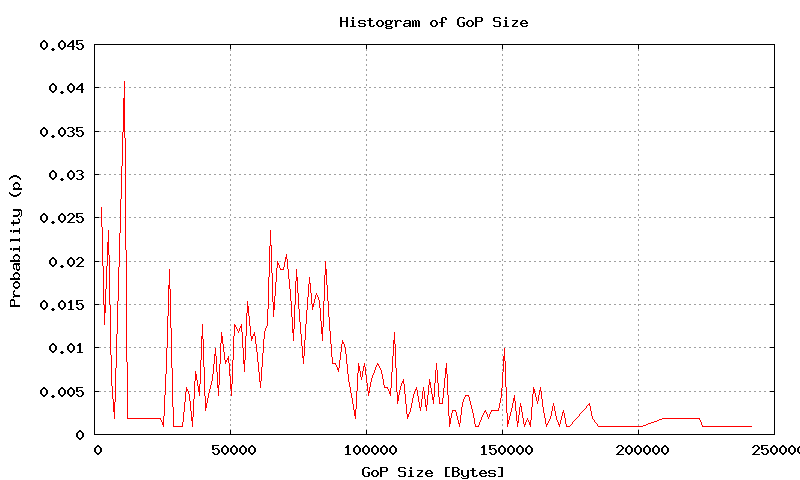
\includegraphics[scale=0.35]{gop.png}
\caption{Distribution of GoP sizes in multimedia traffic \cite{sony-demo}.}
\label{fig:gop}
\end{center}
\end{figure*}

To further understand the differences between these types of traffic, we used our simulator to generate system state transition traces in the context of a simulator. The results of these traces are shown in Figure \ref{fig:traces}. Note that the superposition all traces, shown in the bottom Figure, is the object of study in this work. Namely, we seek to understand the behavior of the DCF as it serves packets generated from sources of heterogeneous traffic.

\begin{figure*}
\begin{tabular}{cc}
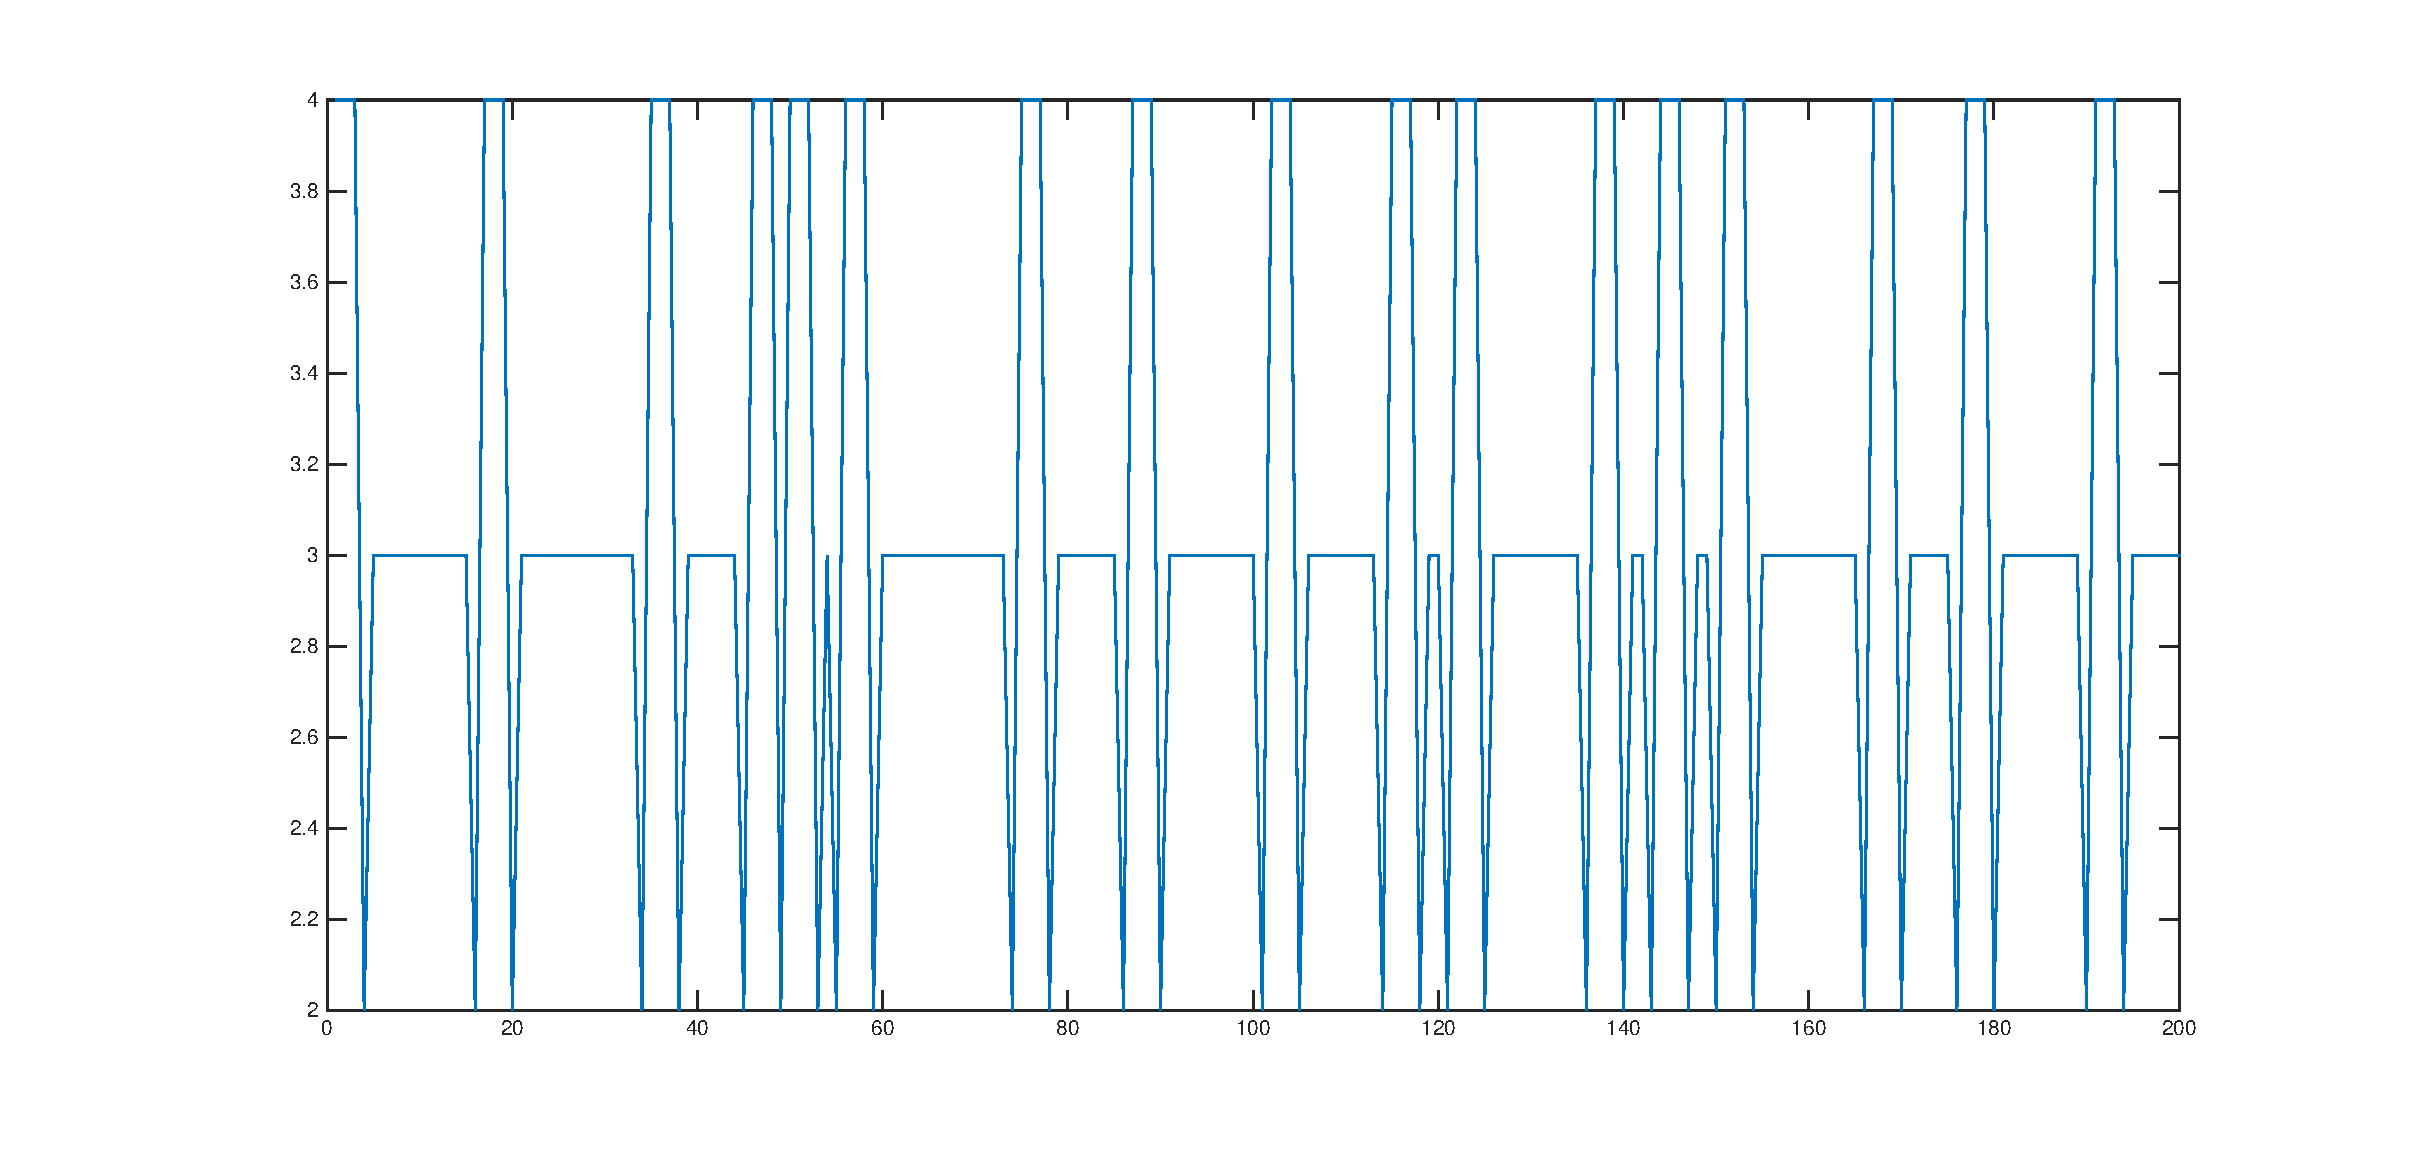
\includegraphics[width=\textwidth,height=100px]{../../src/results/browse_time.eps} \\
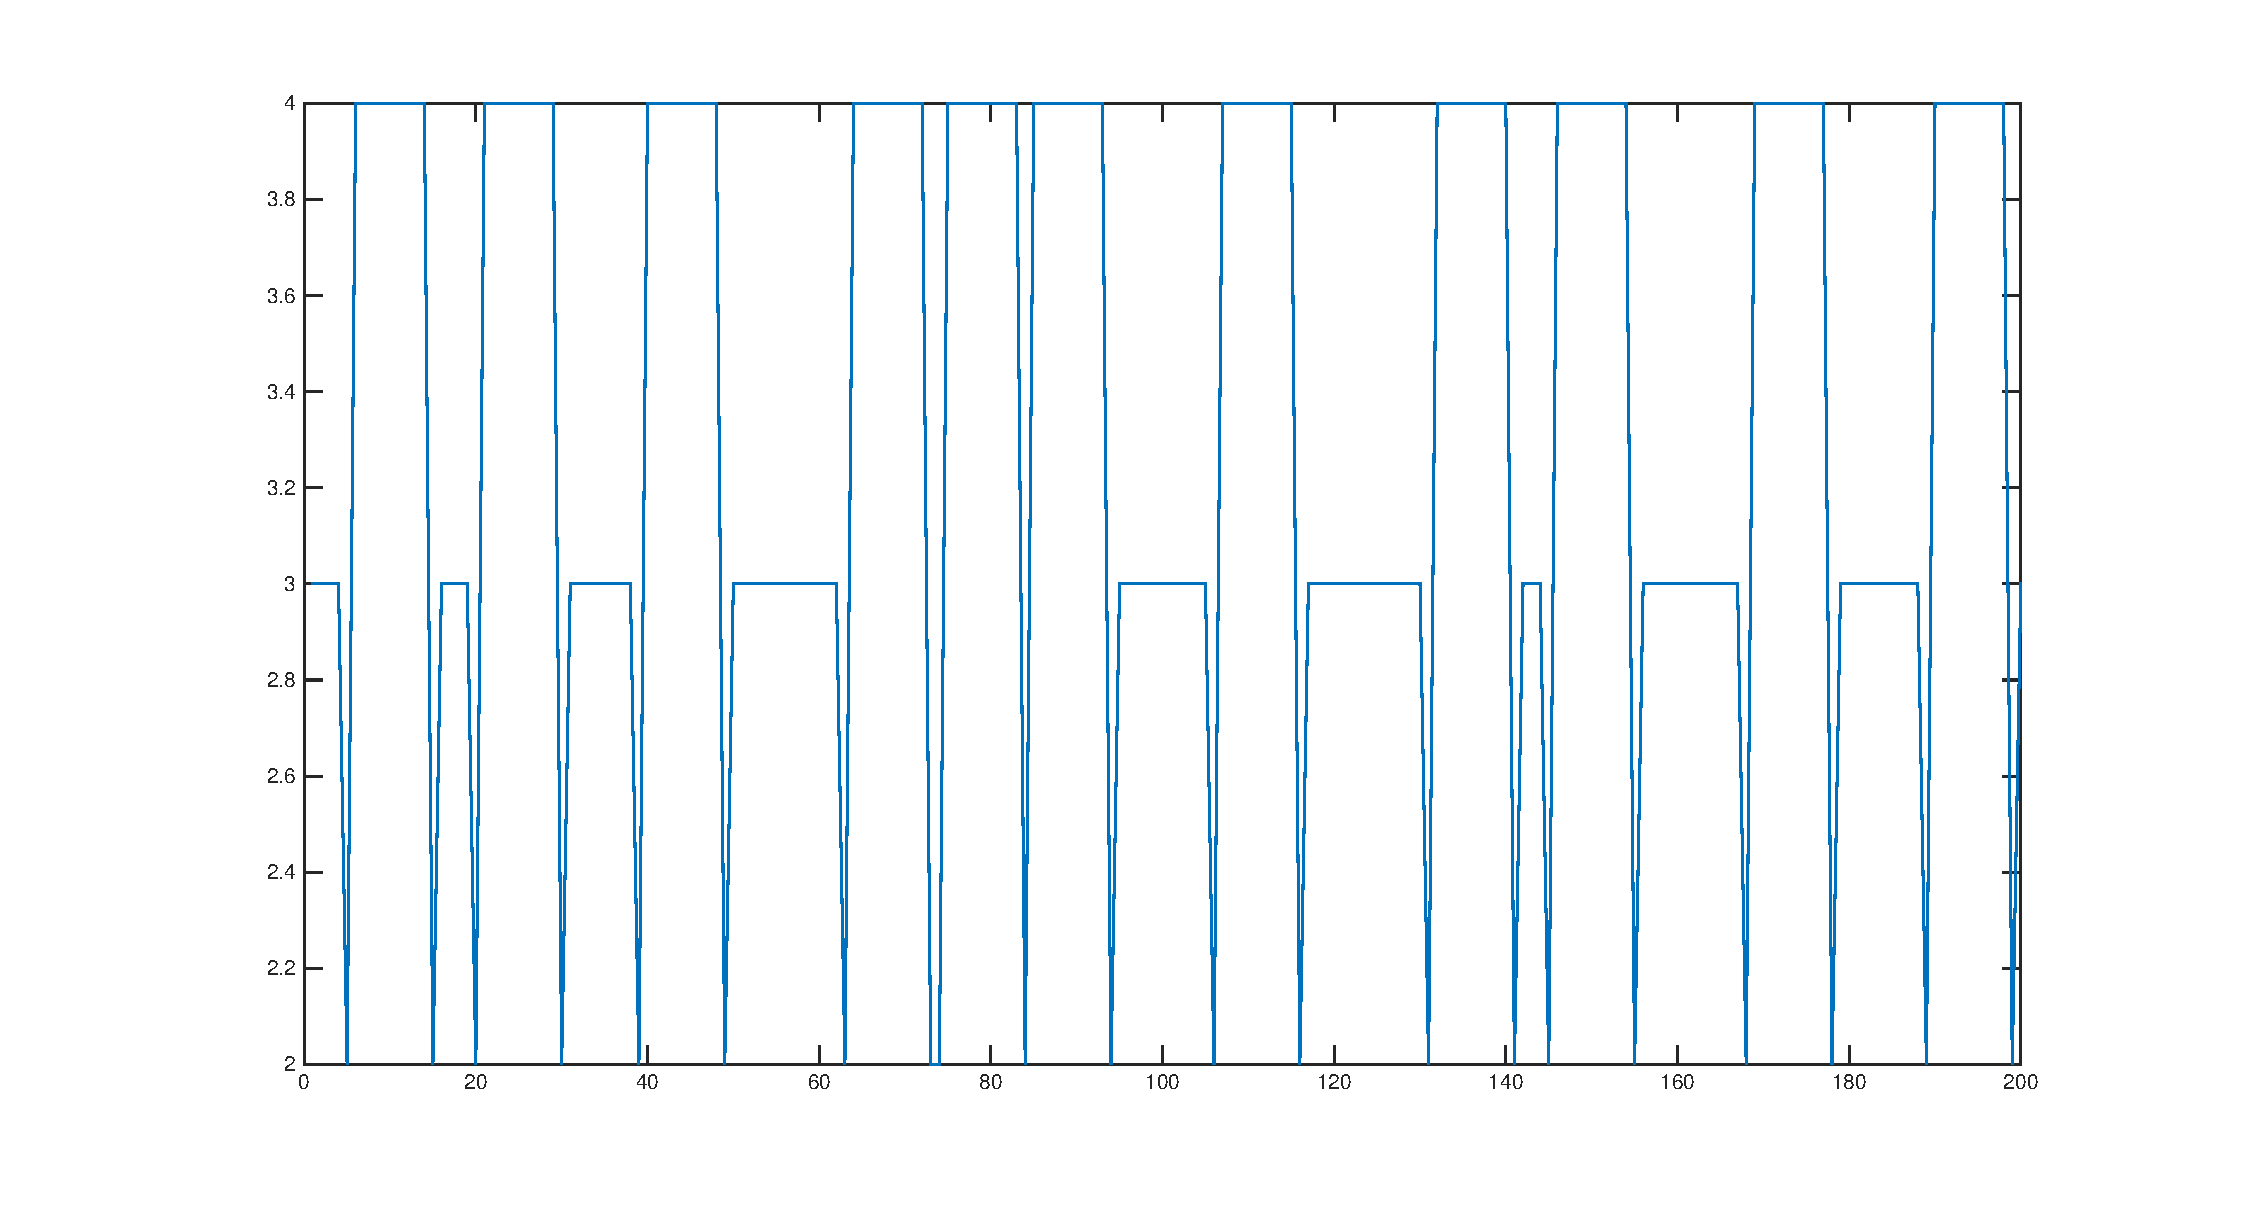
\includegraphics[width=\textwidth,height=100px]{../../src/results/file_time.eps} \\
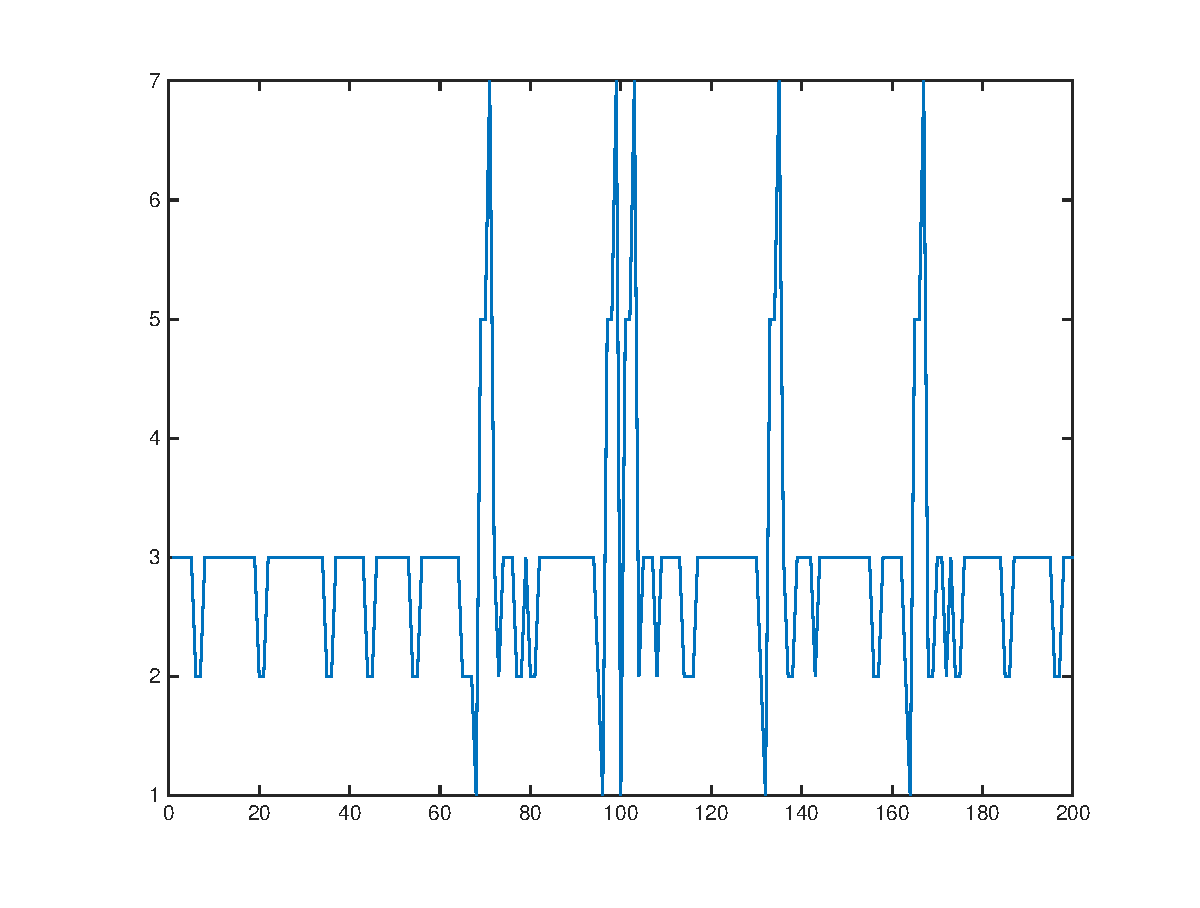
\includegraphics[width=\textwidth,height=100px]{../../src/results/video_time.eps} \\
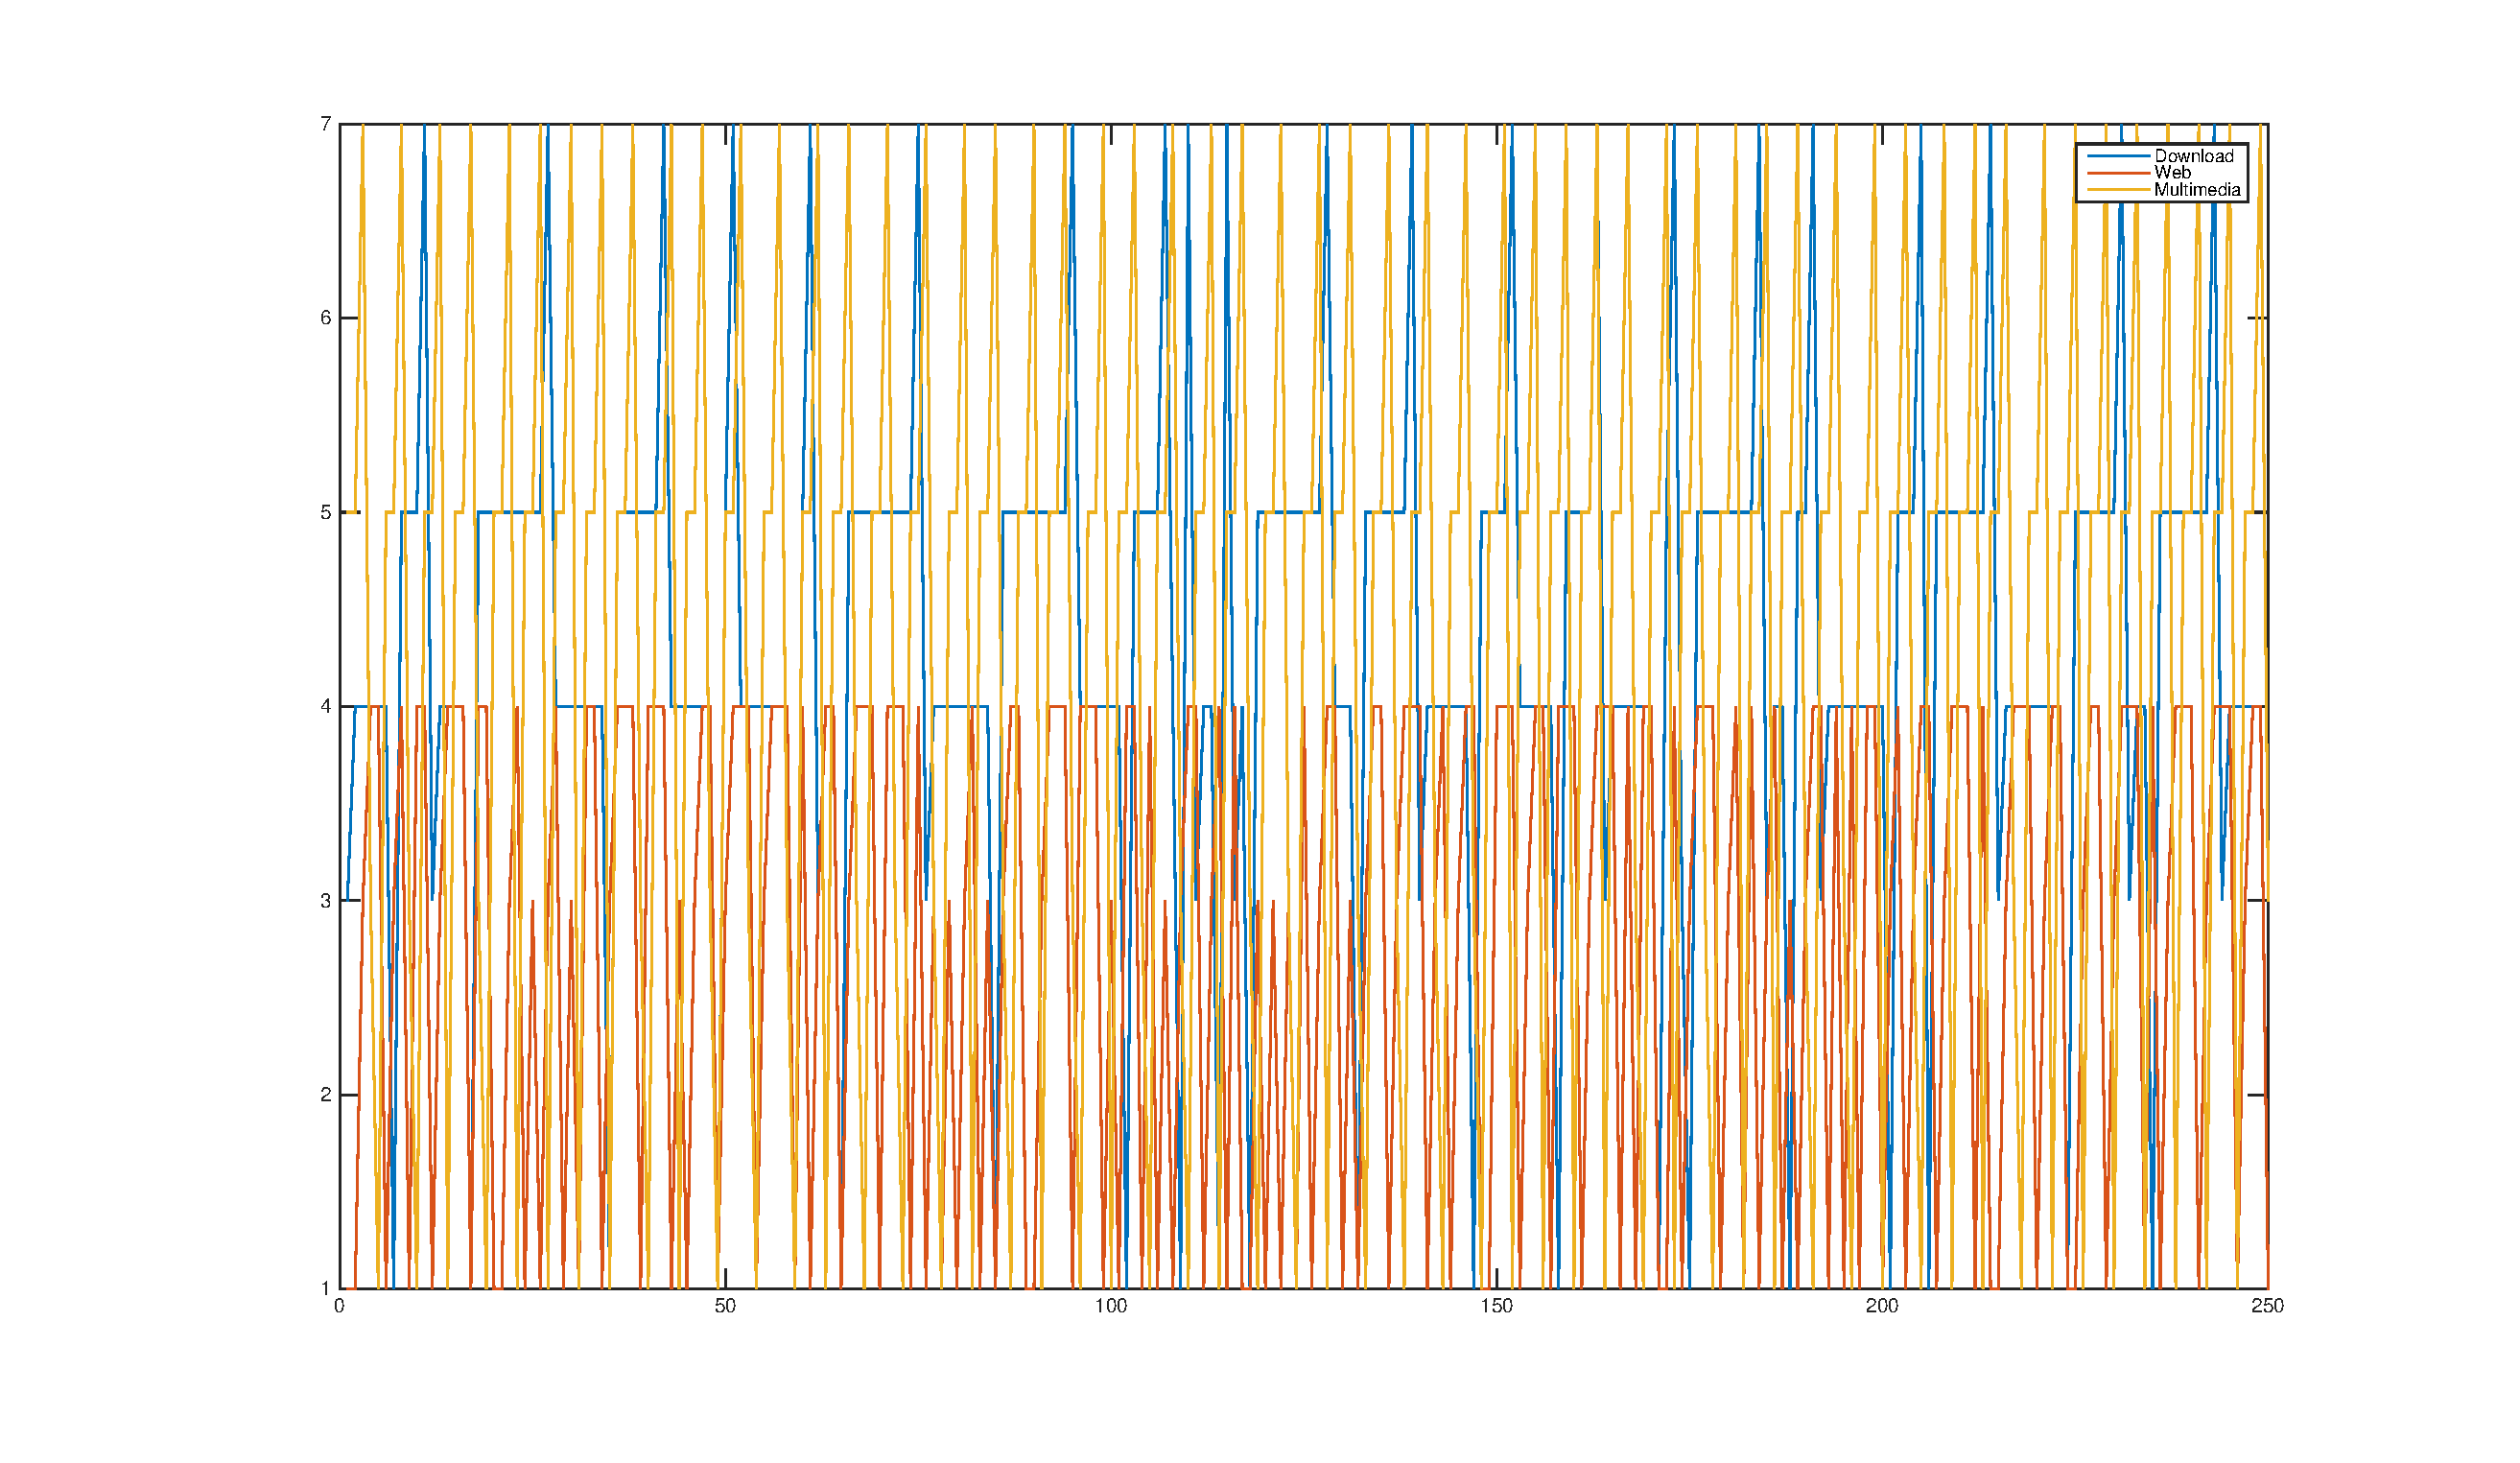
\includegraphics[width=\textwidth,height=100px]{../../src/results/all.eps} \\
\end{tabular}
\caption{Individual system transition traces for (1) web browsing, (2) file download, and (3) video streaming traffic. The bottom trace shows the superposition of all the above traces. The $x$ axis is the discrete time in the system, and the $y$ axis is the state. For completeness, state $5$ is interarrival, $4$ is the packet size calculation, $3$ is a waiting state (e.g., backoff, postbackoff), $2$ is a failure transmission, and $1$ is a successful transmission.}
\label{fig:traces}
\end{figure*}

We will use the characteristics of each of these models to tune our Markov models in the experimental section of this report. 

\section{The 802.11 Distributed Control Function}
The 802.11 DCF \cite{ieee1997wireless} is at the core of this work. It is a simplistic random access scheme based on the carrier sense multiple access with collision avoidance (CSMA/CA) protocol. Failed packets are retried according to a binary exponential backoff rule. At each packet transmission, the backoff is uniformly in the range ($0, w-1$), where $w$ is the length of the ``contention window'' and is directly dependent on the number of failed attempts for the packet thus far. The window $w$ is set to $W_{min}$ to begin, and upon every failure, the backoff counter is doubled. At stage $i$, the backoff timer is $2^iW_{min}$. The maximum backoff is bounded by $W_{max} = 2^mW_{min}$. Selections of $W_{min}$ and $W_{max}$ are dependent upon the physical layer specifications in the 802.11 standard \cite{ieee1997wireless,dcf}. For example, frequency hopping spread spectrum calls for $W_{min} = 16$ and $W_{max} = 1024$ ($m = 6$). 

\section{Incremental Markov Models for Heterogeneous Traffic}
In this section we describe the necessary evolutions of Bianchi's original Markov model to support parameterized packet length, interarrival time, and buffer saturation. Ultimately, the extensions enable us to parameterize the following characteristics: interarrival time, packet size, probability of a new packet arriving (i.e., buffer saturation), and the probability of a node waiting for a non-zero interarrival time. The usage of these parameters to emulate web browsing, file downloads, and multimedia traffic is elaborated upon in Section \ref{sec:experiment}.

\subsection{Original DCF Model}
A simple Markov model for the 802.11 DCF function was proposed in the seminal work by Bianchi \cite{dcf}. The system state is described by two discrete-time stochastic processes $b(t)$ and $s(t)$: $b(t)$ represents the backoff \emph{time counter} and $s(t)$ represents the backoff \emph{stage} for a given station or node, each of which is advanced at each time step (i.e., from $t$ to $t + 1$). Each node is equipped with a \emph{saturated} buffer of packets to transmit; there is never a case where a node has to wait for a packet to arrive in the buffer before attempting a transmission. Also, instead of modeling multiple nodes simultaneously to accurately assess the probability of collision, this model assumes a constant probability of collision $p$ -- the conditional collision probability -- at each time slot. In the real world, this probability is a function of the network and environmental interferences, e.g., shadowing, fading, etc. However, by making this a constant and therefore independent from other nodes, the model simplifies to capturing the dynamics of the bidimensional process $\{ b(t), s(t) \}$ as a discrete-time Markov chain, shown in Figure \ref{fig:dcf_model}. 

The only non-null transition probabilities in this Markov chain are given below:

\begin{center}
\begin{math}
\boxed{
\begin{array}{lll}
\Pr[i,k | i, k + 1] = 1, & k \in [0, W_i - 2], & i \in [0,m] \\
\Pr[0,k | i, 0] = (1-p)/W_0, & k \in [0, W_0 - 1], & i \in [0,m] \\
\Pr[i,k | i-1, k] = p/W_i, & k \in [0, W_i - 1], & i \in [1,m] \\
\Pr[m,k | m,0] = p/W_m, & k \in [0, W_m - 1] & ~
\end{array}
}
\end{math}
\end{center}

\begin{figure*}
\begin{center}
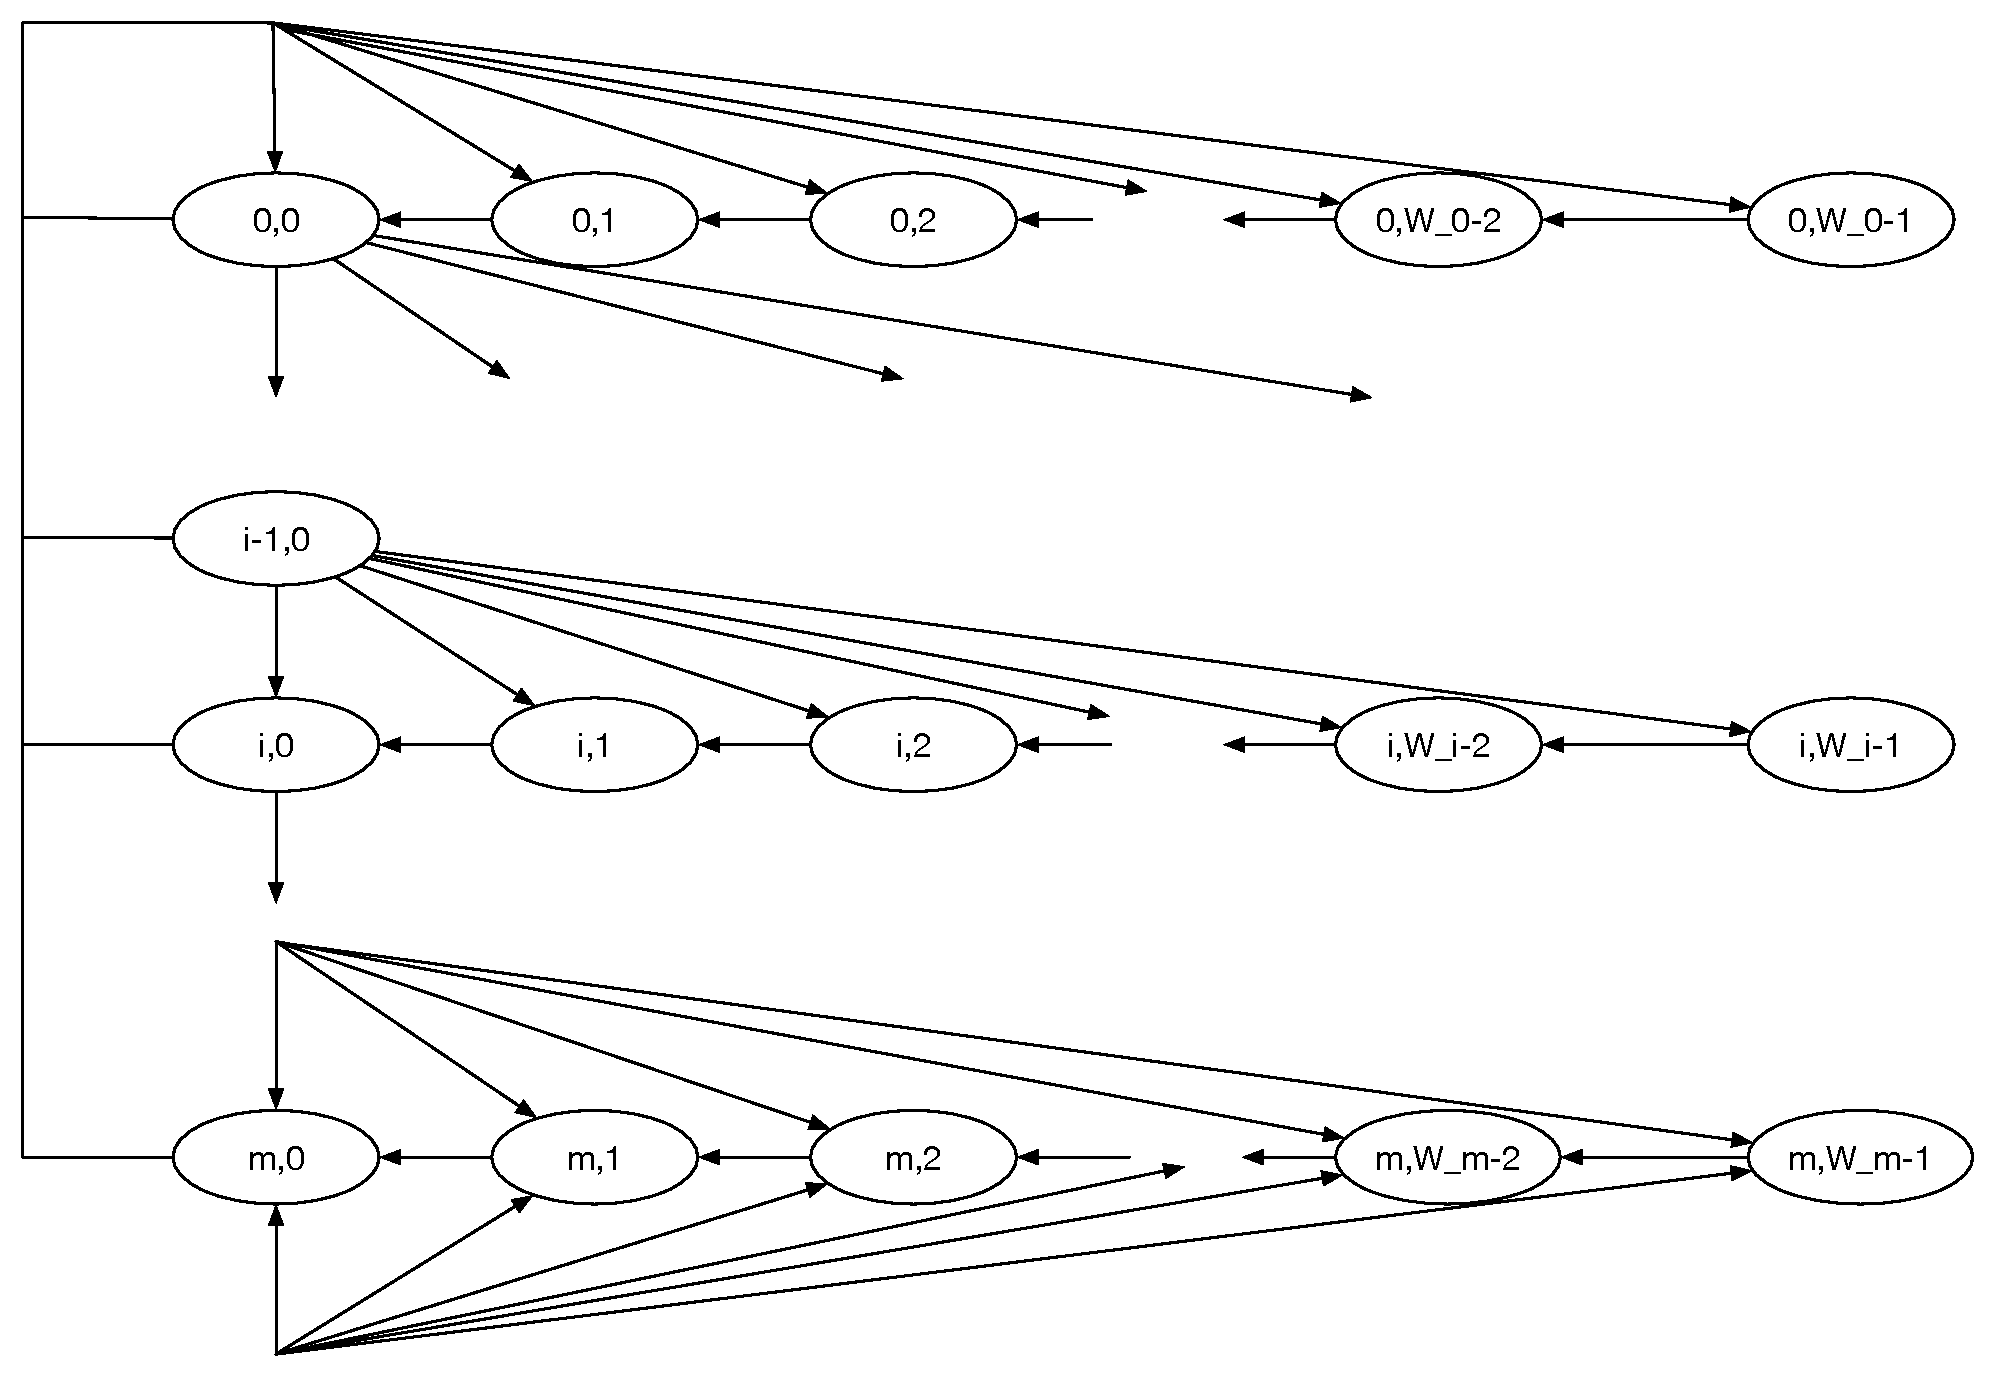
\includegraphics[scale=0.35]{../../sketches/dcf_model.pdf}
\caption{The original saturated DCF Markov model \cite{dcf}.}
\label{fig:dcf_model}
\end{center}
\end{figure*}

\subsection{Limited and Diverse Traffic} \label{sec:nonsaturated}
While accurate, the original DCF model is constrained in that it assumes homogeneous traffic and a saturated stream of packets for transmission. Malone et al. \cite{dcf-nonsaturated} presented a modified version of Bianchi's model that captures non-saturated traffic loads. The essential idea behind their variant is that there exists a constant packet arrival probability $q$ at each time slot, much like there exists a constant collision probability $p$. If a node successfully transmits a packet and the buffer is not-empty, the state of the system proceeds as normal. Conversely, if a packet is not ready for transmission, then the chain enters a stage known as ``postbackoff,'' denoted $(0,k)_e$ for $k \in [0, W_0-1]$. A node may remain in this set of states indefinitely until a packet arrives and the channel is idle.

To capture the mechanics of the DCF function in this condition, the postbackoff set of stages are nearly indentical to backoff stage $i = 0$. If a packet arrives at any time when the system is in a postbackoff state, it immediately transitions into the backoff stage $i = 0$, with a decremented backoff timer. However, if the postbackoff timer reaches $0$, where the postbackoff is said to be complete, the node will stay in this state until a packet arrives with probability $q$. Once a packet arrives in state $(0, 0)_e$ with probability $q$, there are three possible outcomes: (1) the packet is transmitted successfully, a collision occurs with probability $p$, or the medium (channel) is sensed as busy with probability $1 - P_{idle} = p$. 

With the addition of the postbackoff states $S'$, the Markov chain itself is now a multidimensional process $\{b(t), s(t), S' \}$. The new state transition probabilities needed to capture the transitions between these multiple dimensions are below.

\begin{center}
\begin{math}
\boxed{
\begin{array}{lll}
\Pr[(i,k-1) | (i, k)] = 1 & k \in [1, W_i-1] & i \in [1,m] \\
\Pr[(0,k-1)_e | (0, k)_e] = 1-q & k \in [1, W_i-1] & i \in [1,m] \\
\Pr[(0,k-1) | (0, k)_e] = q & k \in [1, W_i-1] & i \in [1,m] \\
\Pr[(0,k)_e | (i, 0)] = \frac{(1-p)(1-q)}{W_0} & k \geq 0 & i \in [0,m] \\
\Pr[(0,k) | (i, 0)] = \frac{(1-p)q}{W_0} & k \geq 0 & i \in [0,m] \\
\Pr[(\max\{(i+1,m\}, k) | (i, 0)] = \frac{p}{W_{\max\{i+1,m\}}} & k \geq 0 & i \in [0,m] \\
\Pr[(0,0)_e | (0, 0)_e] = 1 - q + \frac{qP_{idle}(1 - p)}{W_0} & ~ \\
\Pr[(0,k)_e | (0, 0)_e] = \frac{qP_{idle}(1 - p)}{W_0} & k > 0 \\
\Pr[(1,k) | (0, 0)_e] = \frac{qP_{idle}p}{W_1} & k \geq 0 \\
\Pr[(0,k) | (0, 0)_e] = \frac{q(1 - P_{idle})}{W_0} & k \geq 0 \\
\end{array}
}
\end{math}
\end{center}

\begin{figure*}
\begin{center}
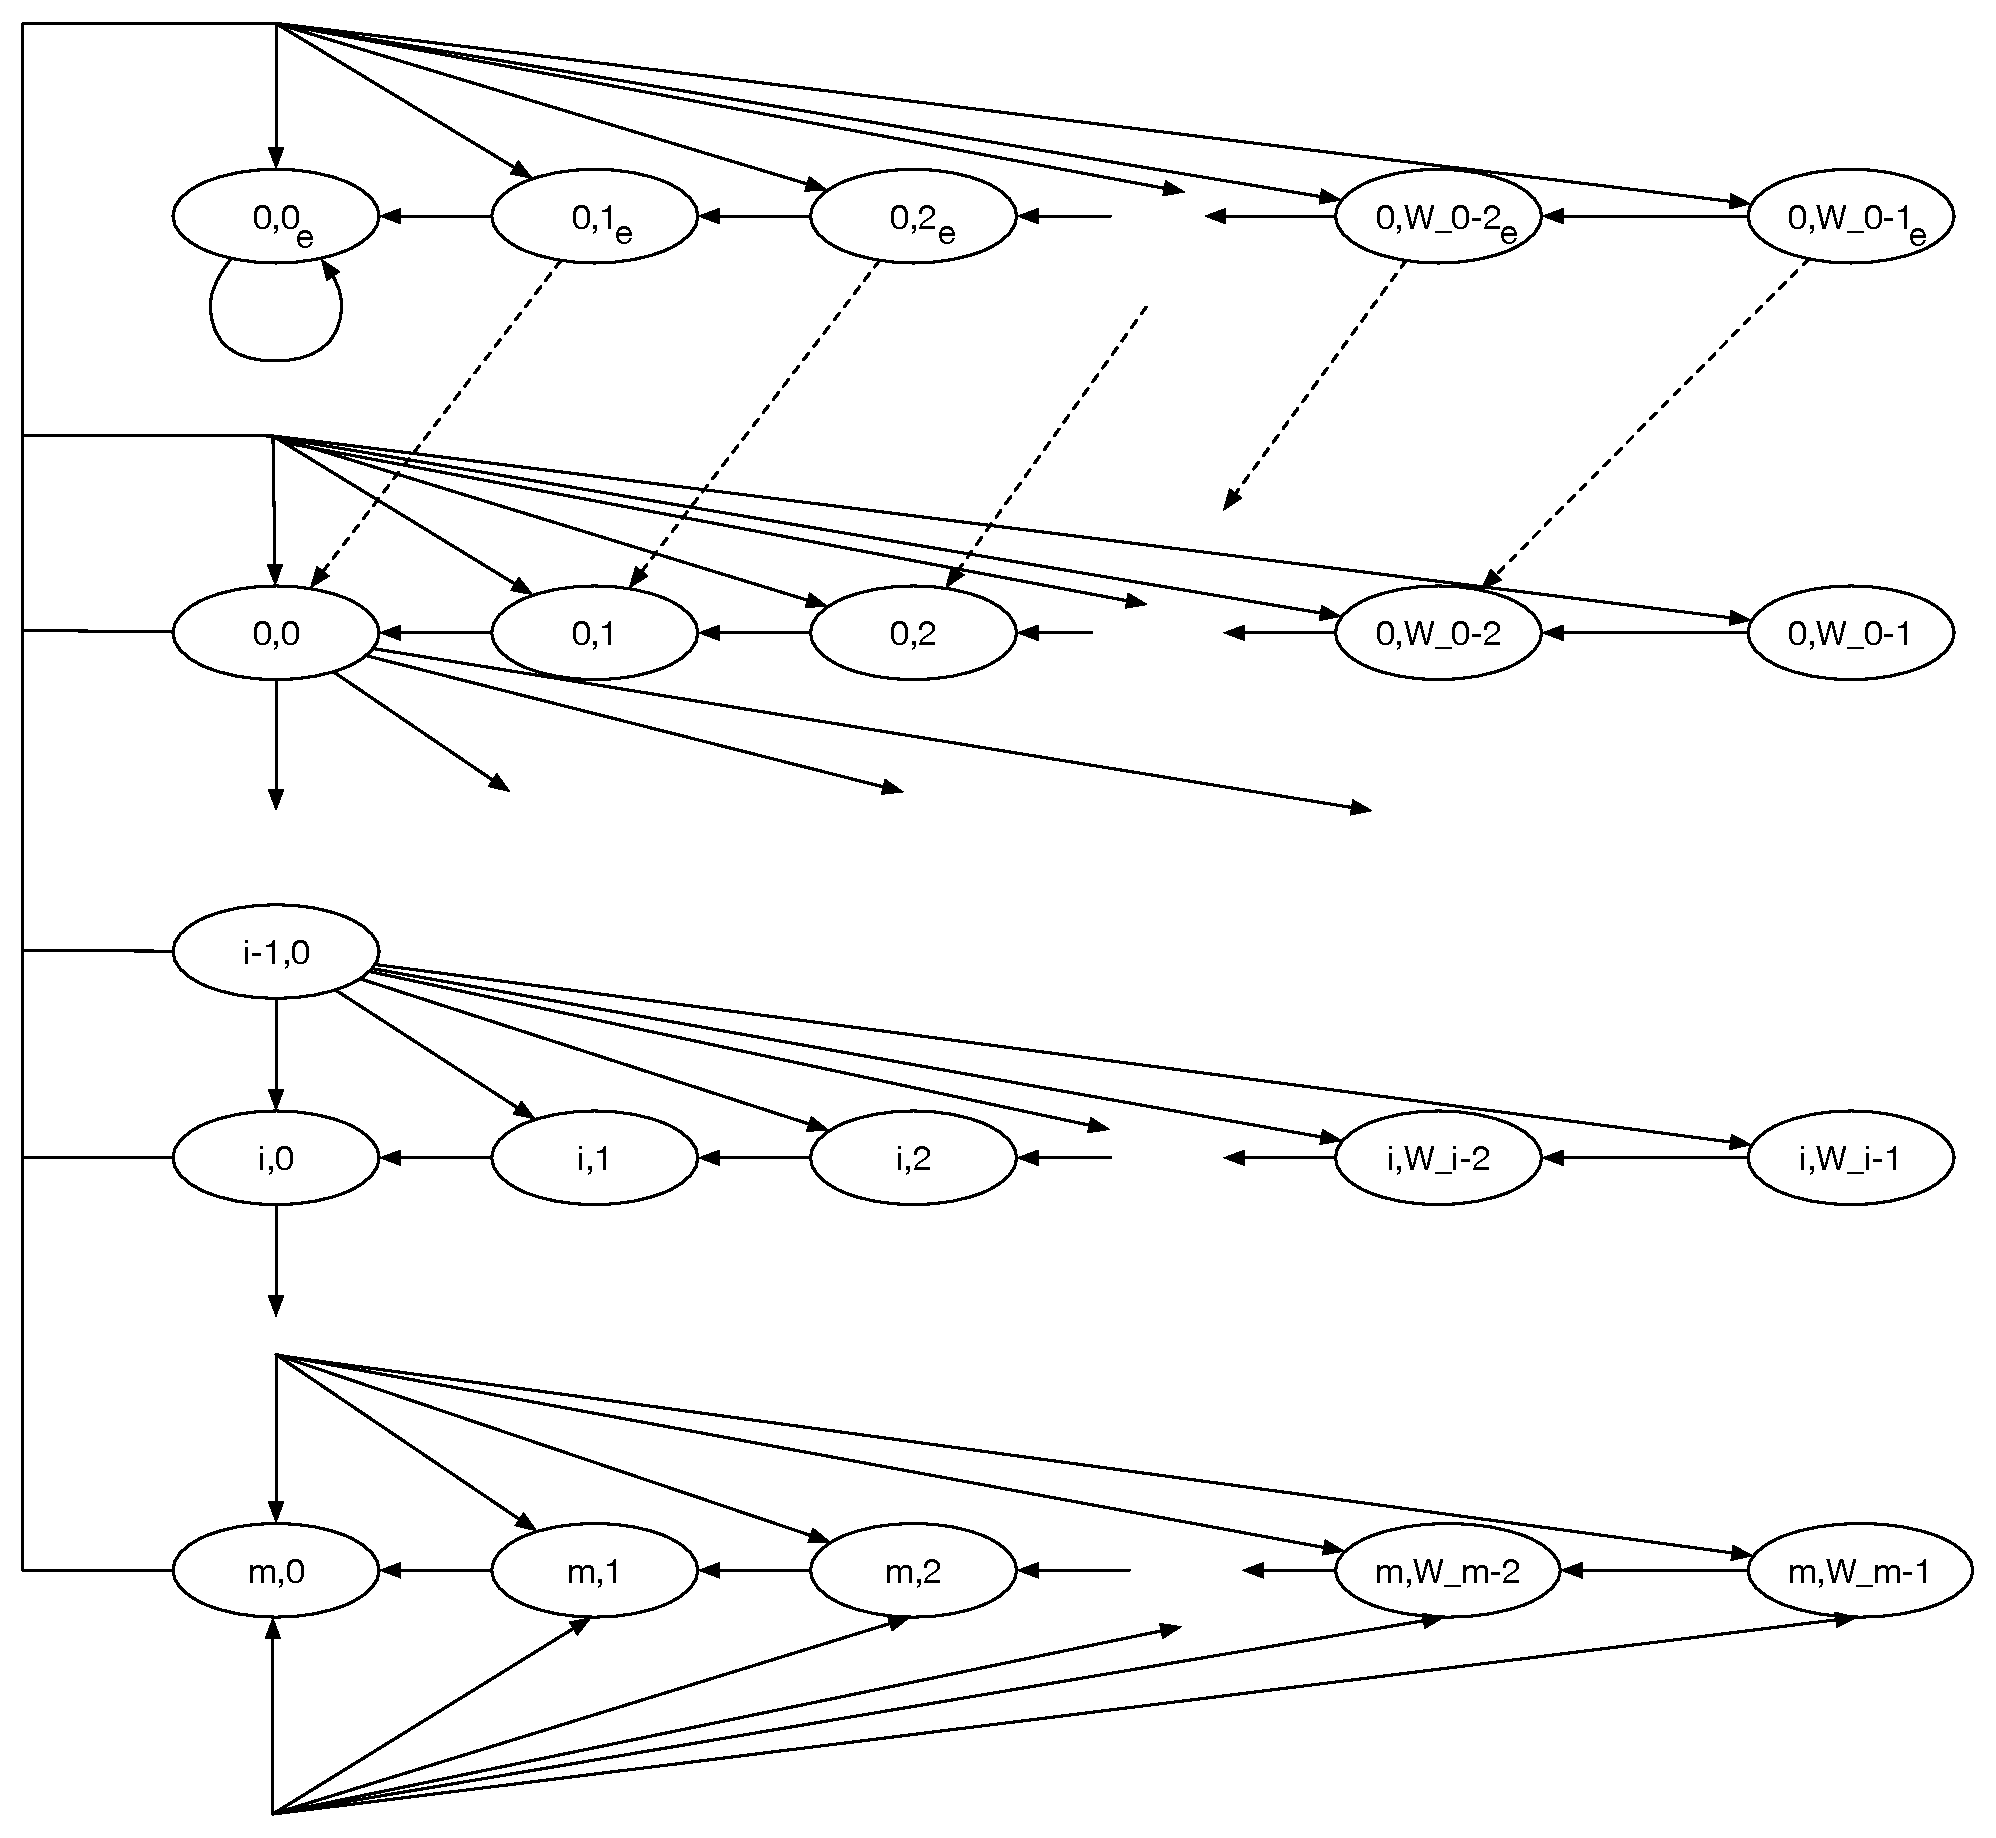
\includegraphics[scale=0.35]{../../sketches/dcf_model_nonsaturated.pdf}
\caption{The modified DCF Markov model that captures non-saturated traffic \cite{dcf-nonsaturated}.}
\label{fig:dcf_model_nonsaturated}
\end{center}
\end{figure*}

Malone et al. \cite{dcf-nonsaturated} exploited the inclusion of this postbackoff state and the fixed arrival probability constant to study the performance of the DCF while transferring packets from unsaturated heterogeneous traffic, e.g., file downloads, web traffic, etc. However, their analysis was limited in scope, since heterogeneous traffic types were parameterized only by $p$ and $q$.

\subsection{Adding Variable Length Frame Payloads}
Despite the flexibilty in the previous model, it is still limited with respect to packet size. In particular, the model assumes that each packet has an equally sized payload. This is not true, especially for video traffic \cite{badia2010markov}, which typically consists of two types of packets of distinctly different sizes: $d$ packets are small video frame/segment packets that carry information needed to render a piece of video data, and $i$ packets are large ``metadata'' packets that contain information necessary to decode $d$ packets. Multiple $d$ packets are often tied to a single $i$ packet in such a way that if the $i$ packet is lost, none of its children $d$ packets can be decoded correctly. Consequently, we need to be able to model packets of different sizes. 

To do this, we consider a range of possible packet sizes, e.g., $[1,l]$, where $l$ is the maximum packet payload size. In this context, the packet size corresponds to \emph{how many} discrete time slots are needed to transfer the content over the channel. In the previously two discussed models, the packet size was assumed to be $1$ since they were assumed to be transferred in a single time step. Since we may want to support both deterministic and arbitrary packet sizes, drawn from a specific distribution, we use what we call size chain blackboxes to capture this type of variability. Figure \ref{fig:size_chain} shows a sample size chain blackbox for the range of values $[1,4]$. There are $l$ ($l = 4$) transitions into the blackbox, and each transition $l'$ is to a chain of length $l'$. 

\begin{figure}
\begin{center}
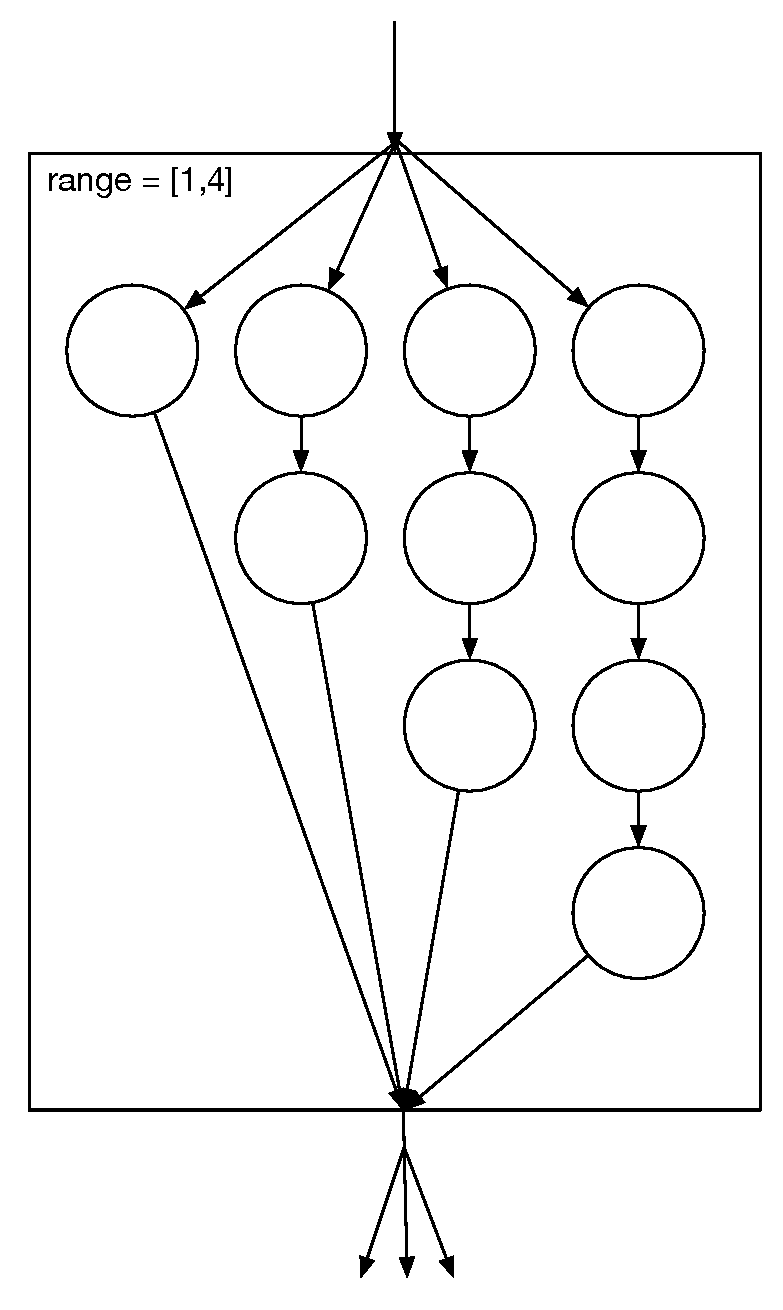
\includegraphics[scale=0.35]{../../sketches/size_chain_old.pdf}
\caption{A blackbox Markov chain that captures bounded variabilities in a particular parameter, such as packet length or packet interarrival time.}
\label{fig:size_chain}
\end{center}
\end{figure}

To show how this chain would be used, assume that the size chain blackbox represents the size of a particulr packet. Further, assume that the packet size is a discrete random variable ranging from 1 to 4 with uniform distribution. The probability of transferring to any chain within the blackbox from the entry state is $(1/4)$. If the transition was to the last chain of length $l = 4$, then the state would appear to ``loop'' in place for 4 time steps before exiting the blackbox. Conversely, if the transition was to the first chain of length $l = 1$, then the state would only loop once before exiting. Although these states are costly from the persepctive of space, this type of construction enables us to model such discrete random variables with any distribution within our Markov chain. 

The first application of these size chain blackboxes are to extend the previously discusssed nonsaturated model to support variable packet sizes. Specifically, the number of time steps needed to transfer a packet and detect collision is now a bounded discrete random variable. This means that once a packet has begin transmitting it enters a size chain blackbox before either (a) detecting collision or (b) completing successfully. It is important to note that for packets of length $l > 1$, the probability of a collision is no longer $q$. Rather, a collision occurs if there is a collision in \emph{any} time slot during which the packet was being transmitted. This means that the probability of collision for a packet of length $l$ is $1 - (1 - p)^l$. 

The new states required to model the size chain blackboxes are tuples of the form $(i, l, l')$, where $i$ is the backoff stage and $l$ is the packet length, and $l'$ is the \emph{state} within the size chain of length $l$. For example, if the state transitions into a size chain of length $l = 4$ from state $(i, 0)$, then the following series of transitions would occur: 
\begin{align*}
(i, 4, 4) & \to (i, 4, 3) \\
& \to (i, 4, 2) \\
& \to (i, 4, 1)
\end{align*}

To model this behavior, which is visually shown in Figure \ref{fig:dcf_model_unsaturated_varpktsize}, the following new state transition probabilities are included into the model:

\begin{center}
\begin{math}
\boxed{
\begin{array}{lll}
\Pr[(i,l,l'-1) | (i,l,l')] = 1 & l' \leq l & l' \geq 0 \\
\Pr[(i+1,k) | (i,l,0)] = \frac{1 - (1 - p)^l}{W_{i+1}} & ~ & k \in (0, W_{i+1} - 1) \\
\Pr[(0,k) | (i,l,0)] = \frac{(1 - q)(1 - p)^l}{W_0} & ~ & k \in (0, W_{0} - 1) \\
\Pr[(0,k)_e | (i,l,0)] = \frac{q(1 - p)^l}{W_0} & ~ & k \in (0, W_{0} - 1) \\
\end{array}
}
\end{math}
\end{center}

\begin{figure*}
\begin{center}
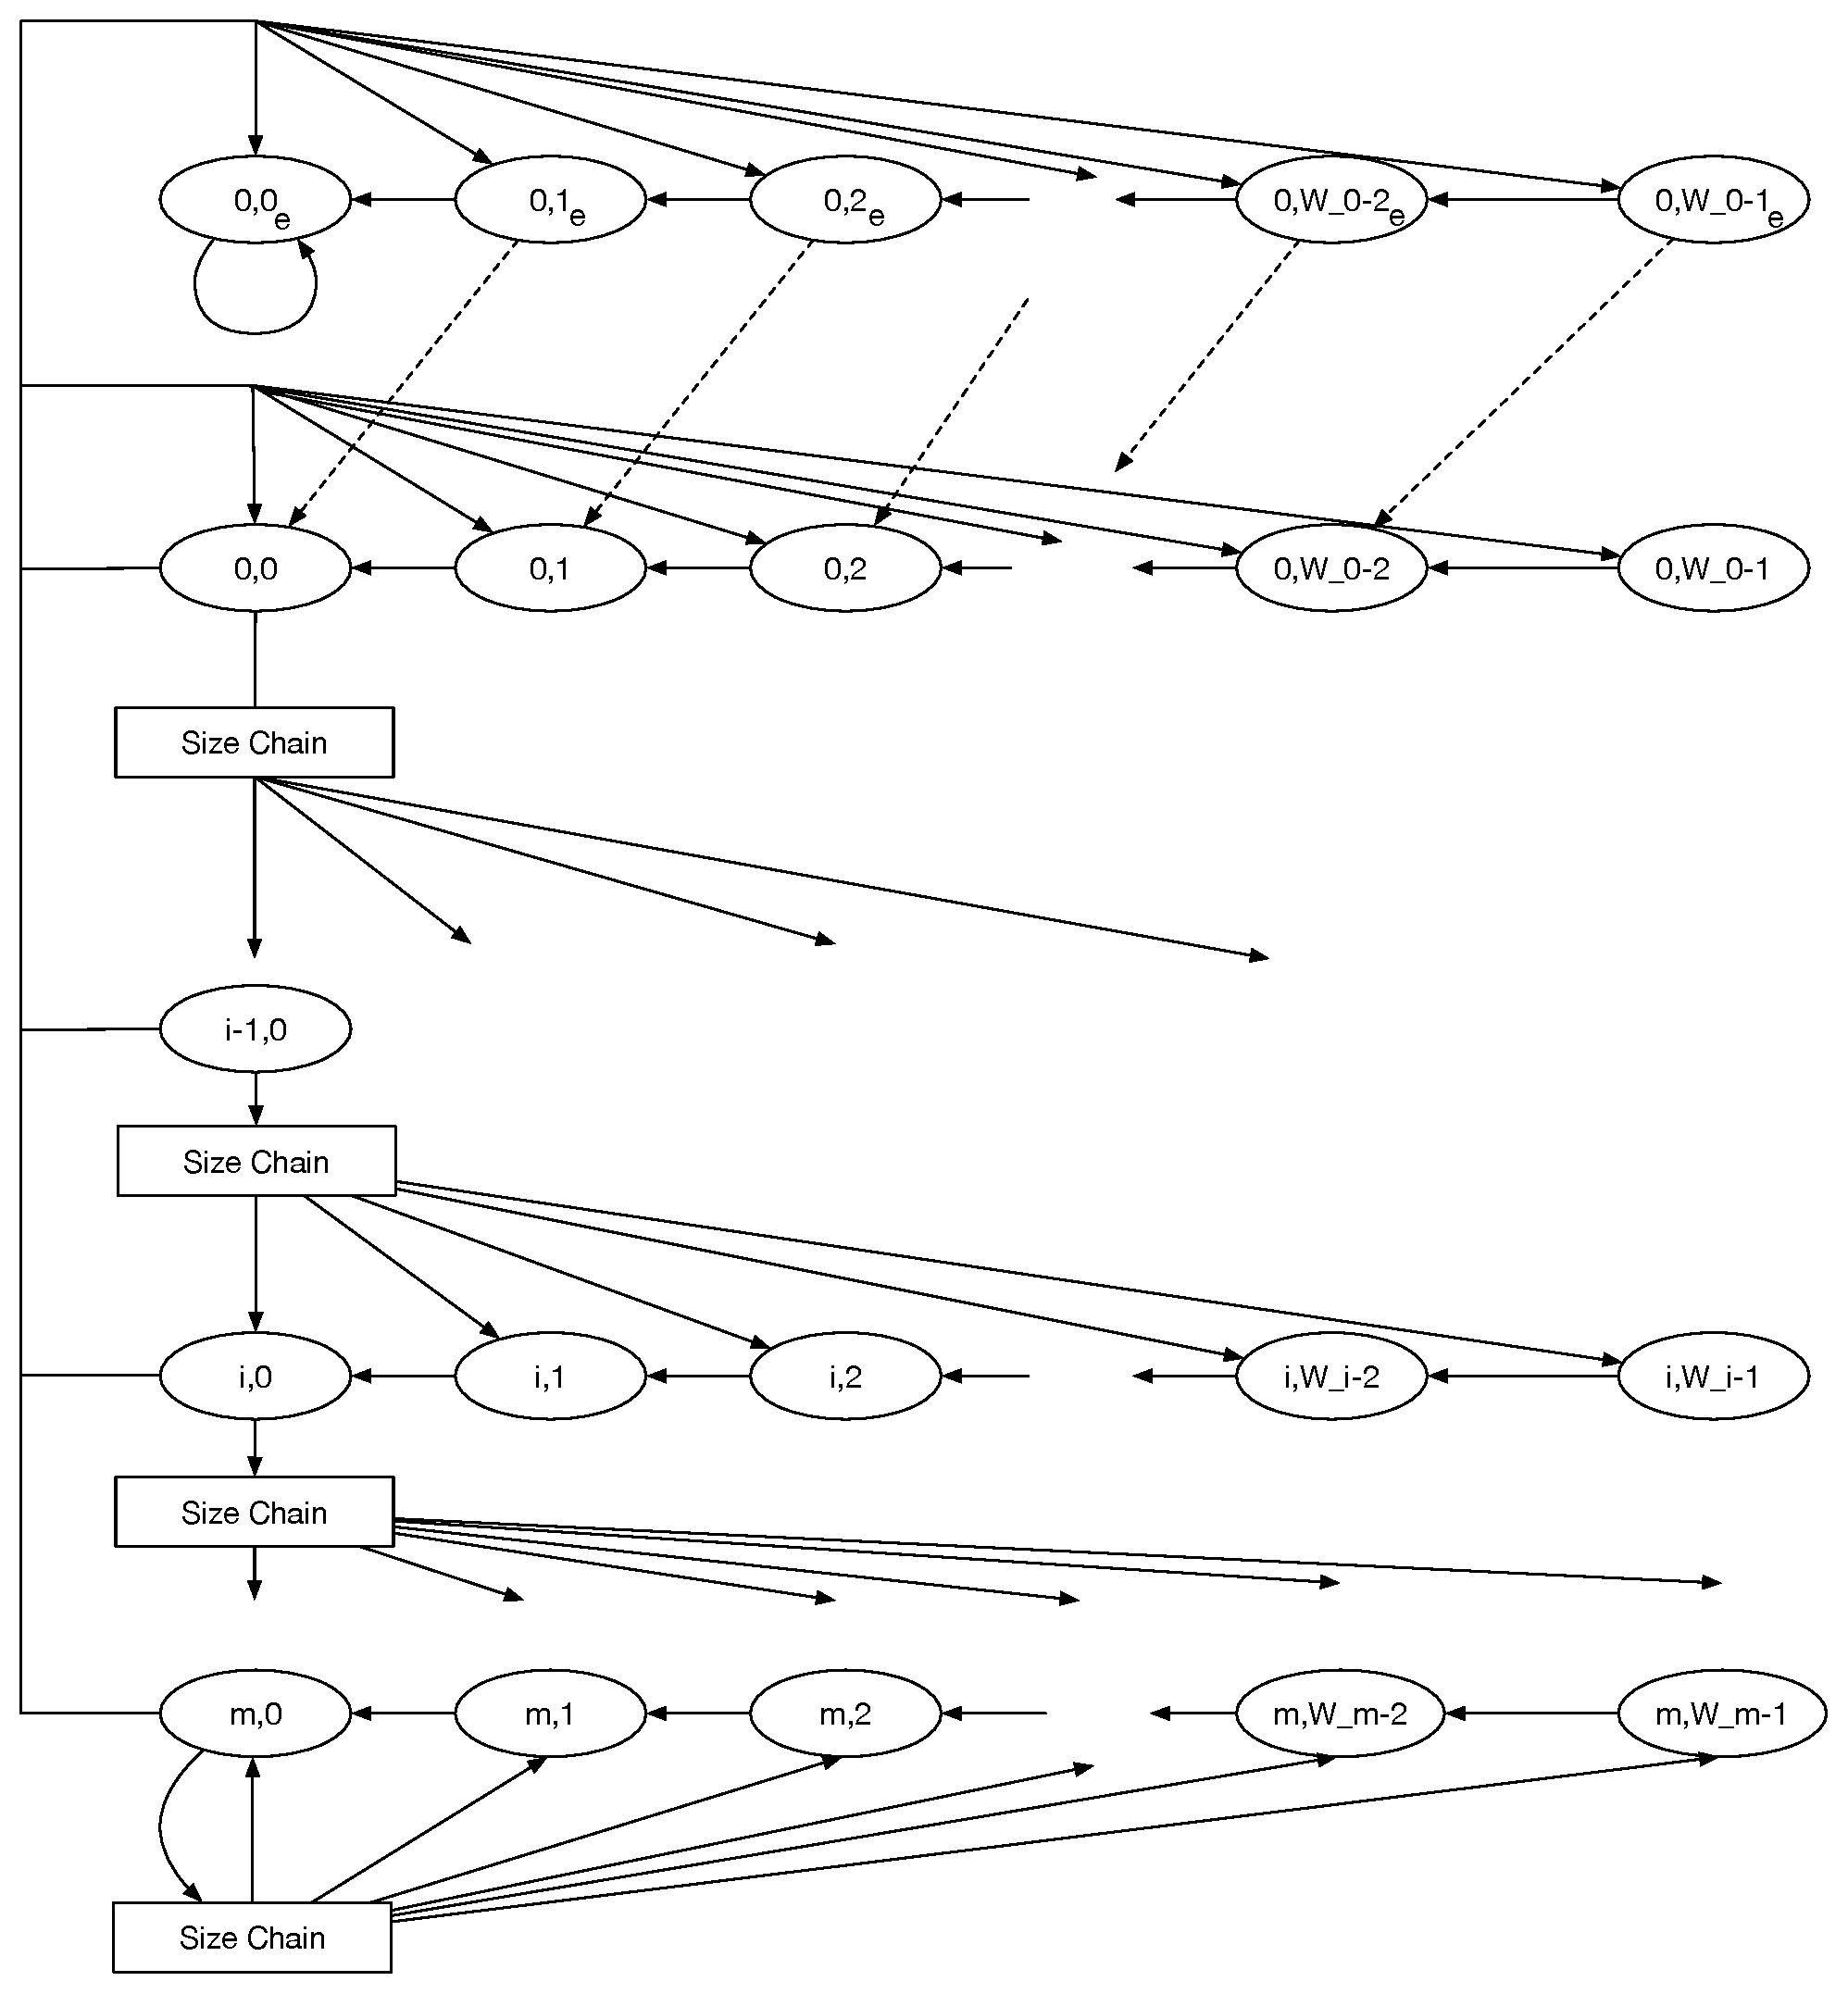
\includegraphics[scale=0.35]{../../sketches/dcf_model_unsaturated_varpktsize.pdf}
\caption{The modified unsaturated DCF Markov model that captures variable-length packet payloads.}
\label{fig:dcf_model_unsaturated_varpktsize}
\end{center}
\end{figure*}

\subsection{Adding Arbitrary Inter-Arrival Times}
The final extension of our Markov model addresses the interrarival packets. The nonstaurted model proposed by Malone et al. \cite{dcf-nonsaturated} partly solves this problem by introducing a fixed probability $q$ such that, at every time step, a new packet will arrive in the buffer to be transmitted. While useful, this does not allow us to capture more sophisticated interarrival times. For example, the interrarival time may be a random variable with a Zipf distribution. This mode would accurately capture a user quickly browsing though websites like Pinterest or Reddit. 

To capture these dynamics, we re-use the size chain blackboxes introduced in the previous section. In particular, after a successful transmission, the state of the system can enters an interarrival time blackbox before either (a) receiving the next available packet or (b) entering the postbackoff state because a packet has not yet arrived. This extension is shown in Figure \ref{fig:dcf_model_unsaturated_varpktsize_interarrival}. If need be, we can enforce that $q = 1.0$ so that the postbackoff states are replaced by the interarrival time blackboxes. 

\begin{figure*}
\begin{center}
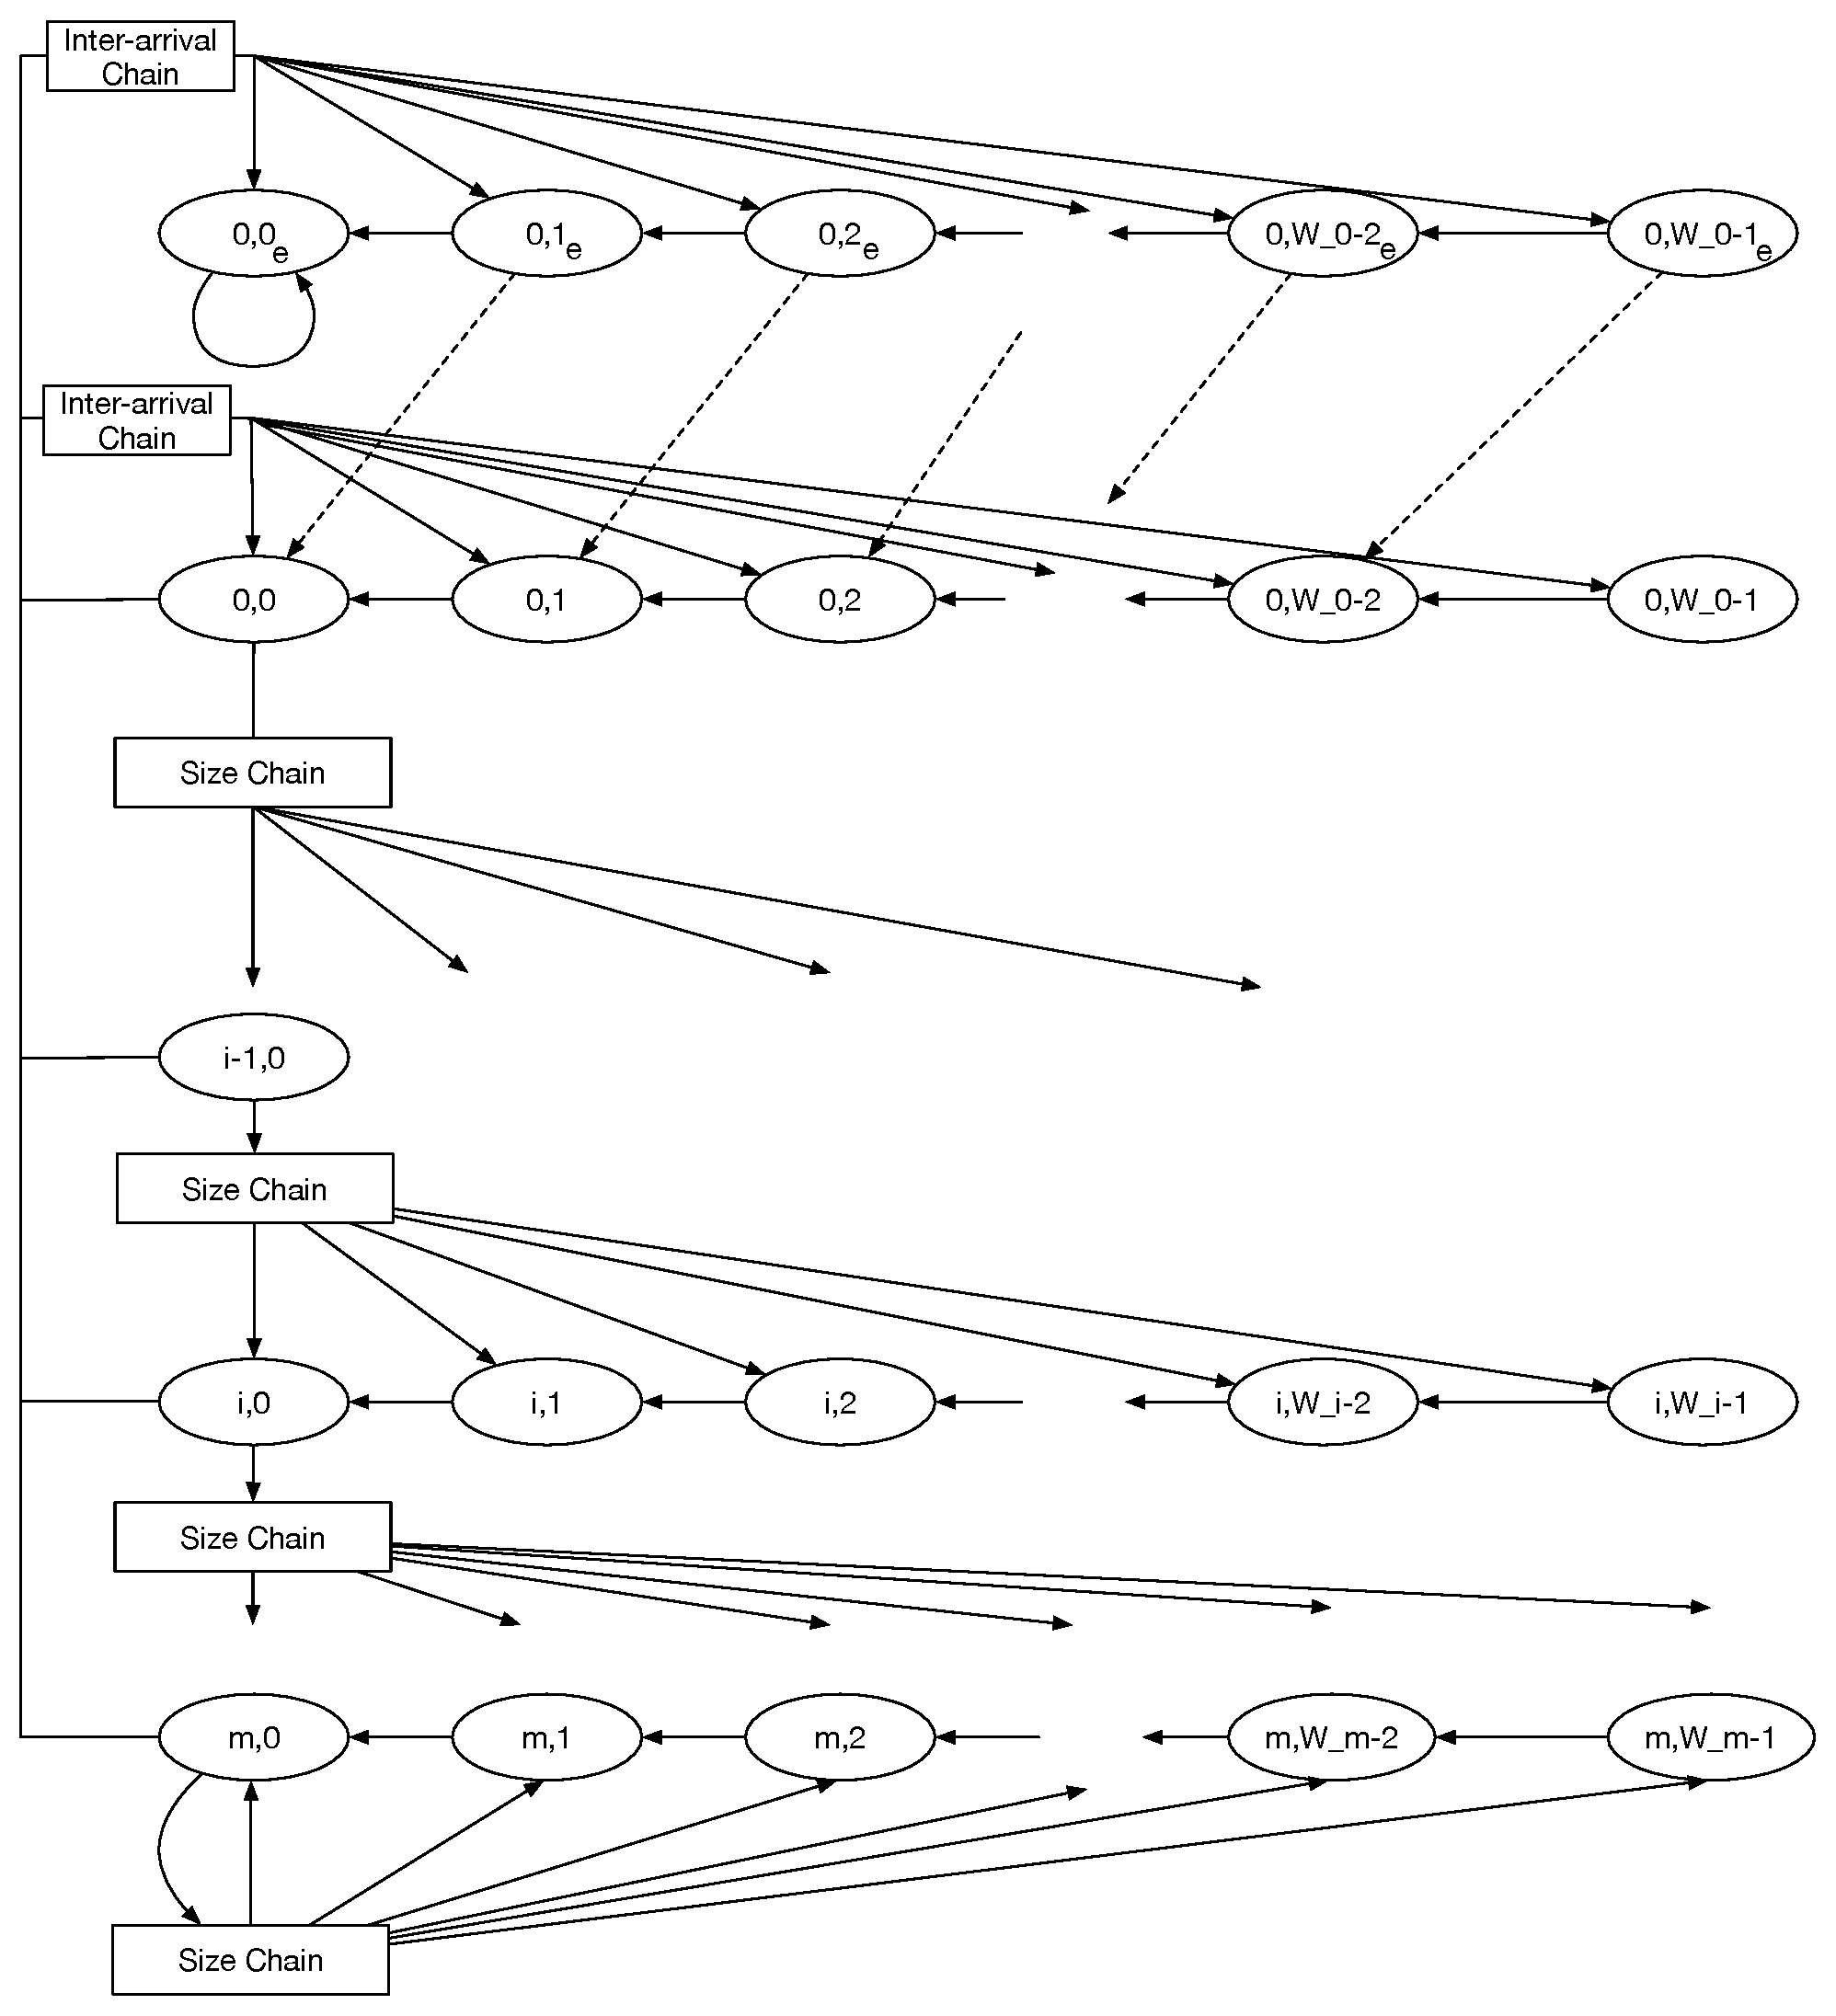
\includegraphics[scale=0.35]{../../sketches/dcf_model_unsaturated_varpktsize_interarrival.pdf}
\caption{The modified unsaturated DCF Markov model that captures variable-length packet payloads.}
\label{fig:dcf_model_unsaturated_varpktsize_interarrival}
\end{center}
\end{figure*}

\section{Simulator Design and Implementation}
A major part of this research was developing a simulator that could manage the growing complexity of the multi-dimensional Markov state. To this end, in this section we describe the relevant design and implementation details that were used to realize the analytical models just described. These details will be of importance to those seeking to extend our tunable analytical models. 

\subsection{Managing Markov Model Dimensional Complexity}
By adding more tunable parameters to Bianchi's 2-dimensional DCF, we needed a way to manage the growing complexity of the model. We accomplished in two ways:
\begin{enumerate}
	\item Creating small Markov models for each ``state'' of the system, i.e., the packet size calculation, treating them as black boxes.
	\item Use ``compressible'' states as logical and instantaneous bridges between Markov model black boxes.
\end{enumerate}
An example of a compressible state is shown in Figure \ref{fig:collapses}. Observe that the $x1$ and $x2$ states are the ``bridges'' between the states $S1$ and $S2,S3,S4$. When ``compressed'', the transition probabilities between $S1$ and $S2$, for example, becomes the product of the transition probabilities into and out of the compressible state. 

\begin{figure*}
\begin{center}
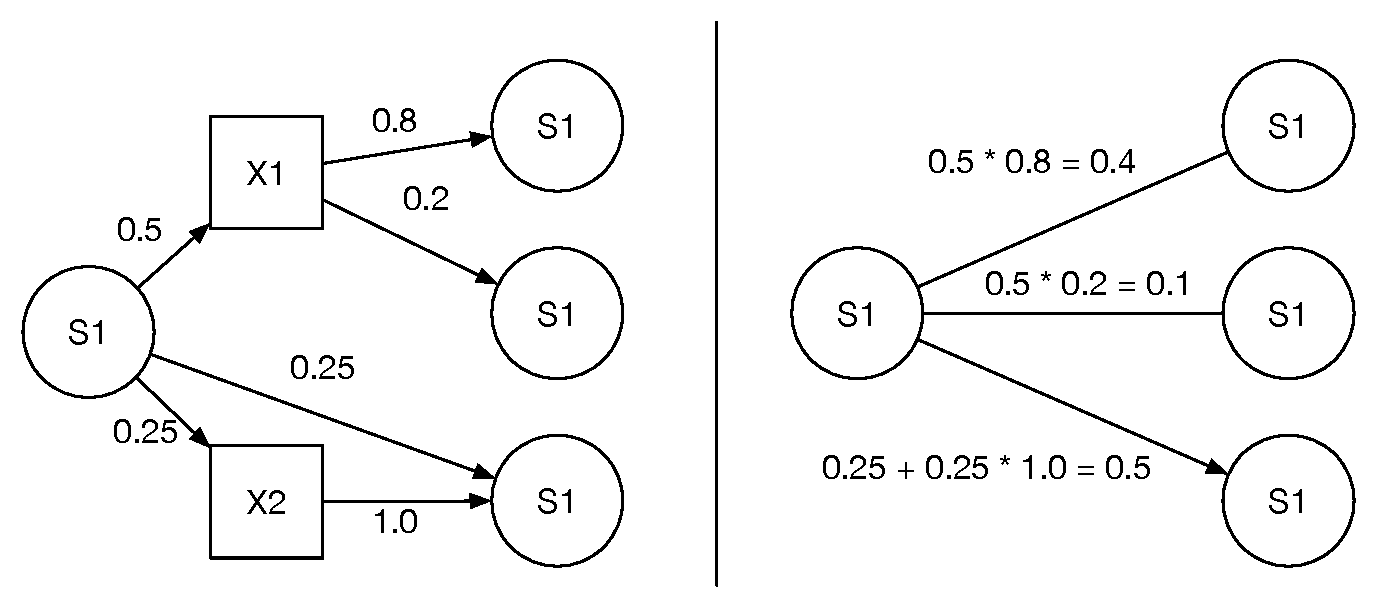
\includegraphics[scale=0.4]{../../sketches/collapses.pdf}
\caption{A sample usage of ``compressible'' states that bridge the transition gap between separate Markov chains.}
\label{fig:collapses}
\end{center}
\end{figure*}

To illustrate the efficacy of these states, consider the compressible variant of the DCF model shown in Figure \ref{fig:compressible_dcf}. It is easy to see its equivalence to the original DCF model after the compressible (green) states are compressed. Our implementation uses these compressible states to bridge between separate Markov chains. In this case, we treat each backoff timer stage as a separate chain. Moving between these chains, either through transmission success or failure, happens through compressible states.

\begin{figure*}
\begin{center}
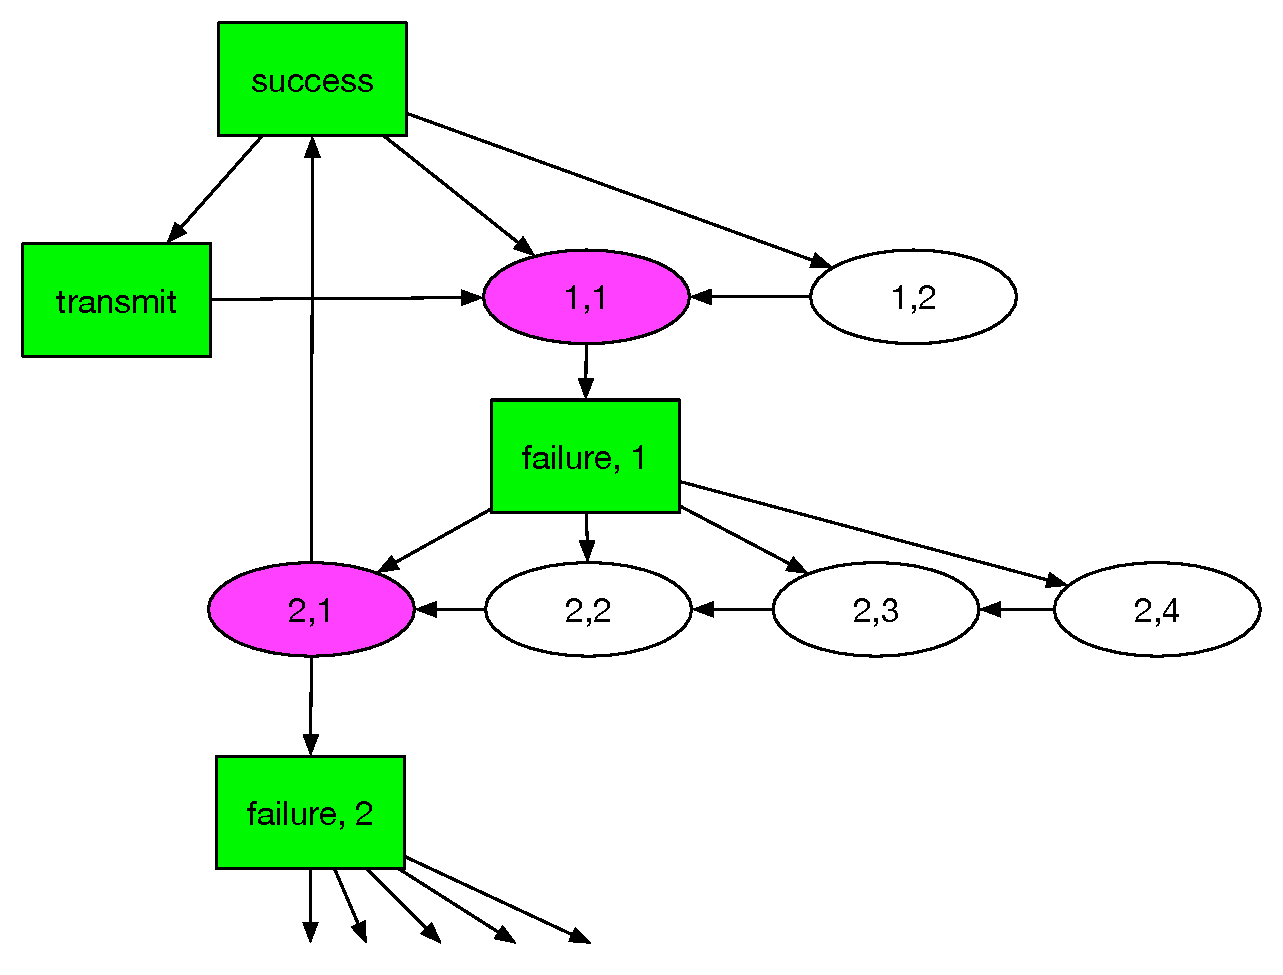
\includegraphics[scale=0.45]{../../sketches/compressible_dcf.pdf}
\caption{Bianchi's DCF model represented using compressible states. Green states are collapsible.}
\label{fig:compressible_dcf}
\end{center}
\end{figure*}

With this representation, adding support for the postbackoff, interarrival, and packetsize Markov chains is simple. To this end, consider the extended Markov model shown in Figure \ref{fig:compressible_dcf_arrival}. After a packet successfully transmits, it enters the {\sf transmit} state, indicating that it is ready to transfer another packet. If there is a non-zero probability of an interarrival time greater than one (1), the transmit state will enter the {\sf inter-arrival} state. Then, depending on the distribution of the interarrival times, the state will transition into the interarrival chain at the appropriate index. Notice that the index into this chain determines the interarrival time. 

As an example, let the interarrival time be a discrete random variable with uniform distribution sampled from the range [1,3]. If the interarrival time is determined to be 3, which will happen with probability exactly 1/3, then the chain will enter the index at state 3. Since the probabilities between the interarrival chain states are deterministic with probability 1.0, this means that there \emph{will always} be 3 epochs before the state transitions out of the interarrival chain and into the ``ready-to-transmit'' state. 

\begin{figure*}
\begin{center}
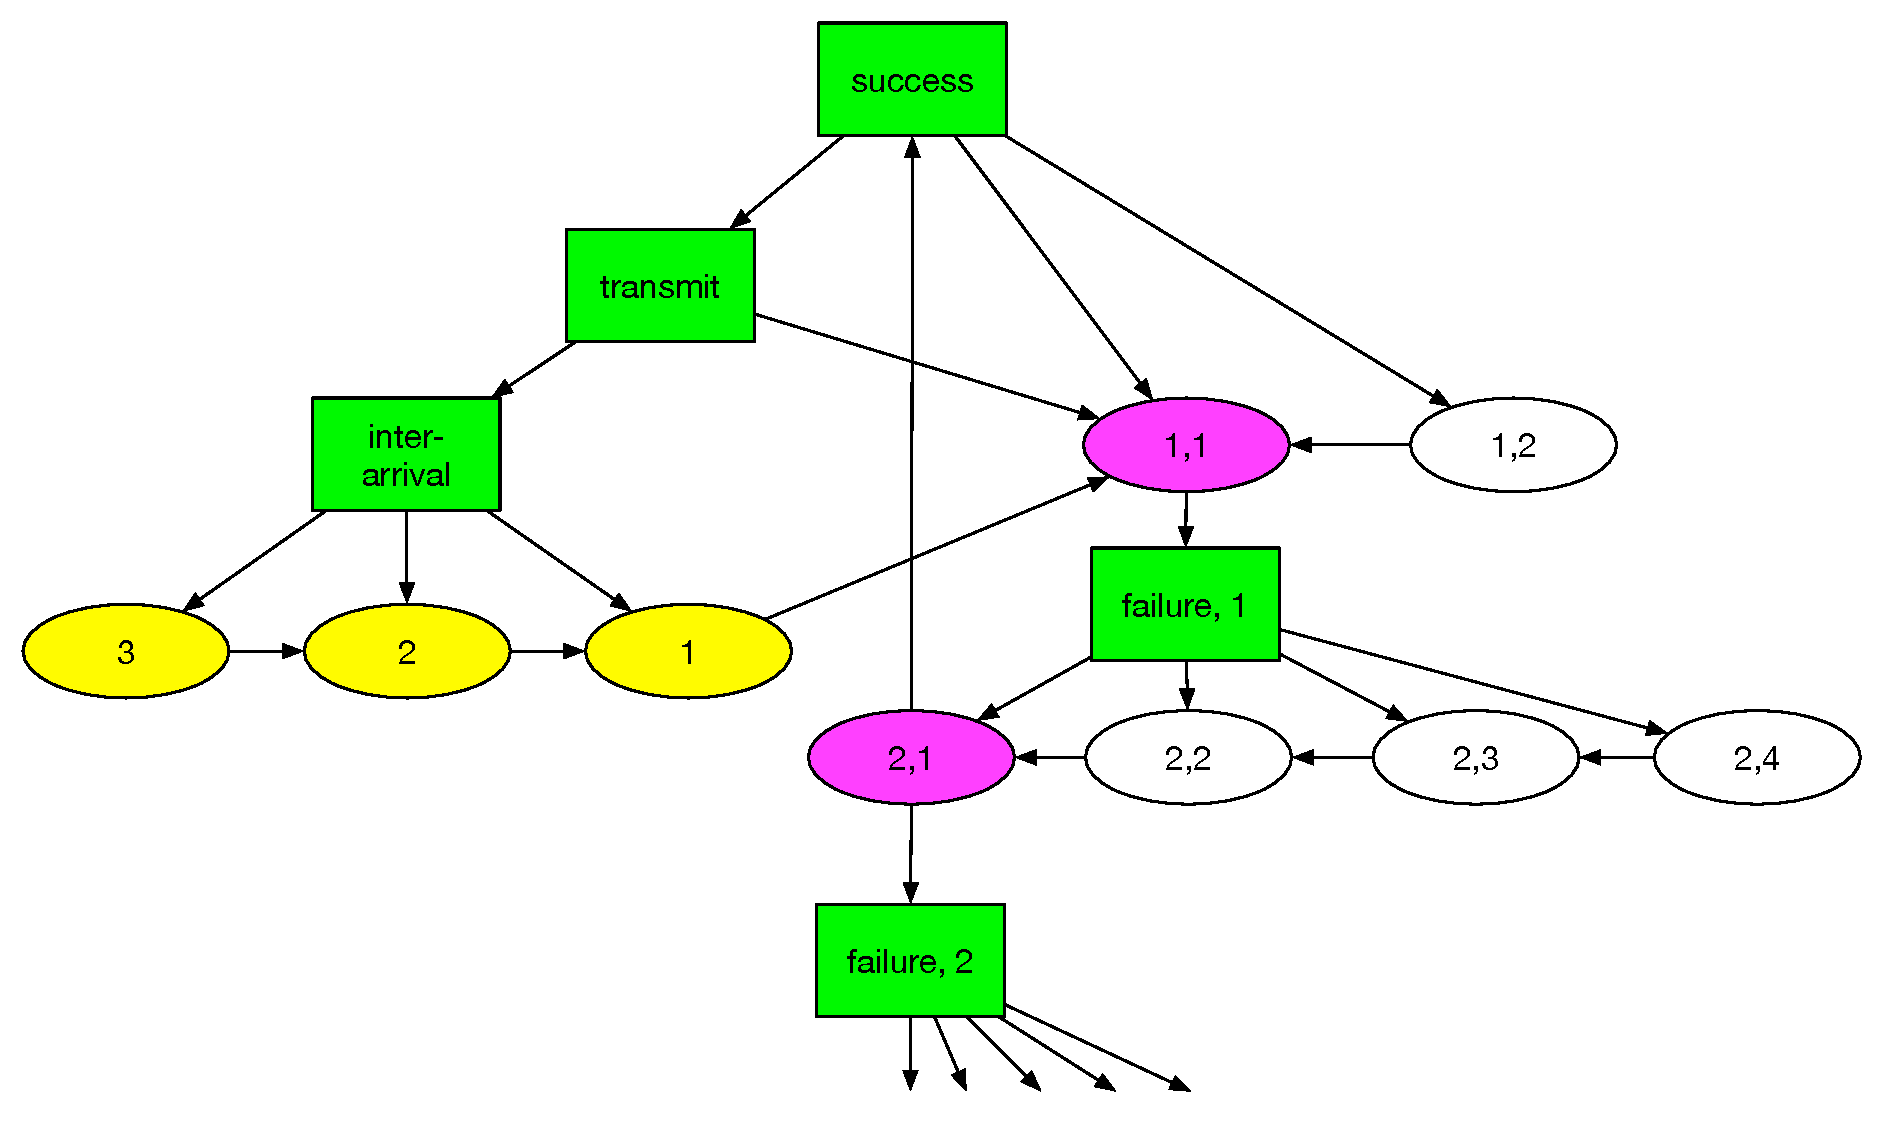
\includegraphics[scale=0.4]{../../sketches/compressible_dcf_arrival.pdf}
\caption{The extended compressible DCF model with support for parameterized interarrival times.}
\label{fig:compressible_dcf_arrival}
\end{center}
\end{figure*}

To support different packet lengths, we follow the approach outlined in the previous section and use packet size chains, which are similar to interarrival time chains, before attempting to transmit a packet. We emphasize here that the implementation does not strictly adhere to the model previously described. The astute reader will have observed that the model should compute the size of a packet \emph{once}, and then use that same packet size for every transmission attempt. The extension we presented in the previous section recomputes the packet size at every transmission attempt. We presented the model this way for clarity only. 

In the actual implementation, a packet size range of length $n$ is modeled by \emph{duplicating} the extended DCF model $n$ times, where each copy has $i = 1,\dots,n$ has a packet size chain of length $i$ at the ``beginning'' of the model. This is illustrated in Figure \ref{fig:compressible_dcf_all}, where, after a packet arrives, the state of the system transitions into the copy with the appropriate packet size chain. For example, let the packet size be a discrete random variable sampled from [1,3] with a uniform distribution. With probability 1/3 the state of the chain will transition into the the DCF copy (black box) with the packet size of length $1$, where it will remain until the packet is transmitted successfully. 

\begin{figure*}
\begin{center}
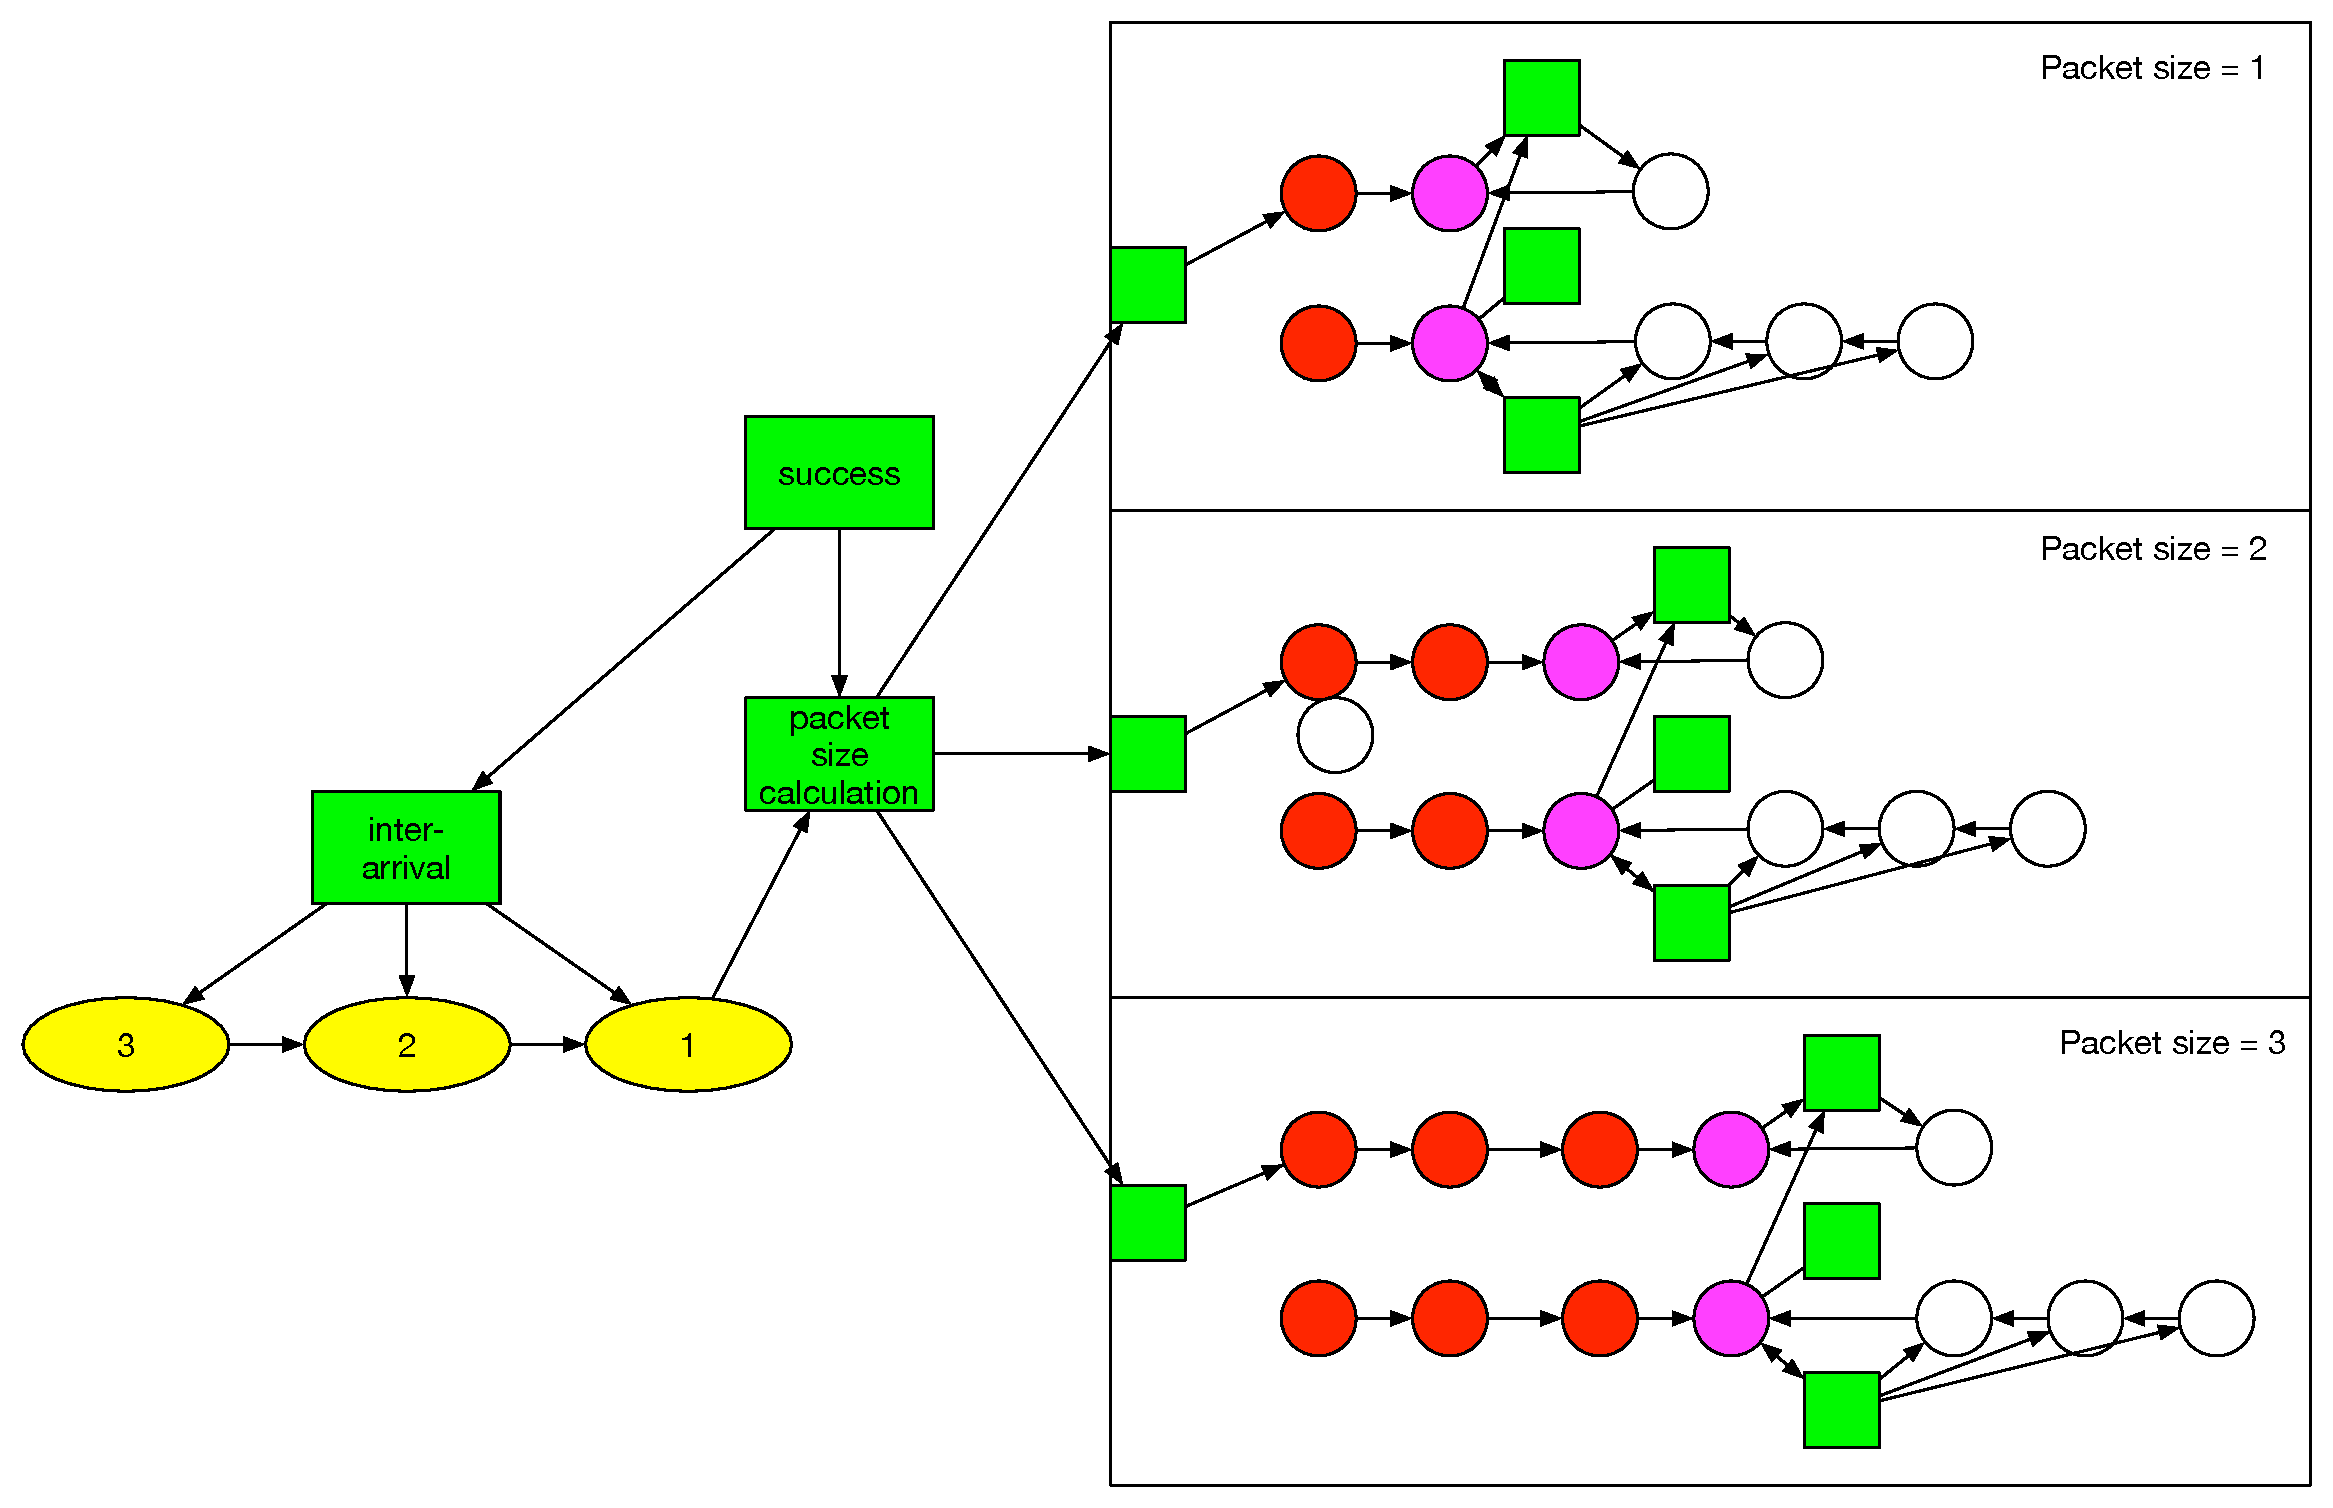
\includegraphics[scale=0.35]{../../sketches/compressible_dcf_all.pdf}
\caption{The extended compressible DCF model with support for parameterized packet lengths.}
\label{fig:compressible_dcf_all}
\end{center}
\end{figure*}

\subsection{Multi-Node Simulator Overview and Metrics Computations}

Having described the architecture of the Markov chain, we now describe how we implement the multi-node simulator using individual instances of these chains. Let $N$ be the number of nodes in a system, each with a unique set of traffic characteristics and, therefore, a unique Markov model, state space, and transition probability matrix. The simulator maintains a collection of individual simulator nodes, each one with its own Markov chain state space and probability transition matrix. At each time step, the simulator advances the state of each node according to the current system state and its individual state. For example, if at time $t$ the simulator sees that nodes $n_i$ and $n_j$ are trying to transmit, then the simulator will advance each from its current state by setting $p = 1.0$. Ultimately, the state of the collection of nodes determines network-based parameters such as $p$, the conditional collision probability. The simulator algorithm is shown in Figure \ref{alg:simulator}. 

\begin{figure*}
\begin{algorithmic}
\REQUIRE{$N$ simulator nodes $n_1,\dots,n_N$, and a time step limit $T$}
\FOR{$t = 1 \to T$}
	\STATE {Determine if there is a collision based on current node states}
	\FOR{$i = 1 \to N$}
		\STATE $p_i := 1.0$ if $n_i$ is in a collision, else $p_i = 0$
		\STATE{Advance the state of $n_i$ with $p_i$, and record the transition}
	\ENDFOR
\ENDFOR
\end{algorithmic}
\caption{The multi-node simulator algorithm.}
\label{alg:simulator}
\end{figure*}

The master simulator individual simulator nodes are also responsible for bookkeeping relevant events. Specifically, traces of state transitions are recorded so that the entire system dynamics can be replayed and relevant metrics can be computed about both individual nodes and the group as a whole. In our work, we mainly consider the following metrics: throughput, packet transmission success probability, and packet failure probability. Let $n$ be the total number of steps in the simulation, $s$ be the number of successful transmissions, and $f$ be the number of failed transmissions. Throughput $S$ is defined as the ratio of successful transmissions out of \emph{all} possible time steps in the system, i.e., $S = p / n$. The success probability $P_s$ is defined as the number of success transitions compared to the number of transmission attempt transitions, i.e., $P_s = p / (p + f)$. Finally, the packet failure probability $P_f$ is defined as the number of failied transitions compared to the number of transmission attempts, i.e., $P_f = f / (p + f)$. 

\section{Experimental Setup} \label{sec:experiment}
To test our experiment, we ran the simulation on the system and traffic configurations listed in Tables \ref{tab:configurations}, \ref{tab:traffics}, and \ref{tab:multimedia}. Traffic parameters with ranges of values are sampled according to the distribution specific that that type of traffic. For example, file download packet sizes are sampled uniformly from the given packet range. 

Notice that we limited our study to small backoffs and only two nodes. The reason for this restriction was two-fold. Firstly, having more than one node increased the number of variables in our experiments. In order to accurately assess the influence of any \emph{single} variable on the individual node and overall system performance. Consider Figures \ref{fig:smallwindow} and \ref{fig:multinodes}. In the former, we see that the throughput metric variance is much more distinct with small backoff windows (i.e., the slope of the throughput change is steeper). In the latter, it is unclear what factors are influencing the throughput since there are so many variables. We could consider all parameter combinations in the multiple node setting, but with at least four parameters in each node with at least five values for each parameter, such an analysis would be intractible. Thus, we limit ourselves to multinode settings with $N = 2$ to simplify our analysis. 

We comment that since we do not study the time to conduct each experiment, the actual simulation machine parameters are not important. These details are omitted for space. 

\begin{table}
\begin{center}
\caption{System configuration parameters.}
\label{tab:configurations}
\begin{tabular}{|c|c|} \hline
	Time Steps & 100000 \\
	$W_{min}$ & 2 \\
	$W_{max}$ & 16 \\
	$m$ & 4 \\ \hline
\end{tabular}
\end{center}
\end{table}

\begin{table}
\begin{center}
\caption{Application traffic configuration parameters.}
\label{tab:traffics}
\begin{tabular}{|c|c|c|c|c|} \hline
	Traffic Type & \multicolumn{4}{c|}{Parameter Values} \\ \hline
	~ & Interarrival Time & Packet Size & P(Arrive) & P(Interarrival) \\ \hline \hline
	Random & \{0,1,2,3,4,5\} & \{1,2,3,4,5\} & \{0.0, 0.25, 0.5, 0.75, 1.0\} & \{0.0, 1.0\} \\ \hline
	Web Browsing & \{5\} & \{1\} & \{1.0\} & \{0.5, 0.6, 0.7, 0.8, 0.9, 1.0\} \\ \hline
	File Download & \{5, 10, 25\} & \{5, 10, 25\} & \{1.0\} & \{1.0\} \\ \hline
\end{tabular}
\end{center}
\end{table}

\begin{table}
\begin{center}
\caption{Multimedia traffic configuration parameters.}
\label{tab:multimedia}
\begin{tabular}{|c|c|} \hline
	Parameter & Values \\ \hline
	BPS & \{2MB/s, 4MB/s, 8MB/s, 16MB/s, 32MB/s\} \\
	Payload Size & \{12000b\} \\ \hline
\end{tabular}
\end{center}
\end{table}

\begin{figure*}
\begin{center}
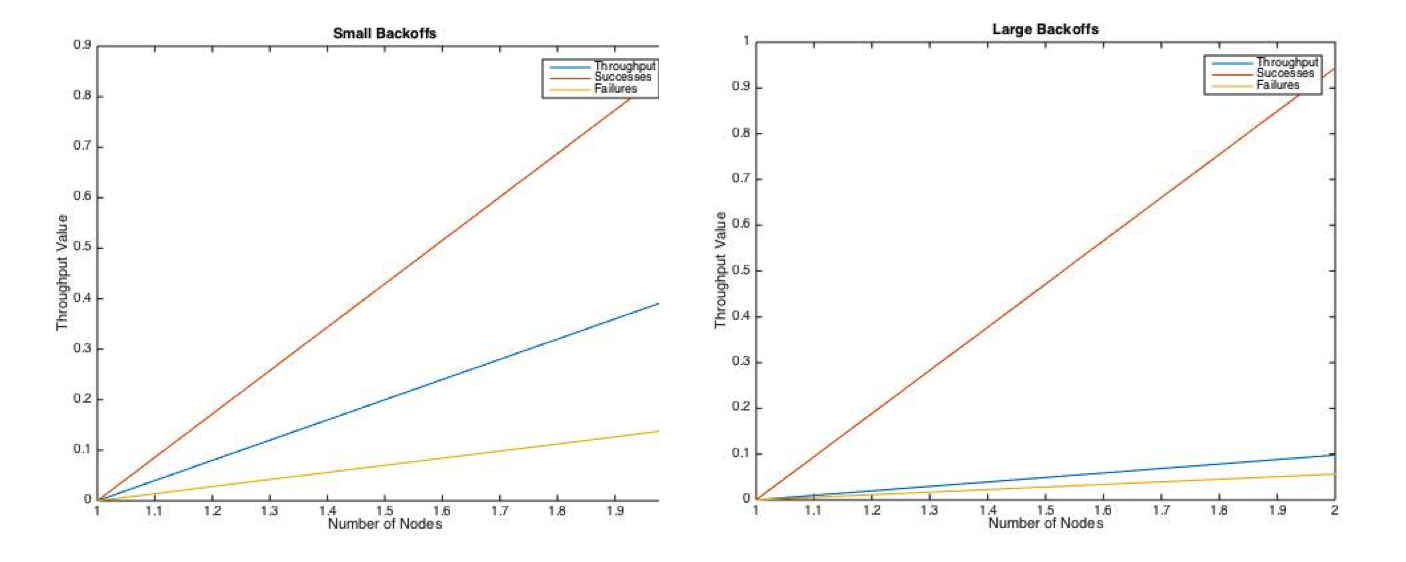
\includegraphics[scale=0.6]{smallwindow.png}
\caption{A comparison of the effect of a small backoff vs large backoff window. The small backoff window leads to much more pronounced changes in the metrics of interest, which lends itself to this analytical study.}
\label{fig:smallwindow}
\end{center}
\end{figure*}

\begin{figure*}
\begin{center}
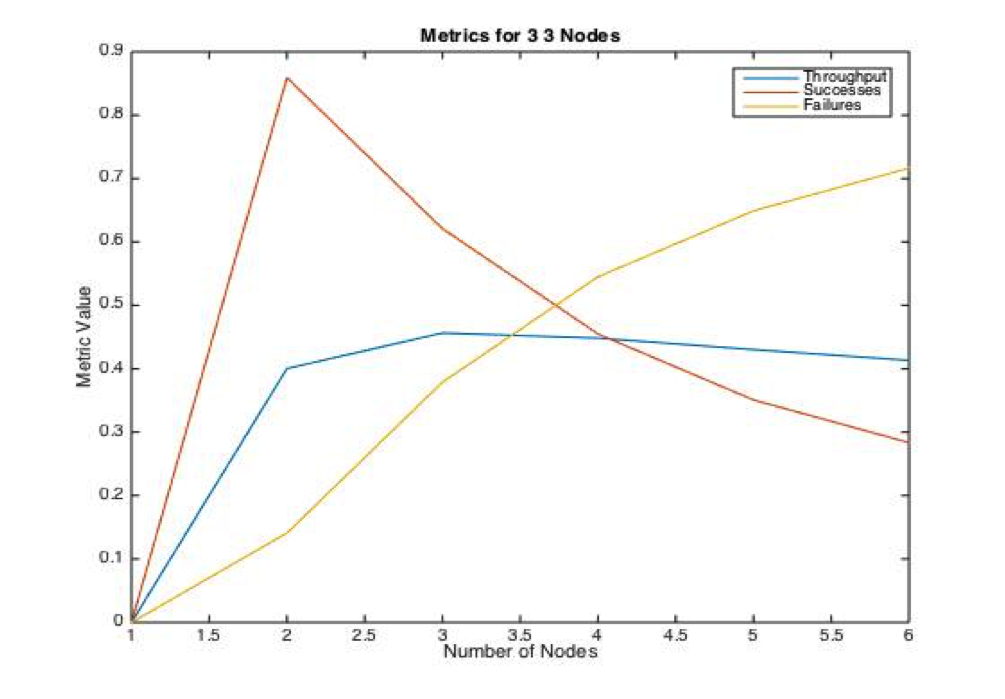
\includegraphics[scale=0.6]{multinodes.png}
\caption{Metric values as a function of the number of nodes added to the system.}
\label{fig:multinodes}
\end{center}
\end{figure*}

\section{Simulation Results and Analysis}
In this section we discuss the results of our simulations collected from the experimental setup prescribed in the previous section. We restrict our discussion to results that are noteworthy and only focus on throughput metrics\footnote{All other simulation parameter combinations were performed, and both packet success and failure probabilities are included as well. This data is provided in addition to this report. However, the analysis is omitted here due to lack of noteworthy results.} A subset of these cases is assessed below.

\begin{enumerate}
	\item Case 1 -- random node vs. multimedia node: In this case we study the coexistence of a random node and a multimedia node. The results are shown in Figure \ref{fig:randomstuff1}. In the left figure we see that the random node throughput remains constant -- approximately 0.68 -- even as the multimedia node streaming bitrate increases. In addition, the multimedia node throughput increases logarithmically towards an asymptote of approximately 0.4. This seems to imply that the random node traffic transmissions weave together with the multimedia transmission attempts. Since the packet lengths are small (1), they do not result in collisions, which is why neither throughput values decrease as the bitrate increases.

	In the right figure we see somewhat different behavior. Specifically, the random node throughput decreases to 0 as the bitrate increases. Conversely, however, the multimedia node throughput increases to the same asymptotic value as the previous case. This is indicative of more collisions that occur as a result of the larger packet lengths in the random traffic. Since the multimedia traffic generation pattern is deterministic, rather than random like its partner node, the multimedia node tends to get access to the channel before the random node. 

	\item Case 2 -- random node vs. file download node: In this case we study the coexistence of a random node and a file download node. The results are shown in Figure \ref{fig:randomstuff2}. We study the effect of both interarrival length and packet size length. In both cases, packet generation sources are random. However, both results seem to indicate that the random node throughput benefits at the expense of the download throughput. Specifically, the file download throughput remains at 0, whereas the throughput of the random node increases as both file download packet size and interarrival time increases. 

	With regards to interarrival time, we note that increased interarrival time means that the time between packet transmissions is also increased. Therefore, the random node successfully accesses the channel more frequently than the file download. Furthermore, when the file download does attempt to transmit, it collides with the random node, leading to continual failure. The same holds for the increased file download packet sizes. Longer packet sizes lead to an increased probability of collision for both nodes. However, the random node attempts to transmit more frequently since its packets are of shorter size, causing its throughput to not suffer.

	\item Case 3 -- random node vs. web browsing node: In this case we study the coexistence of a random node and a web browsing node. The results are shown in Figure \ref{fig:randomstuff3}. We study the effect of the interarrival probability for the web browsing node. A higher interarrival probability is indicative of traffic that is generally more sparse; if the probability is high then the node waits between packets with high probability. 

	In the left figure we see that, as the probability increases, the throughput for the random node remains constant -- approximately 0.68 -- and the web browsing throughput decreases from approximately 0.33 to 0.21. The cause of this is clear: as the interarrival probability increases, the number of packets that are generated for transmission decreases. Therefore, the throughput naturally decreases as well. We see similar results in the right figure, in which the random node has larger packet sizes. Observe that the random throughput is not constant. In fact, it oscillates around 0.2, whereas the web browsing throughput decreases just as in the previous case. We attribute this oscillating behavior to the fact that larger packet sizes, coupled with varying interarrival times by the competing node, lead to oscillating collision probabilities. Conversely,the throughput of the web browsing traffic decreases for the same reason as before: larger and more frequent interarrival times simply mean that less packets are transmitted.
\end{enumerate}

Based on these results, we make the following conclusions. First, the deterministic nature of multimedia (e.g., store-and-forward) traffic streams leads to higher performance (i.e., higher throughput) than more nondeteministic (elastic) traffic. Second, increasing interarrival times and packet sizes lead to (a) less chances to transmit packets and (b) higher probabilities of collision (this is not a new result). Lastly, less frequent non-zero interarrival times between packets benefit the performance of traffic, since it provides more opportunities for transmission.

%%% first
\begin{figure*}
\begin{tabular}{cc}
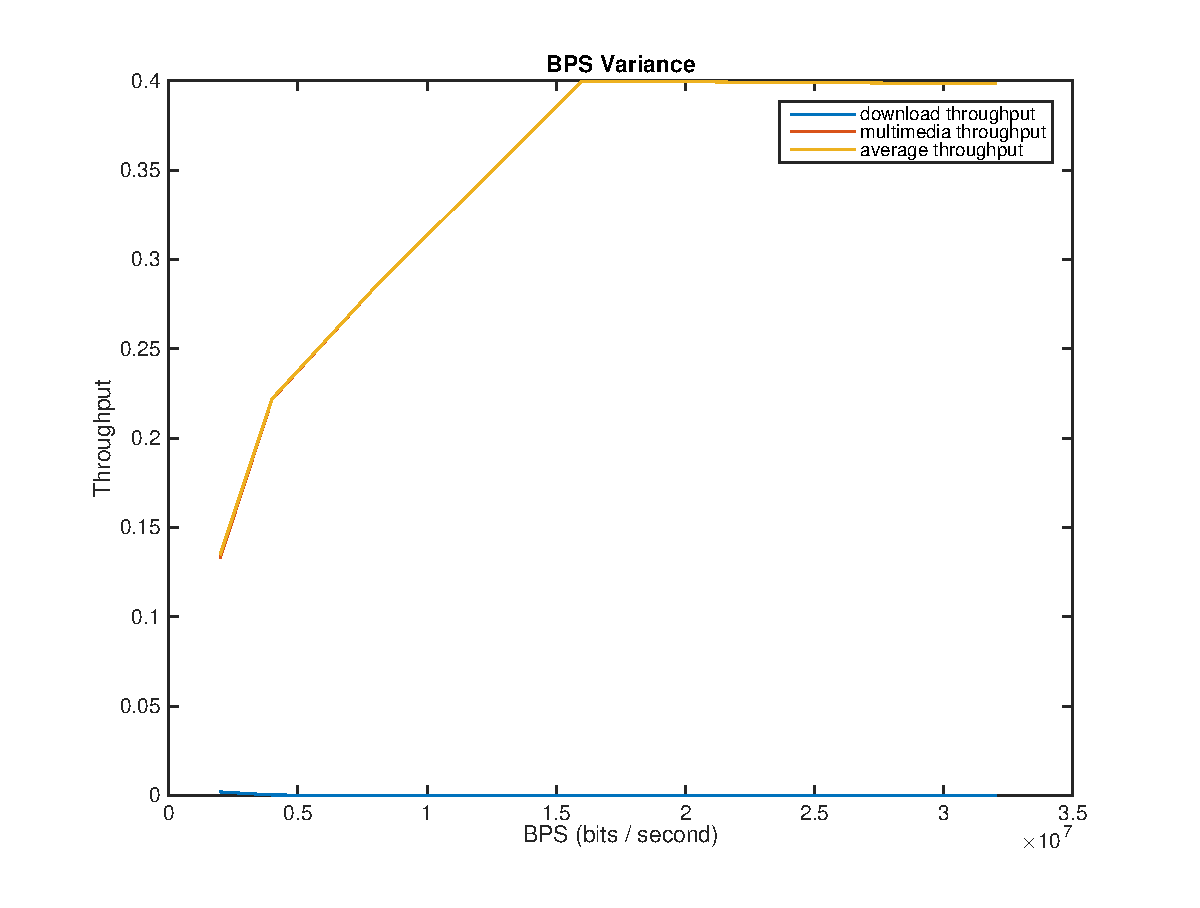
\includegraphics[scale=0.35]{../../src/fig-simulation_download_multimedia-bps-1_1_10_10_12000.eps} & 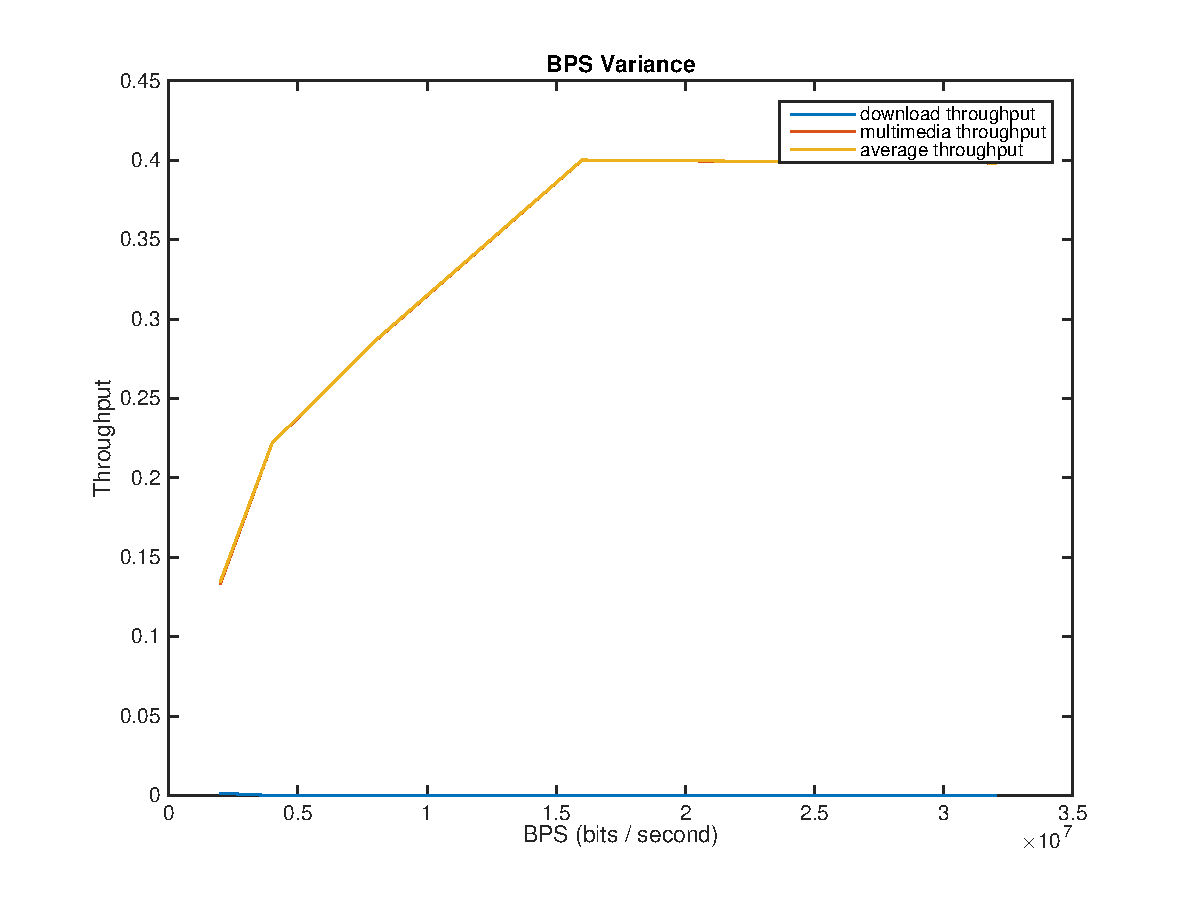
\includegraphics[scale=0.35]{../../src/fig-simulation_download_multimedia-bps-1_1_10_25_12000.eps} \\ 

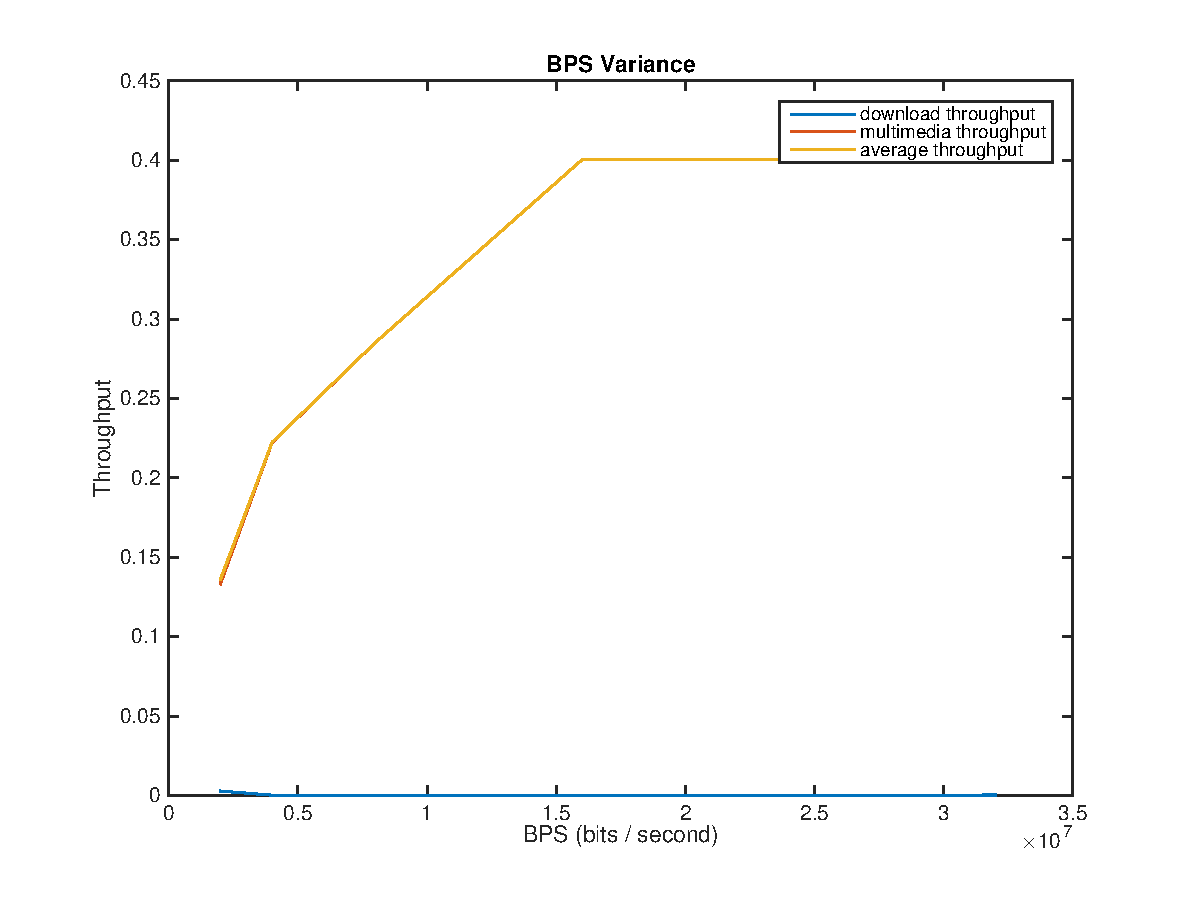
\includegraphics[scale=0.35]{../../src/fig-simulation_download_multimedia-bps-1_1_10_5_12000.eps} & 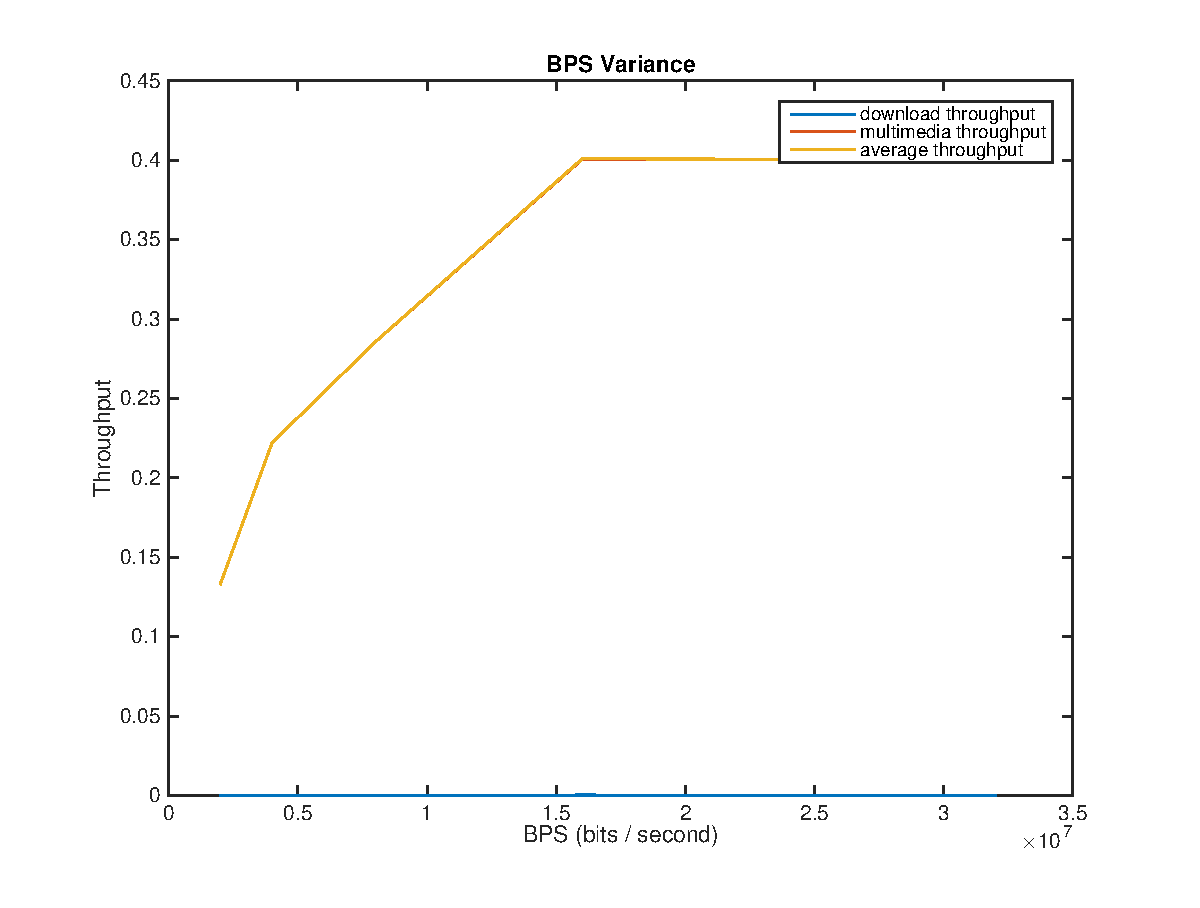
\includegraphics[scale=0.35]{../../src/fig-simulation_download_multimedia-bps-1_1_25_10_12000.eps} \\

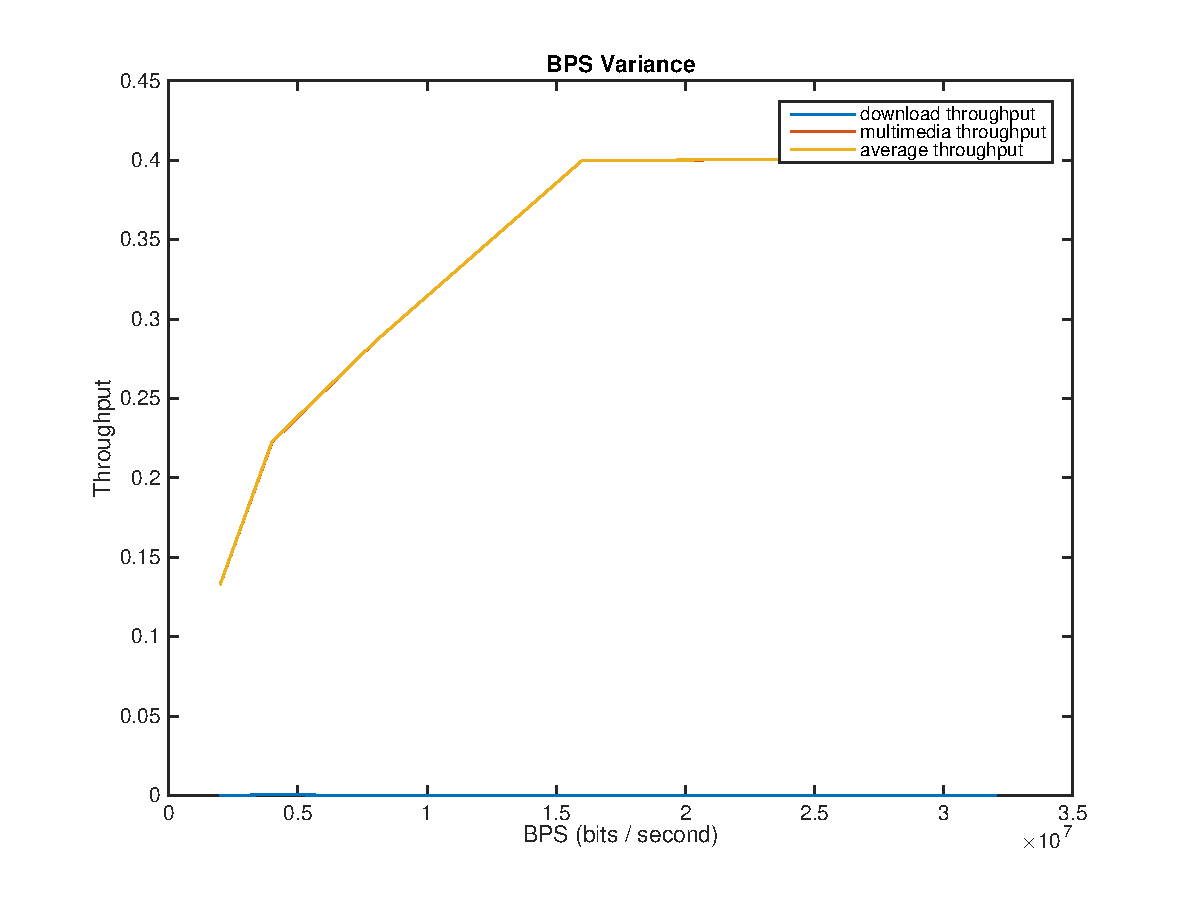
\includegraphics[scale=0.35]{../../src/fig-simulation_download_multimedia-bps-1_1_25_25_12000.eps} & 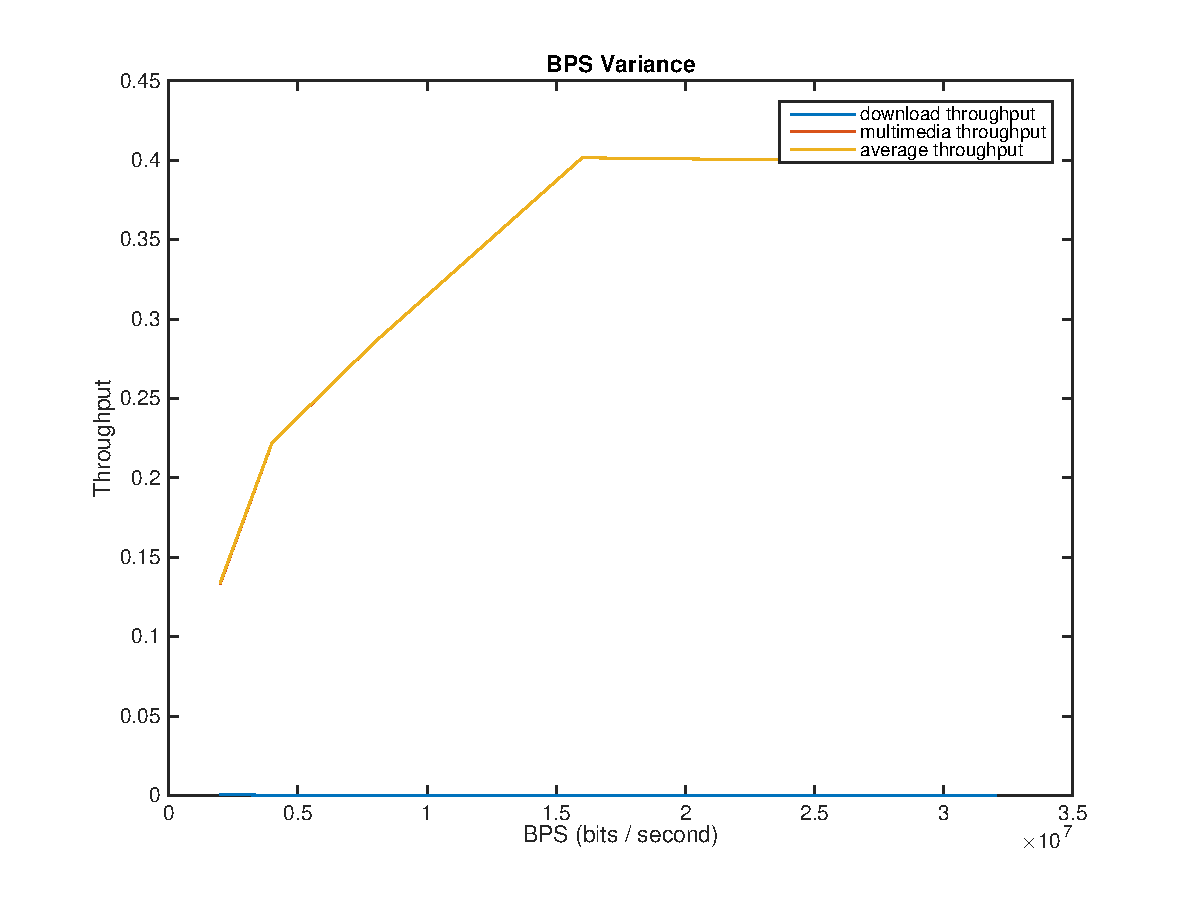
\includegraphics[scale=0.35]{../../src/fig-simulation_download_multimedia-bps-1_1_25_5_12000.eps} \\ 

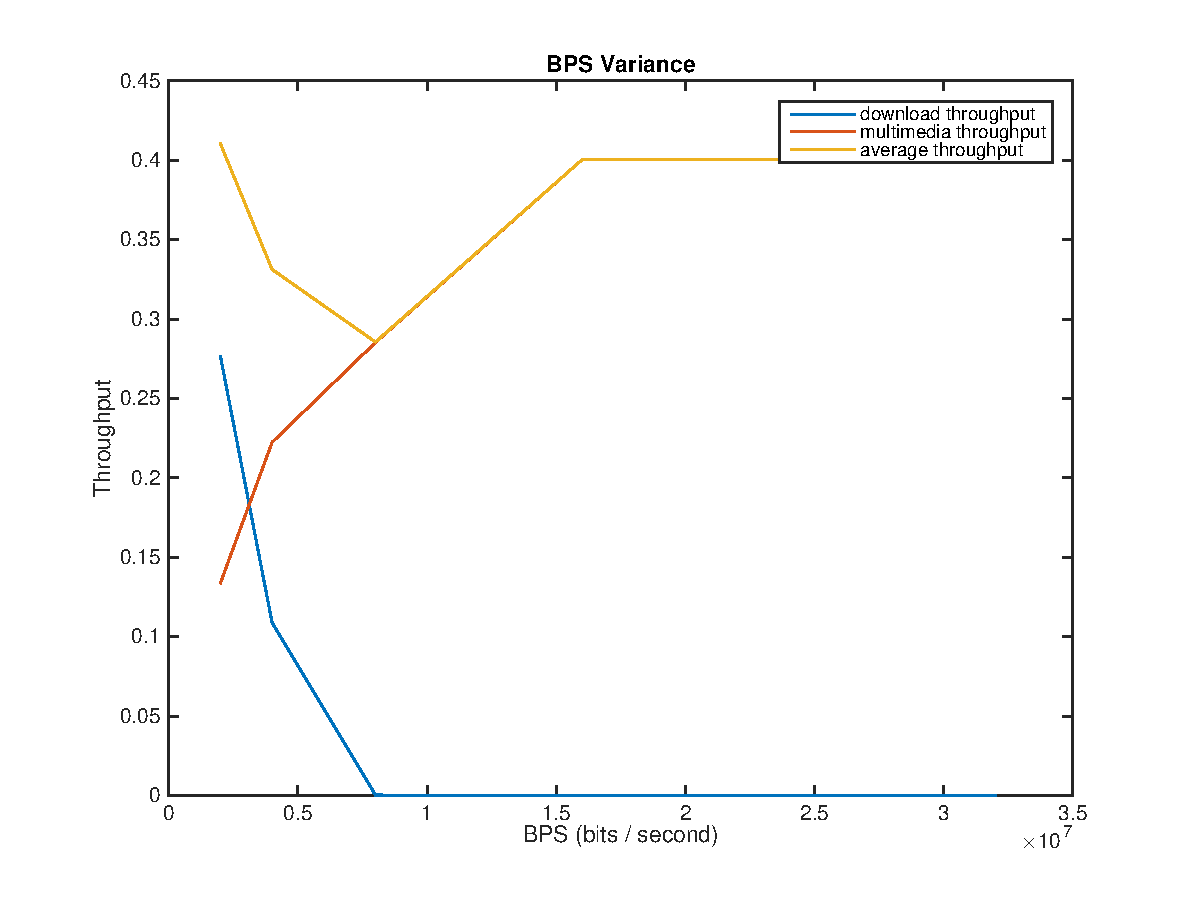
\includegraphics[scale=0.35]{../../src/fig-simulation_download_multimedia-bps-1_1_5_10_12000.eps} & 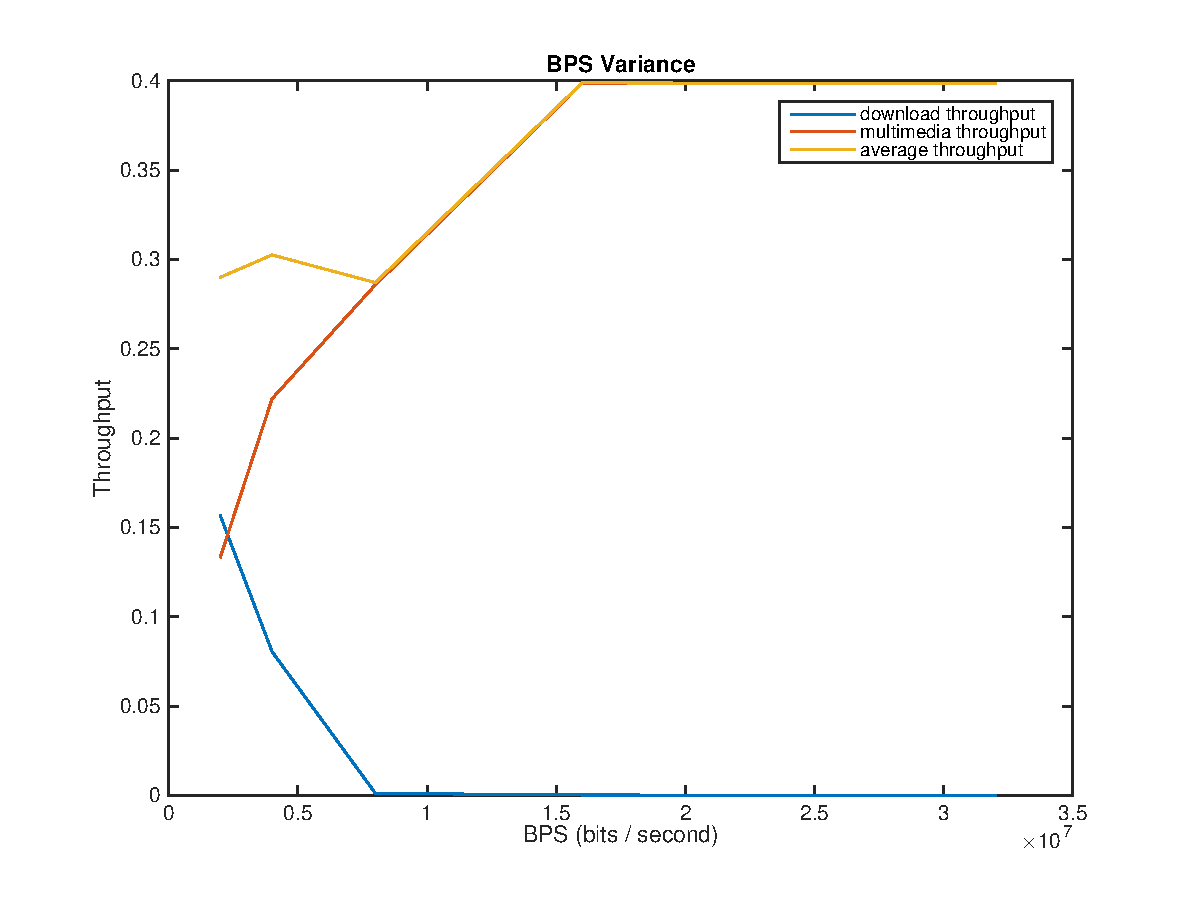
\includegraphics[scale=0.35]{../../src/fig-simulation_download_multimedia-bps-1_1_5_25_12000.eps}

\end{tabular}
\end{figure*}

%%% second
\begin{figure*}
\begin{tabular}{cc}

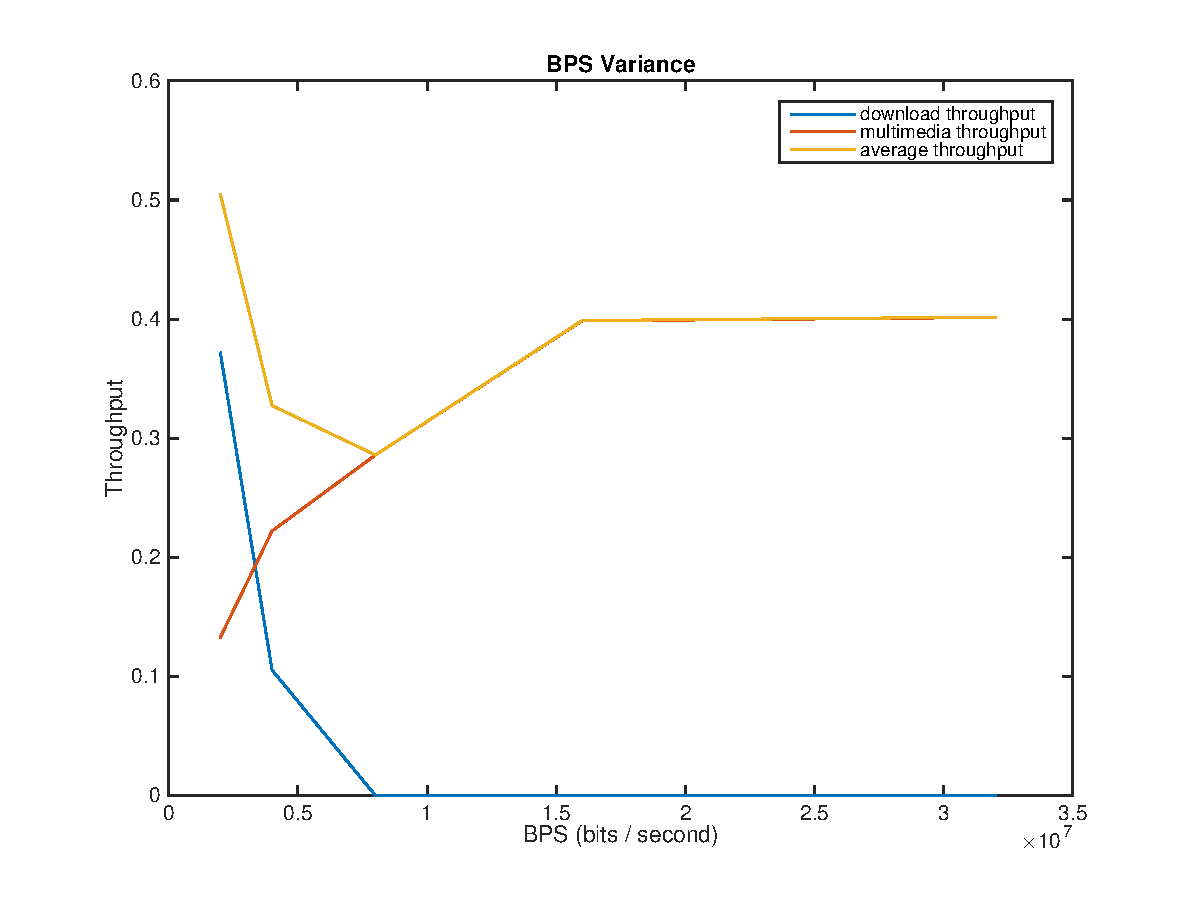
\includegraphics[scale=0.35]{../../src/fig-simulation_download_multimedia-bps-1_1_5_5_12000.eps} & 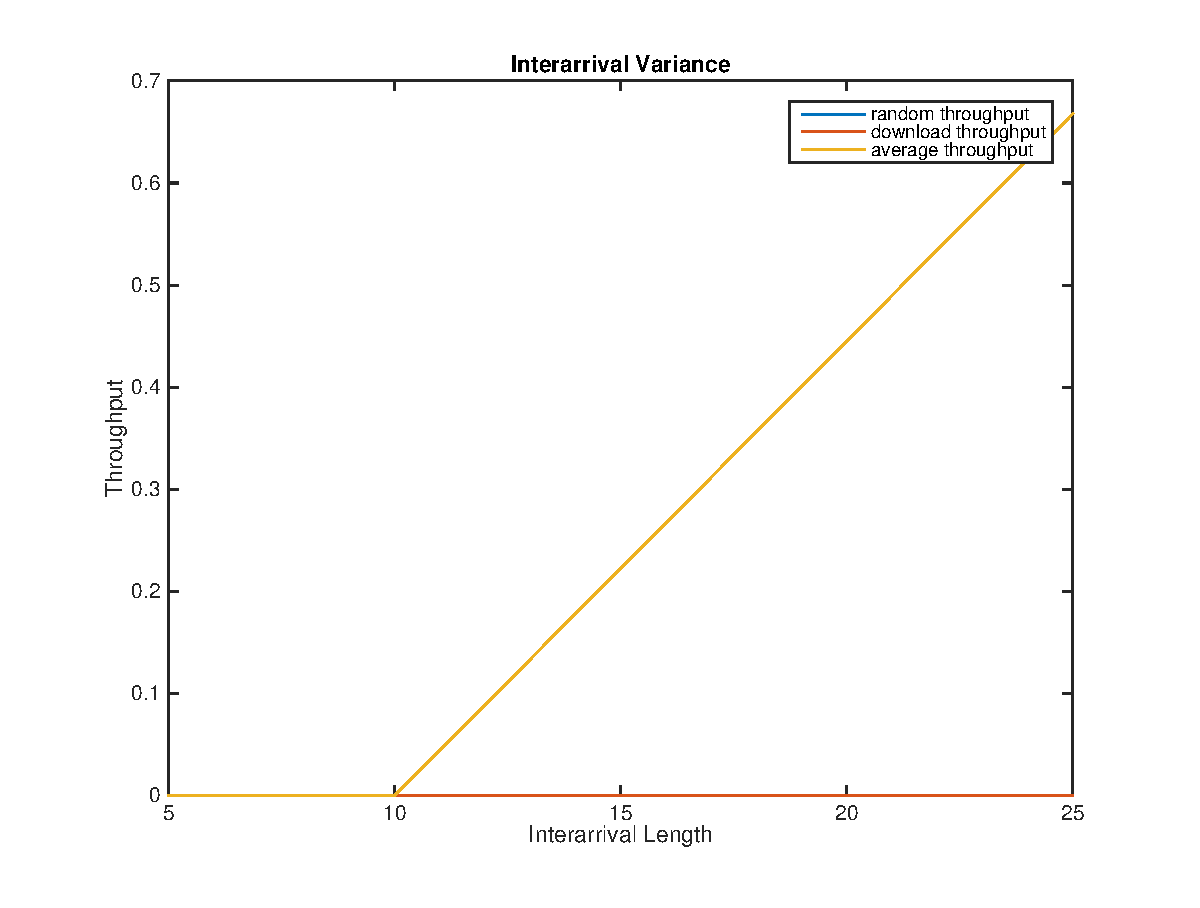
\includegraphics[scale=0.35]{../../src/fig-simulation_random_download-interarival-1_0_1_0_1_1_25.eps} \\
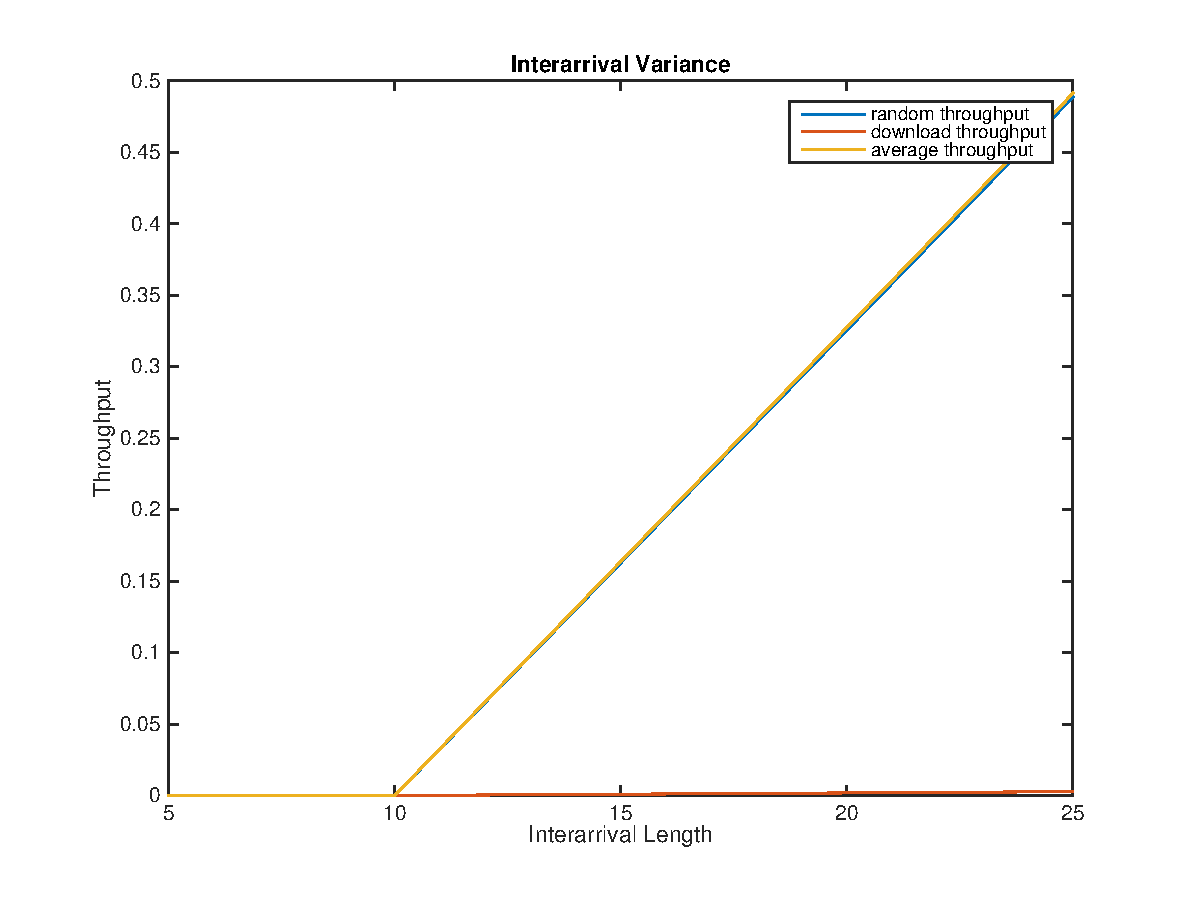
\includegraphics[scale=0.35]{../../src/fig-simulation_random_download-interarival-1_0_5_0_1_1_25.eps} & 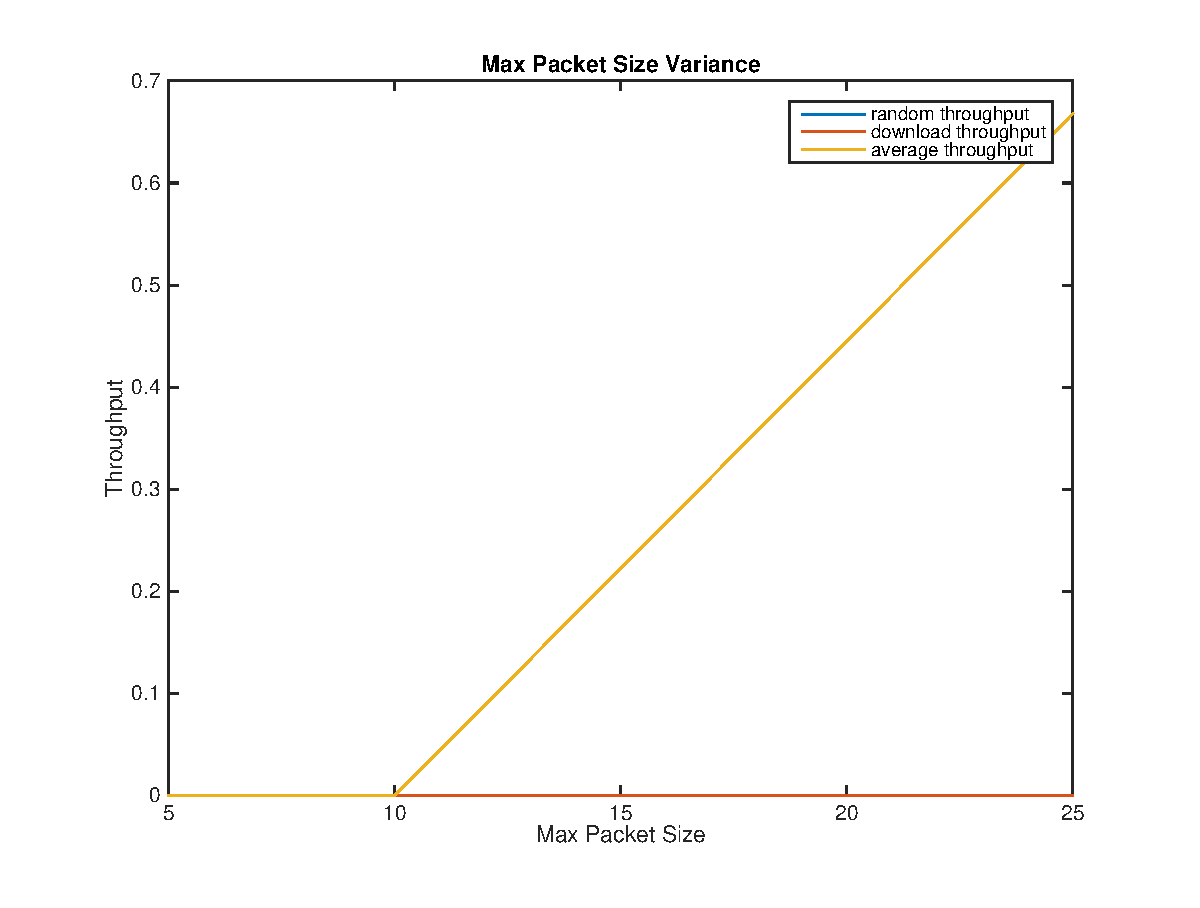
\includegraphics[scale=0.35]{../../src/fig-simulation_random_download-maxpackets-1_0_1_0_1_1_25.eps} \\
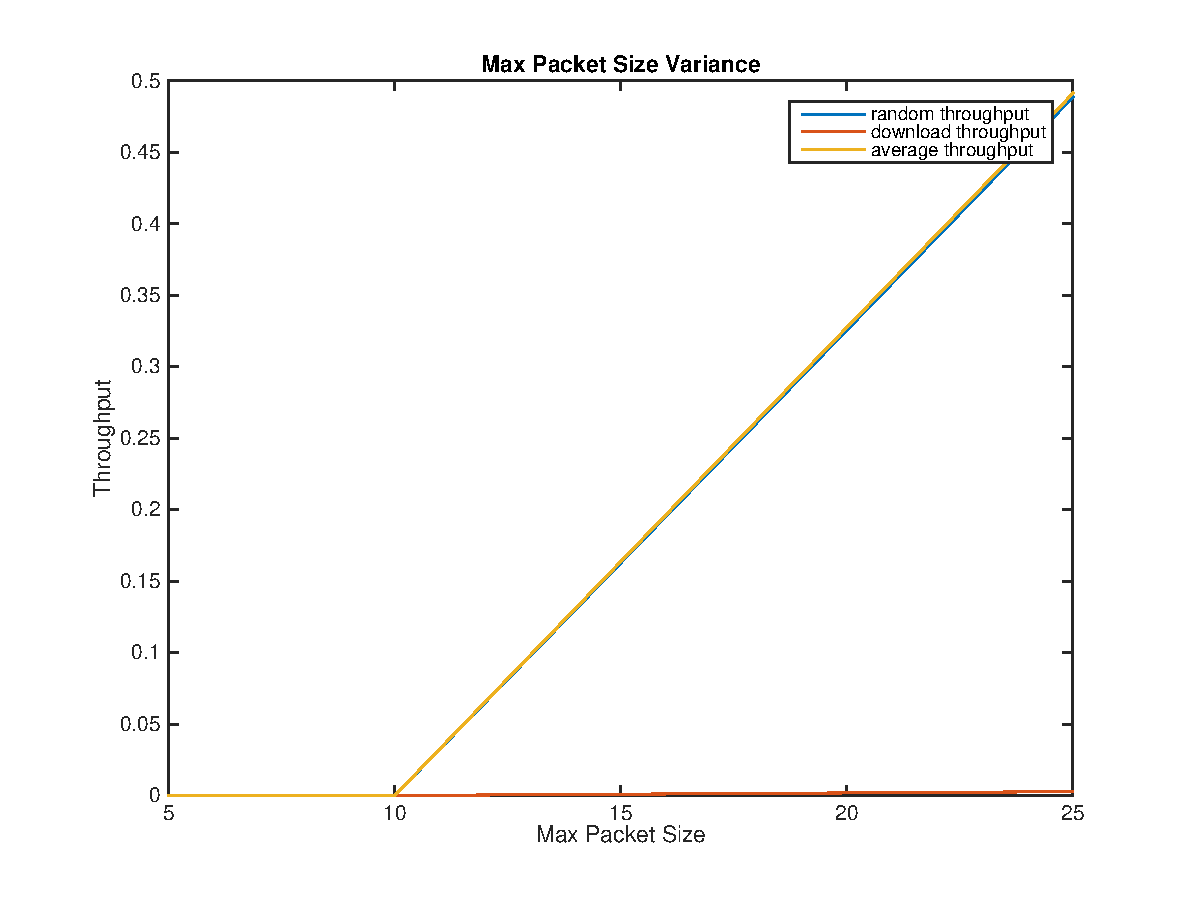
\includegraphics[scale=0.35]{../../src/fig-simulation_random_download-maxpackets-1_0_5_0_1_1_25.eps} & 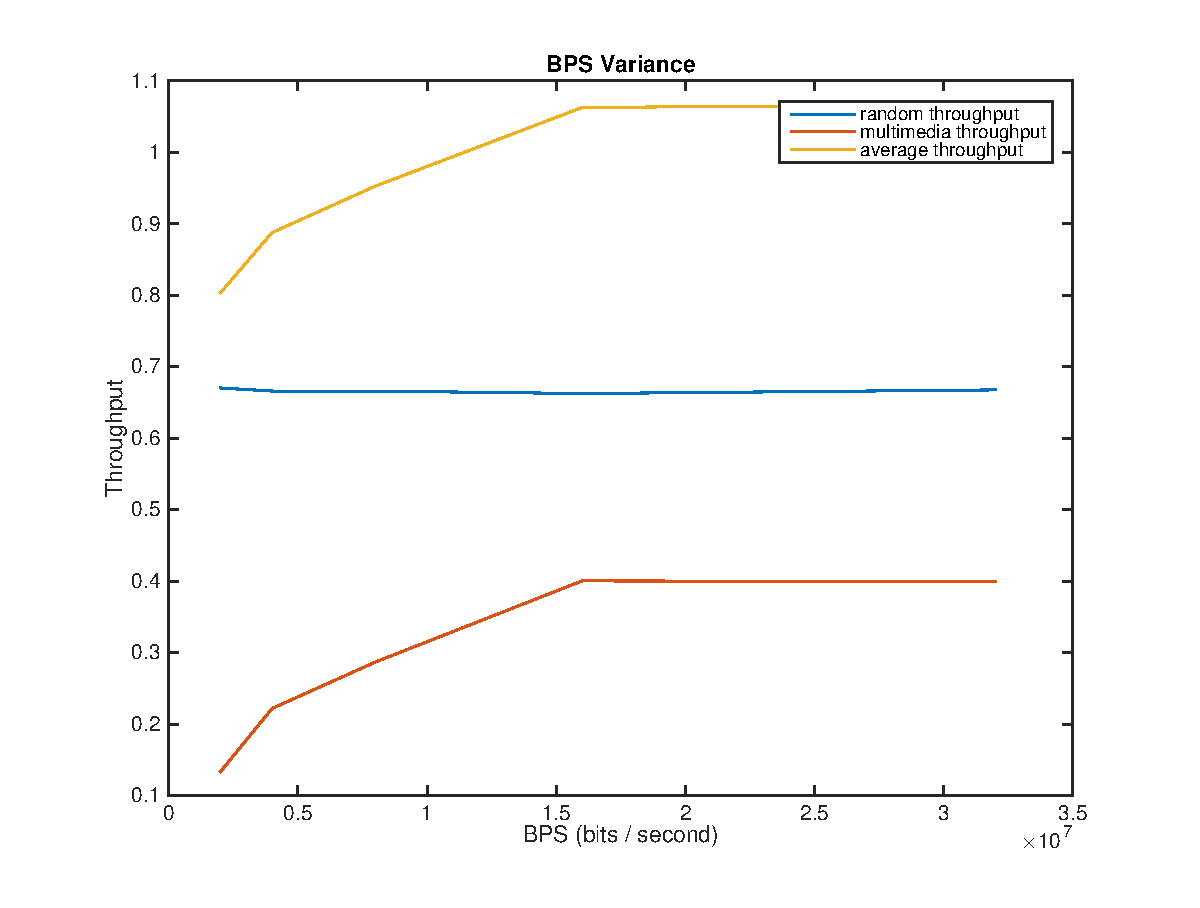
\includegraphics[scale=0.35]{../../src/fig-simulation_random_multimedia-bps-1_0_1_0_12000.eps} \\
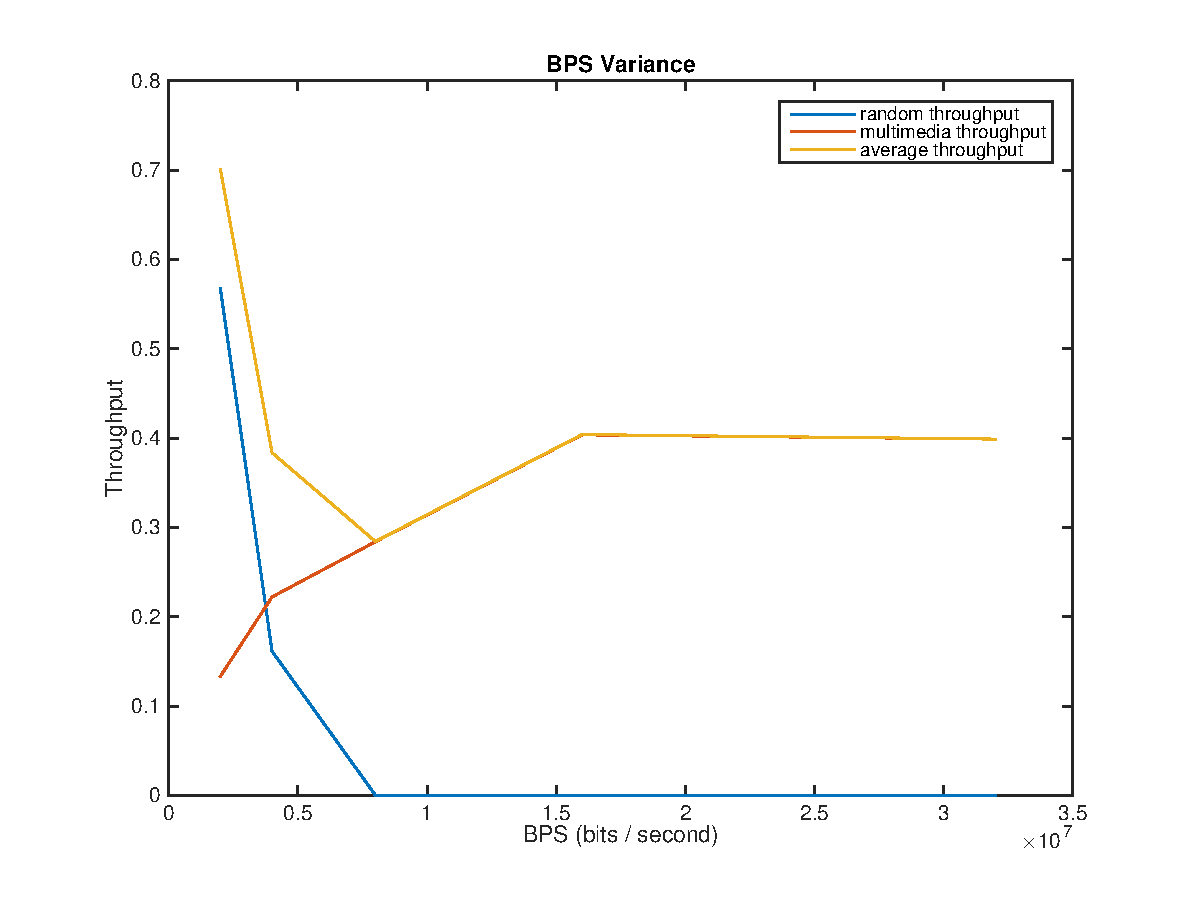
\includegraphics[scale=0.35]{../../src/fig-simulation_random_multimedia-bps-1_0_5_0_12000.eps} & 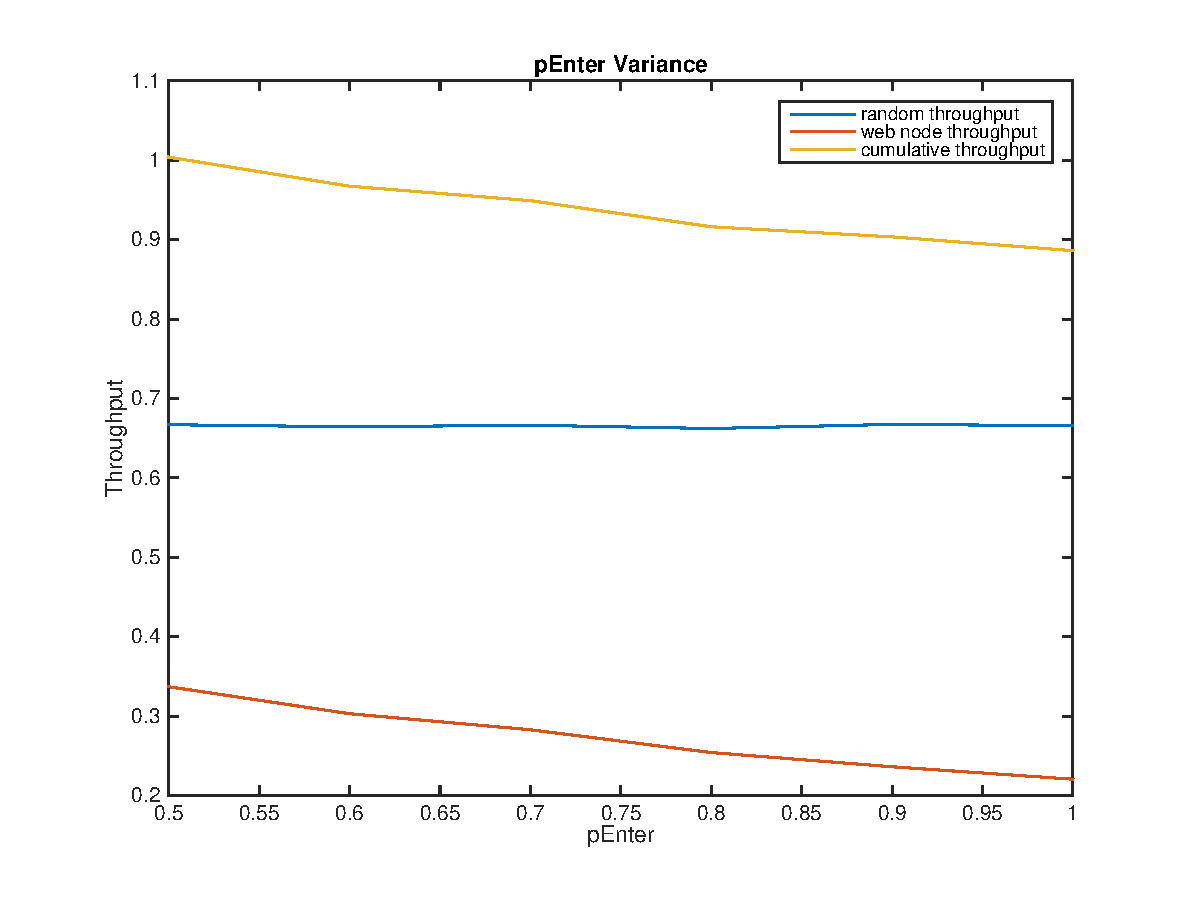
\includegraphics[scale=0.35]{../../src/fig-simulation_random_web-penter-1_0_1_0_1_1_5.eps}

\end{tabular}
\end{figure*}


%%% third
\begin{figure*}
\begin{tabular}{cc}

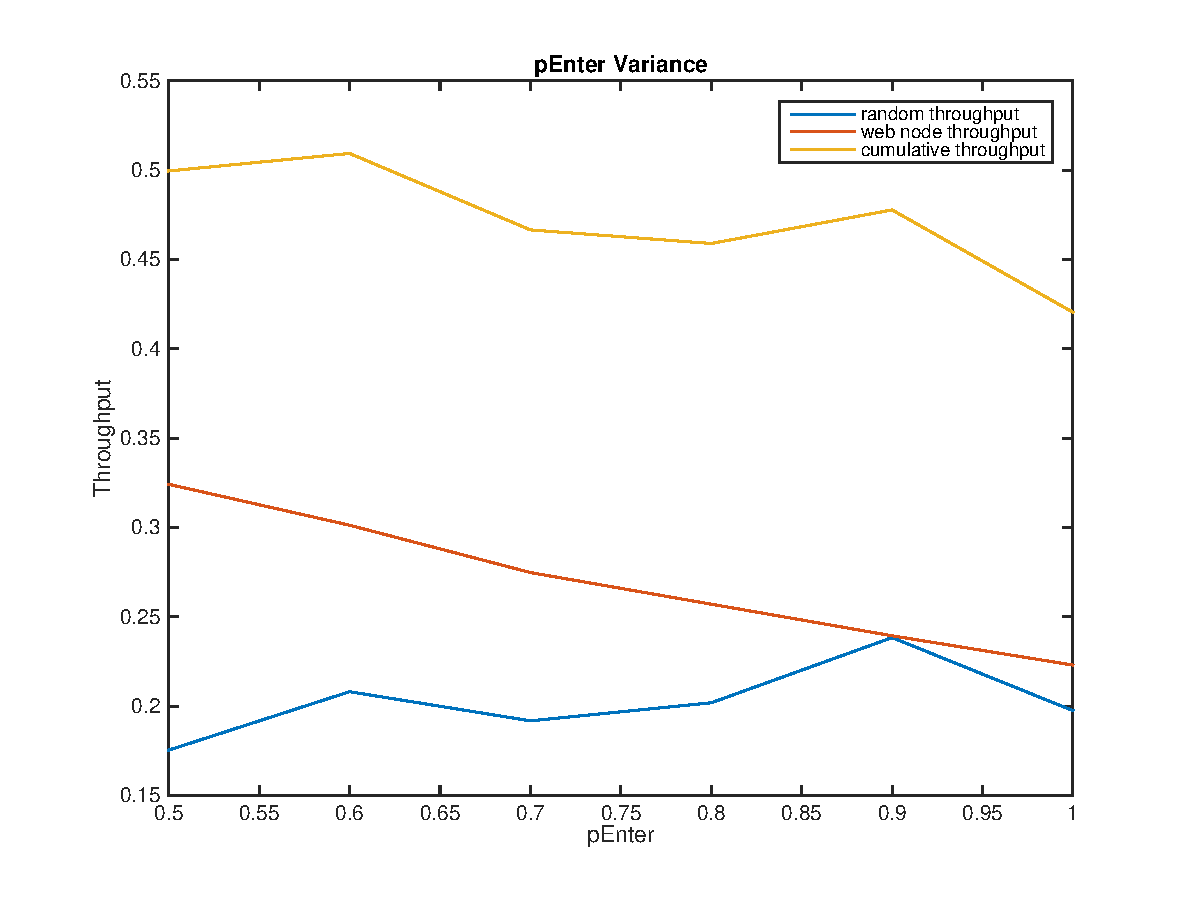
\includegraphics[scale=0.35]{../../src/fig-simulation_random_web-penter-1_0_5_0_1_1_5.eps} & 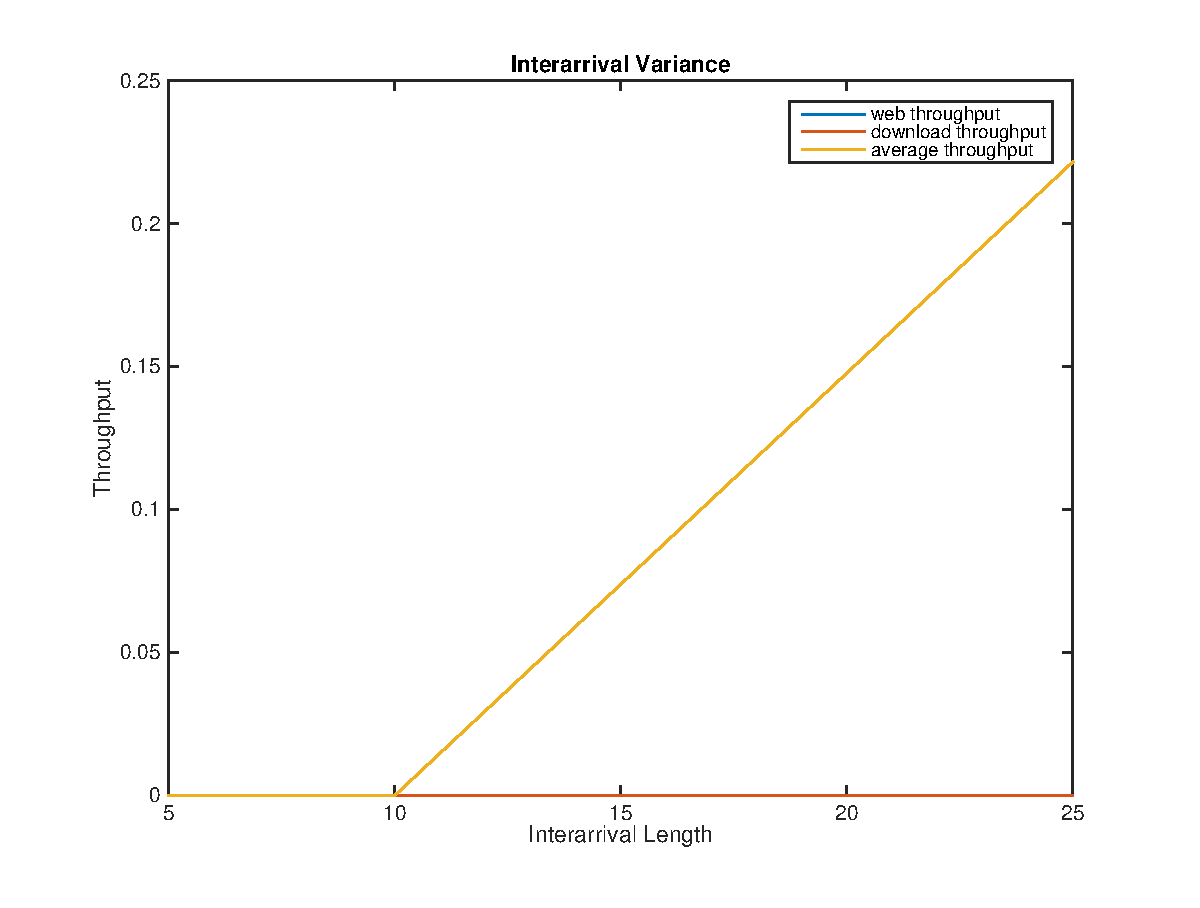
\includegraphics[scale=0.35]{../../src/fig-simulation_web_download-interarival-1_1_1_5_1_1_25.eps} \\
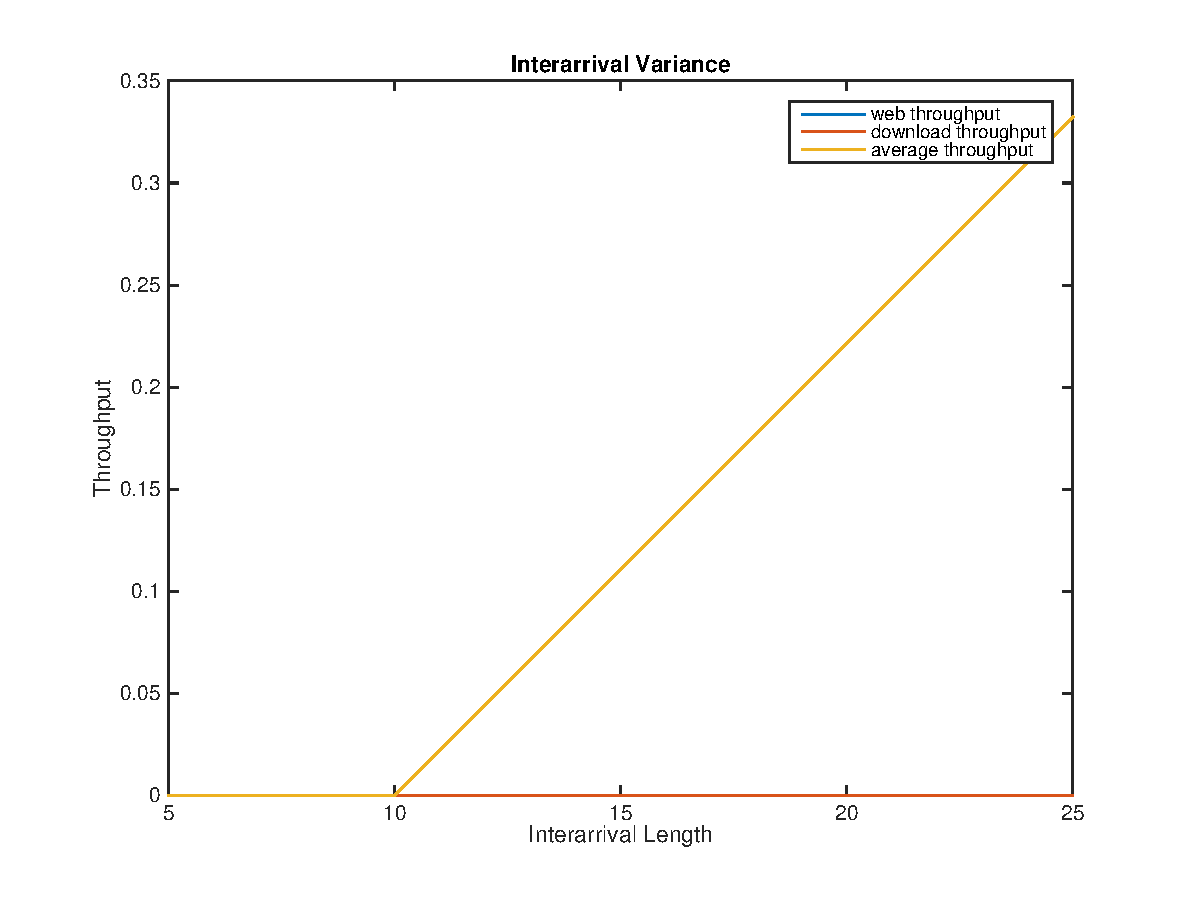
\includegraphics[scale=0.35]{../../src/fig-simulation_web_download-interarival-1_5.000000e-01_1_5_1_1_25.eps} & 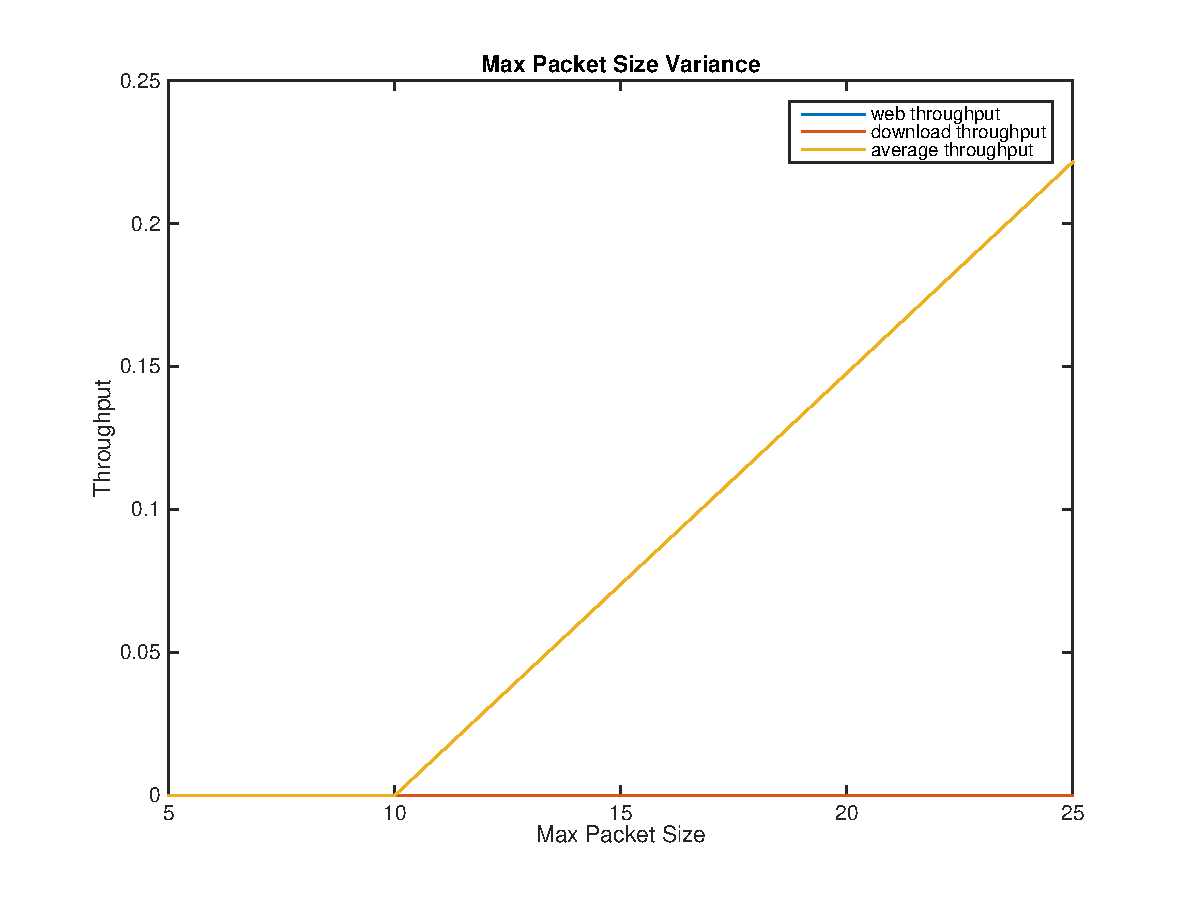
\includegraphics[scale=0.35]{../../src/fig-simulation_web_download-maxpackets-1_1_1_5_1_1_25.eps} \\
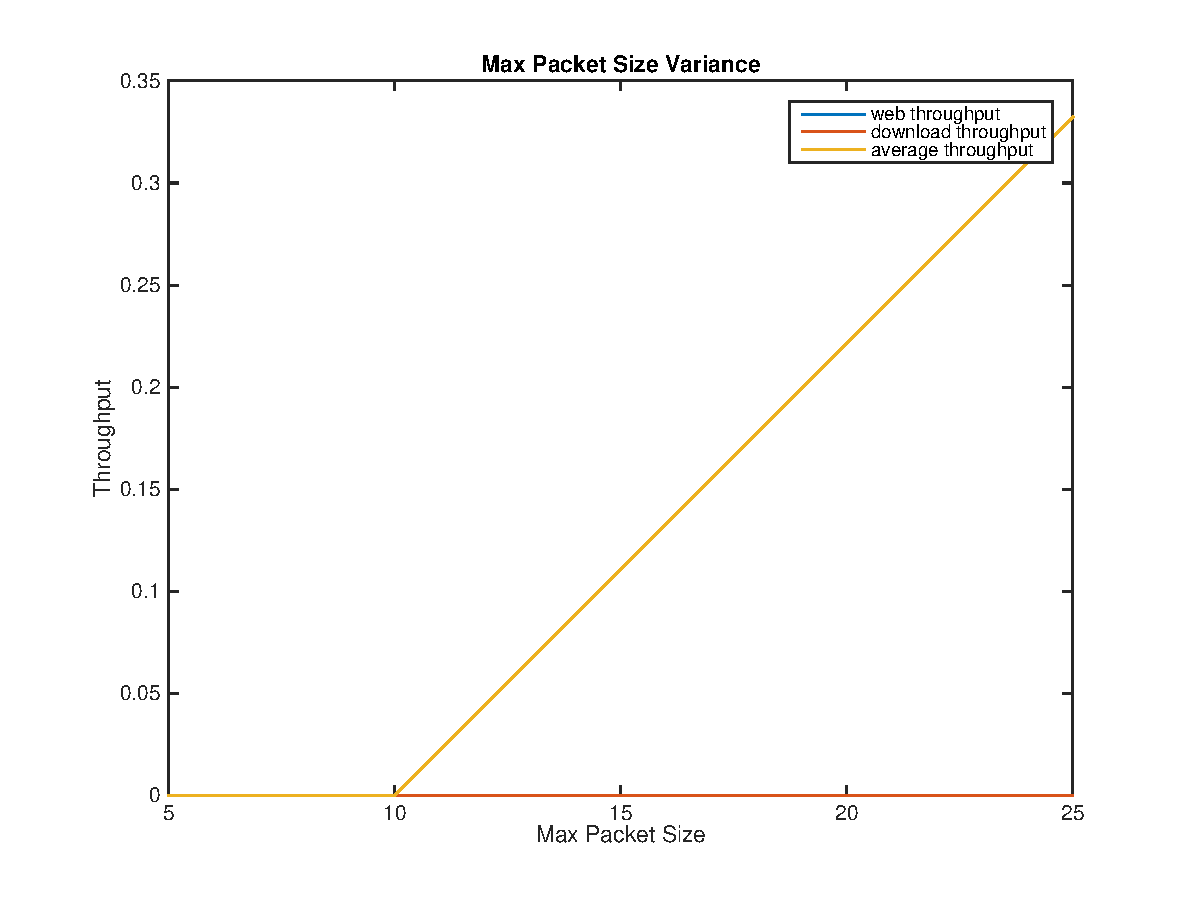
\includegraphics[scale=0.35]{../../src/fig-simulation_web_download-maxpackets-1_5.000000e-01_1_5_1_1_25.eps} & 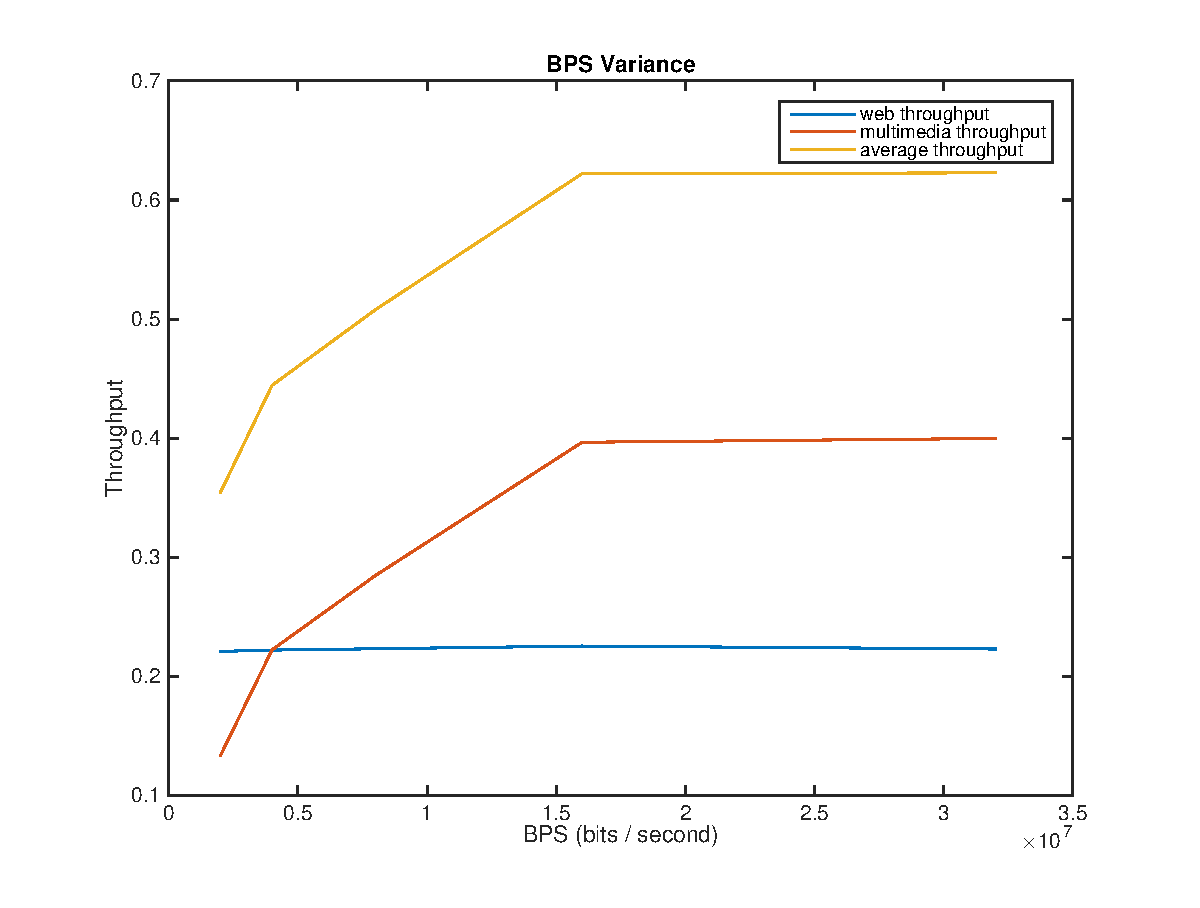
\includegraphics[scale=0.35]{../../src/fig-simulation_web_multimedia-bps-1_1_1_5_12000.eps} \\

\multicolumn{2}{c}{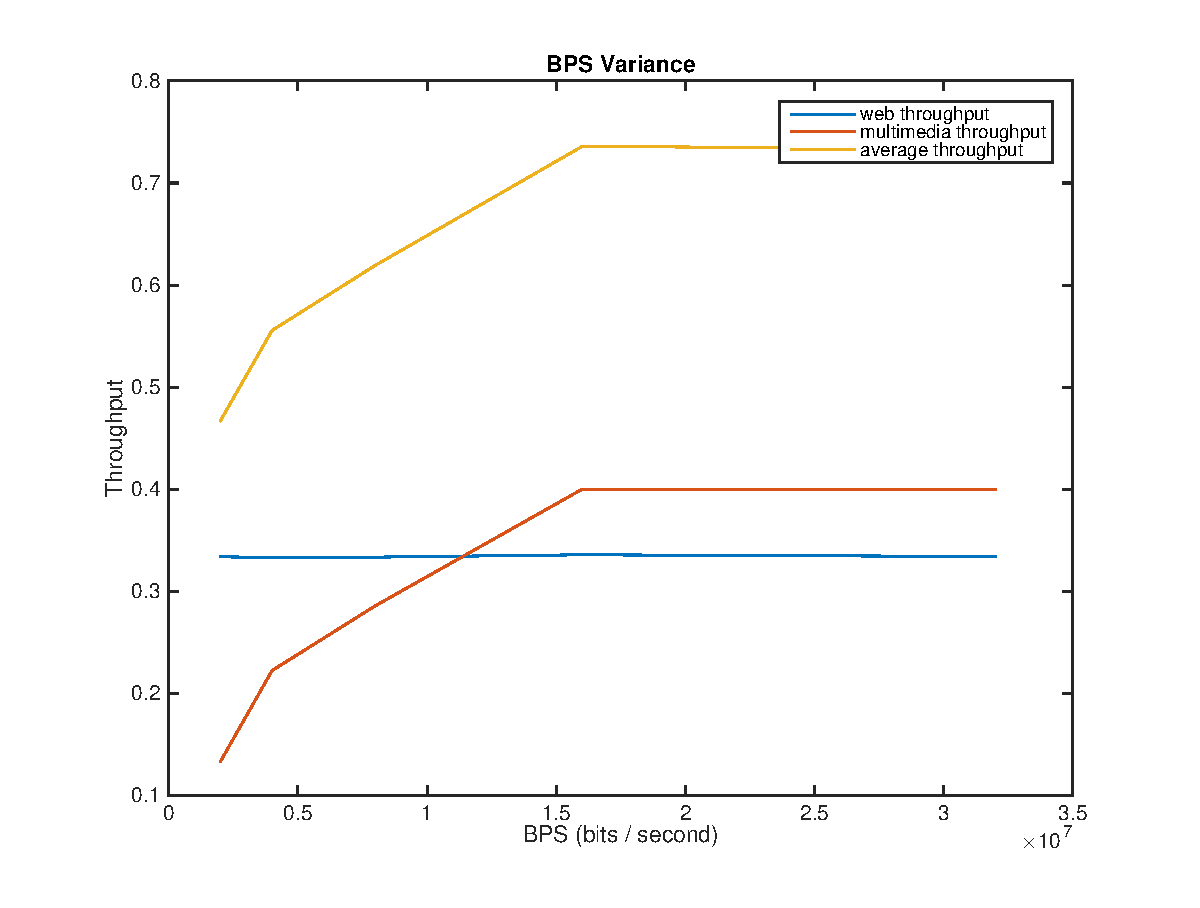
\includegraphics[scale=0.35]{../../src/fig-simulation_web_multimedia-bps-1_5.000000e-01_1_5_12000.eps}}

\end{tabular}
\end{figure*}


\section{Related Work}
Analytical models of the 802.11 DCF function began with Bianchi's seminal work in \cite{bianchi1996performance}. His saturated model was extended to handle non-saturated traffic by Malone et al. in \cite{dcf-nonsaturated} and Zhao et al. in \cite{zhao2009simple} (the latter is a significantly simpler model than the former). In addition to a constant conditional collision probability $p$, the work of Malone et al. includes a per-epoch probability of a packet arrival in the buffer $q$. The authors used this probability to study the performance of non-saturated traffic parameterized by $q$. Nguyen et al. \cite{nguyen2012performance} combine nodes with different saturated and unsaturated characteristics, QoS requirements, and even different backoff timer windows (e.g., $W_{max}$ and $W_{min}$ values). They show that real-time traffic loads are infeasible when the number of nodes exceeds $8$. These results match our observations that multimedia traffic, which can be a type of real-time traffic, starves nodes with more random access patterns.

Qiu et al. \cite{qiu2007general} extended this even further to study the interference caused by an arbitrary number of nodes, and provide additional support for receiver models of packet-loss rates and unicast sender and receiver models. The latter additions are made possible by including model support for senders and receivers of different packets, e.g., data, ACKs, and NACKs. Our work is distinct from this in that we model traffic as a \emph{distributon} of packet types, sizes, lengths, and interarrival times. In addition to this different packet source generation model, the fact that we focus on only two nodes in our simulations (see Section \ref{sec:experiment}) makes it infeasible to compare their results to ours. 

Analysis of the effect of frame buffer sizes was first studied by Zhao et al. in \cite{zhao2011modeling}. However, the goal was not to study the effect of a fixed buffer size used to transport all packets, rather than to study the effect of per-traffic buffer sizes. Li et al. \cite{li2011buffer} also studied the problems and impact of fixed-size buffers in the 802.11 DCF protocol. They found that dynamic buffer sizes, e.g., those tailored to the type of traffic, help achieve high throughput while maintaining low delay across a diverse spread of network and environment conditions. 

In this work, our main goal is to study the performance of the DCF in the presence of hetereogeneous traffic. Others have gone beyond this analysis to propose protocol modifications meant to improve said performance. An example of such work is \cite{li2008predictable}, which presents a variety of algorithms that adapt the DCF for optimal fairness. Another is the work of Gao et al. \cite{gao2013throughput}, in which they study throughput optimization techniques for systems of saturated and unsaturated heterogeneous nodes. However, heterogeneity, in the context of their work, is defined solely with respect to traffic input rates and initial backoff window sizes. Their formal analysis of the individual and system throughput, however, is significantly more involved than our own. In fact, they are able derive sufficient conditions based \emph{only} on the size of saturated groups necessary to achieve the maximal throghput. One such condition is that the initial backoff window of saturated node groups should increase linearly with their size, and that the rate of increase is inversely proportional to the overall group throughput. Again, we do not study the behavior of multinode systems with respect to non-uniform backoff windows, though future work could easily incorporate this extension.

Rozner et al. \cite{rozner2007traffic} study channel assignment techniques based on traffic types found in enterprise WLANs. They frame their analysis in the context of overall system throughput, and conclude that traffic-agnostic access schemes lead to suboptimal throughput measures in random enterprise networks. We do not consider these types of assignment schemes. However, our work is still distinct in that we study the performance using a strictly Markovian model. That is, we do not use simulations built on, for example, NS-3 \cite{henderson2008network}, to study the performance. Our approach lends itself to much more formal and analytical studies. Future work could entail comparing our results against their own.

\section{Conclusion}
In this work we studied the performance of the defacto 802.11 DCF access scheme when serving heterogeneous traffic. We present a novel parameterized Markov model that can used to emulate arbitrary types of application traffic, and then use these models to study the coexistence of said traffic. Our experimental results provide evidence that the deterministic nature of multimedia (e.g., store-and-forward) traffic streams leads to higher performance (i.e., higher throughput) than more nondeteministic (elastic) traffic. Furthermore, our results show that large interarrival time between traffic packets benefits the coexistence of heterogeneous traffic streams. 

\bibliographystyle{IEEEtranS}
\bibliography{ref.bib}

% that's all folks
\end{document}
